\documentclass[12pt]{article}
\usepackage{graphicx} % Required for inserting images
\usepackage{float}
\usepackage{amsmath}
\usepackage{rotating}
\usepackage{verbatim}
\usepackage{listings}
\usepackage{xcolor}
\usepackage{hyperref}



\lstset{
    basicstyle=\ttfamily\footnotesize,
    keywordstyle=\color{blue},
    commentstyle=\color{gray},
    stringstyle=\color{purple},
    numbers=left,
    numberstyle=\tiny,
    stepnumber=1,
    frame=single
}

\begin{document}

\begin{titlepage}
\centering 

\includegraphics[width=2.434cm,height=2.565cm]{./R.png}

\bigskip

{\Large \textbf{UNIVERSIT\`A DEGLI STUDI DI CATANIA}}

{\scshape
\large
Dipartimento di Matematica e Informatica
}

{\scshape
\normalsize
Corso di Laurea Magistrale in Informatica
}

\bigskip


\hrule


\bigskip


\bigskip


\bigskip


\bigskip


{
\large
Denise Cilia \\
Eleonora Giuffrida \\
Valeria Platania 
\par}

\bigskip


\bigskip


\bigskip


\bigskip

{\centering
\Large
\it
PedestriansDET: Sistema di Detection e Conteggio dei pedoni
\par}


\bigskip


\bigskip


\bigskip


\bigskip


\bigskip


\bigskip


\begin{minipage}[b]{8 cm}
\hrule

\bigskip

{\centering\scshape 
Relazione Progetto Machine Learning
\par}



\bigskip

\hrule
\end{minipage}
\bigskip


\bigskip


\bigskip


\bigskip


\bigskip


\bigskip


\bigskip



\bigskip


\bigskip


\bigskip

{\raggedleft
\it
Prof. Giovanni Maria Farinella \\
Dott. Rosario Leonardi 
\par}


\bigskip


\bigskip


\bigskip


\bigskip

\hrule

\bigskip

{\centering
Anno Accademico 2024 - 2025
\par}
\end{titlepage}


\renewcommand{\contentsname}{Indice}
\tableofcontents  % Qui viene inserito l'indice
\newpage
\section{Introduzione}
Nel panorama in continua evoluzione dell'intelligenza artificiale, il Machine Learning si afferma come una disciplina fondamentale, con applicazioni che trovano spazio in numerosi settori. Tra questi, la Computer Vision riveste un ruolo di primaria importanza, e al suo interno, l'Object Detection si distingue come una delle sfide più rilevanti e complesse. \\
Il presente lavoro propone di esplorare e documentare le fasi di sviluppo di un sistema incentrato sul riconoscimento e la localizzazione di esseri umani all'interno di sequenze video e fotogrammi. Il task verrà affrontato sfruttando la comprovata efficacia degli algoritmi della famiglia YOLO (You Only Look Once). Questi modelli si sono affermati per la loro notevole capacità nell'eseguire la rilevazione degli oggetti in tempo reale, caratteristica cruciale per applicazioni che richiedono risposte immediate. \\
In particolare, verranno impiegati e valutati alcuni dei modelli più recenti della serie YOLO, tra cui YOLOv8m, YOLOv10n e YOLOv11s, al fine di identificare la soluzione più idonea in termini di \textit{trade-off} tra accuratezza e performance computazionali per il task specifico. Ai precedenti menzionati seguirà l'uso di Faster RCNN con backbone ResNet50. Le sezioni successive della relazione illustreranno in dettaglio le metodologie adottate, la preparazione del dataset, le fasi di addestramento e le metriche di valutazione impiegate per analizzare le prestazioni dei modelli su un dataset acquisito manualmente. 

\begin{figure}[H]
    \centering
    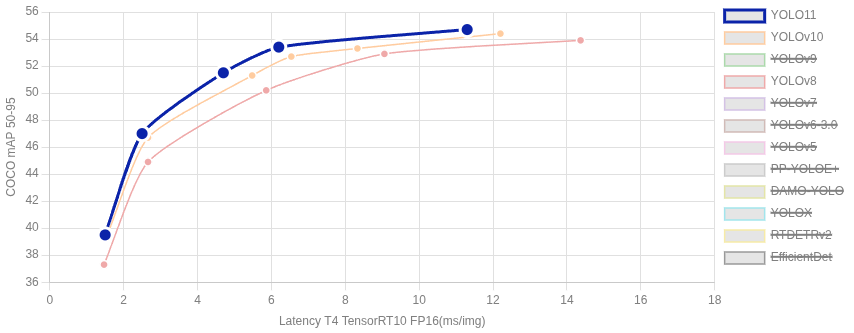
\includegraphics[width=1.1\textwidth]{./img/yolo-model-comparison.png}
    \caption{Confronto delle misure di performance dei modelli YOLO}
    \label{fig:yolo-model-comparison}
\end{figure}

\section{Problema: Object Detection}
\subsection{Descrizione}
L'Object Detection identifica con precisione la posizione di ogni singolo oggetto di interesse presente in un'immagine e lo classifica assegnando una classe di appartenenza. Si prenda come esempio pratico il voler individuare tutte le persone presenti in un filmato: l'Object Detection non solo dirà che sono presenti delle persone, ma disegnerà un riquadro, la cosiddetta \textit{bounding box}, attorno a ciascuna di esse, fornendo le loro coordinate esatte.
Dunque, un algoritmo di Object Detection può essere visto come l'unione di due componenti fondamentali:
\begin{itemize}
    \item Un algoritmo di classificazione: il suo compito è determinare a quale categoria appartiene l'oggetto individuato. Nel nostro caso, si tratterà di stabilire se un determinato elemento è un essere umano.
    \item Un algoritmo di regressione: questo componente si occupa di definire con esattezza la posizione e le dimensioni della \textit{bounding box}, ovvero il riquadro che racchiude l'oggetto. È grazie a questa parte che possiamo localizzare precisamente ogni individuo all'interno di un frame.
\end{itemize}


\subsection{Applicazioni pratiche}
L'importanza di questa task si evince in una moltitudine di contesti pratici. Si prenda d'esempio la sicurezza e la sorveglianza, dove sistemi intelligenti possono monitorare aree, rilevare presenze non autorizzate o analizzare comportamenti sospetti, come nel caso di presenza di intrusi in aree riservate o con accesso vietato. Oppure ancora, nel settore della robotica e automazione nel quale i robot possono essere dotati di un sistema visivo per interagire con l'ambiente circostante, riconoscendo ostacoli o la presenza e la posizione di operatori umani per garantire la sicurezza e facilitare la collaborazione. Anche nel campo dell'analisi del comportamento umano, l'Object Detection di persone in video permette di studiare le interazioni sociali. \\
Lo studio, focalizzato sul riconoscimento di esseri umani in sequenze video e fotogrammi, si inserisce pienamente nel contesto di \textit{pedestrian detection} che trova estensione anche nel campo dell'\textbf{ADAS} (Advanced driver-assistance system) per il supporto ai sistemi di sicurezza delle macchine con guida autonoma.

\begin{figure}[H]
    \centering
    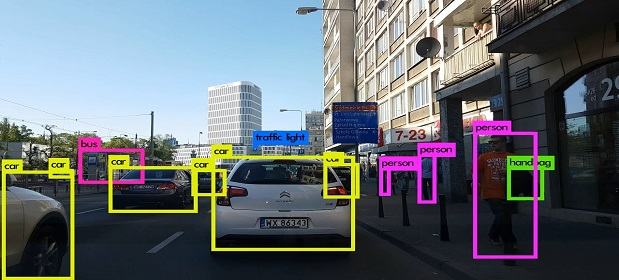
\includegraphics[width=0.80\textwidth]{./img/object-detection-example0.jpg}
    \caption{Object Detection applicata alla guida autonoma}
    \label{fig:adas-example}
\end{figure}

\begin{figure}[H]
    \centering
    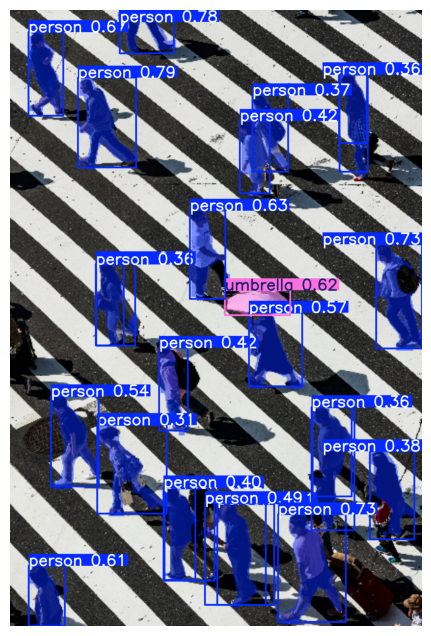
\includegraphics[width=0.50\textwidth]{./img/object-detection-example2.png}
    \caption{Object Detection applicata al riconoscimento di pedoni}
    \label{fig:pedestrians-example}
\end{figure}

\section{Reti Neurali Convoluzionali (CNN)}
E' essenziale comprendere le fondamenta su cui poggiano gran parte degli algoritmi di Computer Vision moderni: le Reti Neurali Convoluzionali (CNN). Le CNN agiscono come degli "occhi" artificiali estremamente sofisticati, capaci di imparare a riconoscere pattern e caratteristiche visive direttamente dai dati. A differenza delle reti neurali tradizionali, le CNN sono state progettate specificamente per elaborare dati strutturati come le immagini, sfruttando strati convoluzionali che applicano filtri per estrarre caratteristiche gerarchiche, dai bordi a texture più semplici fino a forme e oggetti complessi.\\ 
Mentre YOLO ha rivoluzionato il campo con il suo approccio \textit{single-stage}, è importante riconoscere che esistono anche architetture \textit{two-stage} che hanno contribuito enormemente allo sviluppo dell'Object Detection, offrendo spesso un'accuratezza superiore, seppur a discapito dei tempi di elaborazione. Tra queste, Faster R-CNN si è affermata come una pietra miliare, rappresentando un'evoluzione significativa rispetto ai suoi predecessori (R-CNN e Fast R-CNN). Segue la trattazione nel dettaglio di entrambi gli approcci.

\subsection{YOLO - "You Only Look Once"}
Nel campo dell'Object Detection, l'introduzione di YOLO\cite{YOLO} (You Only Look Once) ha segnato una vera e propria svolta, ridefinendo gli standard di velocità ed efficienza. A differenza degli approcci precedenti, che spesso prevedevano più passaggi per identificare e classificare gli oggetti, YOLO ha introdotto il paradigma \textit{single-stage}. Questo significa che il modello è in grado di predire contemporaneamente sia le posizioni degli oggetti (precisamente le bounding box) sia le loro classi di appartenenza, il tutto in un unico passo. Questa caratteristica intrinseca ha permesso a YOLO di eccellere nella detection. \\
Dalla sua prima apparizione nel 2015, la filosofia di YOLO ha dato vita a una serie di evoluzioni, ognuna delle quali ha introdotto miglioramenti significativi in termini di accuratezza, velocità e robustezza. Nello studio vengono confrontate alcune delle versioni più recenti e performanti di questa famiglia, ognuna con le sue peculiarità e ottimizzazioni.

\begin{figure}[H]
    \centering
    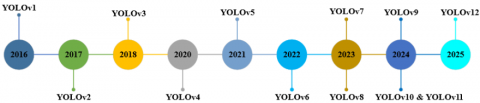
\includegraphics[width=1.0\textwidth]{./img/yolo-timeline.png}
    \caption{Release timeline dei modelli YOLO}
    \label{fig:yolo-timeline}
\end{figure}


\begin{figure}[H]
    \centering
    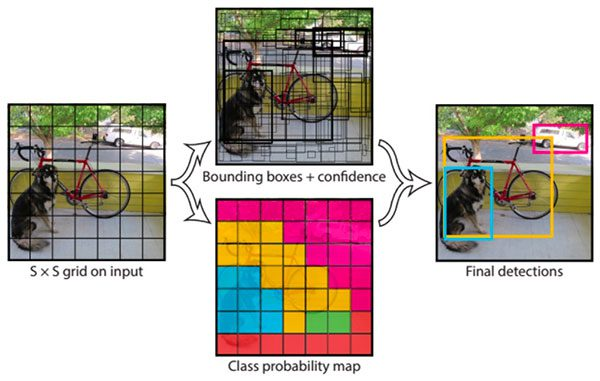
\includegraphics[width=1.1\textwidth]{./img/yolo-single-stage.jpg}
    \caption{Funzionamento single-stage in YOLO}
    \label{fig:yolo-single-stage}
\end{figure}

\subsubsection{YOLOv8 Medium} 
Basandosi sulla filosofia "You Only Look Once" (YOLO), che processa l'intera immagine in un'unica passata per predire contemporaneamente posizioni dei \textit{bounding box} e classi di appartenenza, il modello porta avanti questa tradizione con significative innovazioni.\\
Questa implementazione si distingue per una serie di miglioramenti architetturali e funzionali che ne aumentano l'efficienza e l'accuratezza. Presenta un'architettura \textit{Anchor-Free}: anziché la tradizionale detection basata sulle anchor, YOLOv8 utilizza un approccio che permette di rendere la fase di \textit{training} ancora più semplice e aiuta il modello a lavorare bene su dataset diversi. È stato progettato per essere un modello versatile, capace di gestire non solo l'Object Detection, ma anche compiti correlati come l'\textit{Image Segmentation} e la \textit{Pose Estimation}, rendendolo una soluzione più completa per diverse applicazioni di Computer Vision. L'approccio di questa versione si concentra sull'offrire un framework robusto e facile da usare, che permette agli sviluppatori di implementare rapidamente soluzioni di rilevamento oggetti ad alte prestazioni.

\subsubsection{YOLOv10 Nano} Con l'arrivo di YOLOv10, i ricercatori della Tsinghua University hanno introdotto un approccio innovativo, mirato a superare alcune delle limitazioni delle versioni precedenti, in particolare nella post-elaborazione e nell'architettura del modello. La versione \textit{nano} (YOLOv10n) è stata progettata per offrire prestazioni elevate anche in ambienti con risorse computazionali limitate, pur mantenendo un'ottima accuratezza. Un aspetto distintivo di YOLOv10 è l'eliminazione del meccanismo di Non-Maximum Suppression (\textbf{NMS}) durante la fase di training, un processo tradizionalmente utilizzato per rimuovere le predizioni ridondanti. Questa innovazione è resa possibile dalla strategia chiamata Dual Label Assignment with NMS-free training. In sintesi, YOLOv10 combina un approccio \textit{one-to-one matching}, ovvero assegna una singola predizione a ogni oggetto, eliminando la necessità di NMS con la più tradizionale \textit{one-to-many assignment}. Quest'ultima garantisce performance migliori ma richiede NMS. L'introduzione di un \textit{one-to-one head} aggiuntivo, ottimizzato congiuntamente al \textit{one-to-many head} tramite una \textit{Consistent Matching Metric}, permette di ottenere i benefici di entrambi gli approcci, migliorando l'accuratezza e la convergenza.
    
\subsubsection{YOLOv11 Small} 
Il modello si concentra sull'affinare l'equilibrio tra velocità e accuratezza, un aspetto cruciale per le applicazioni pratiche. Tra le sue innovazioni, spicca l'aumento di accuratezza rispetto ai modelli precedenti. YOLOv11\cite{YOLOv11} utilizza \textit{loss functions} più complesse, migliorando le \textit{anchor boxes} e evidenziando la tecnica di \textit{data augmentation}. Con quest'ultime, il modello riesce ad individuare gli oggetti anche in contesti non semplici. YOLOv11 migliora anche l'uso delle risorse hardware, riducendo sensibilmente i tempi di training e costi computazionali.



\subsection{Faster R-CNN: Two-Stage Approach}
L'approccio \textit{two-stage} nell'Object Detection si distingue per la sua metodologia di rilevamento degli oggetti, suddivisa in due fasi principali e sequenziali. Nella prima fase, il sistema si concentra sull'identificazione delle aree dell'immagine che più probabilmente contengono un oggetto, generando un insieme di "proposte di regione". La seconda fase prende queste proposte e le analizza in dettaglio, classificando l'oggetto all'interno di ciascuna regione e affinando la posizione del suo bounding box. Questo processo in due passaggi, pur introducendo una maggiore complessità computazionale rispetto ai metodi \textit{single-stage}, consente di raggiungere un'accuratezza superiore, rendendo questi modelli ideali per applicazioni dove la precisione è la priorità assoluta.\\
Questo approccio affonda le sue radici nella ricerca sull'Object Detection, nascendo dalla necessità di superare le inefficienze dei metodi precedenti. Inizialmente, i sistemi si affidavano a tecniche di \textit{sliding window}, che scansionavano l'intera immagine con finestre di diverse dimensioni e proporzioni per classificare il contenuto di ogni porzione. Questo processo, tuttavia, si rivelava computazionalmente proibitivo e inefficiente.\\
La svolta si è avuta con l'introduzione delle architetture basate su Region-based Convolutional Neural Networks (R-CNN). L'idea innovativa consisteva nel generare un numero limitato di proposte di regione e concentrare la classificazione e la regressione dei bounding box solo su queste. Questo ha ridotto drasticamente il carico computazionale. Le successive evoluzioni, come Fast R-CNN, hanno ulteriormente ottimizzato questo processo, ma persistevano ancora colli di bottiglia legati alla generazione separata delle proposte e alla loro elaborazione.\\
È in questo contesto di continua ricerca di efficienza e precisione che Faster R-CNN\cite{FasterRCNN} si è affermata come una pietra miliare. Questa architettura ha perfezionato l'approccio \textit{two-stage} integrando la generazione delle proposte di regione direttamente all'interno della rete neurale, attraverso il Region Proposal Network (RPN). Ciò ha reso l'intero processo \textit{end-to-end} e significativamente più efficiente. Il funzionamento dettagliato di questo approccio, in particolare di Faster R-CNN, verrà approfondito nel Capitolo 5. 
\begin{figure}[H]
    \centering
    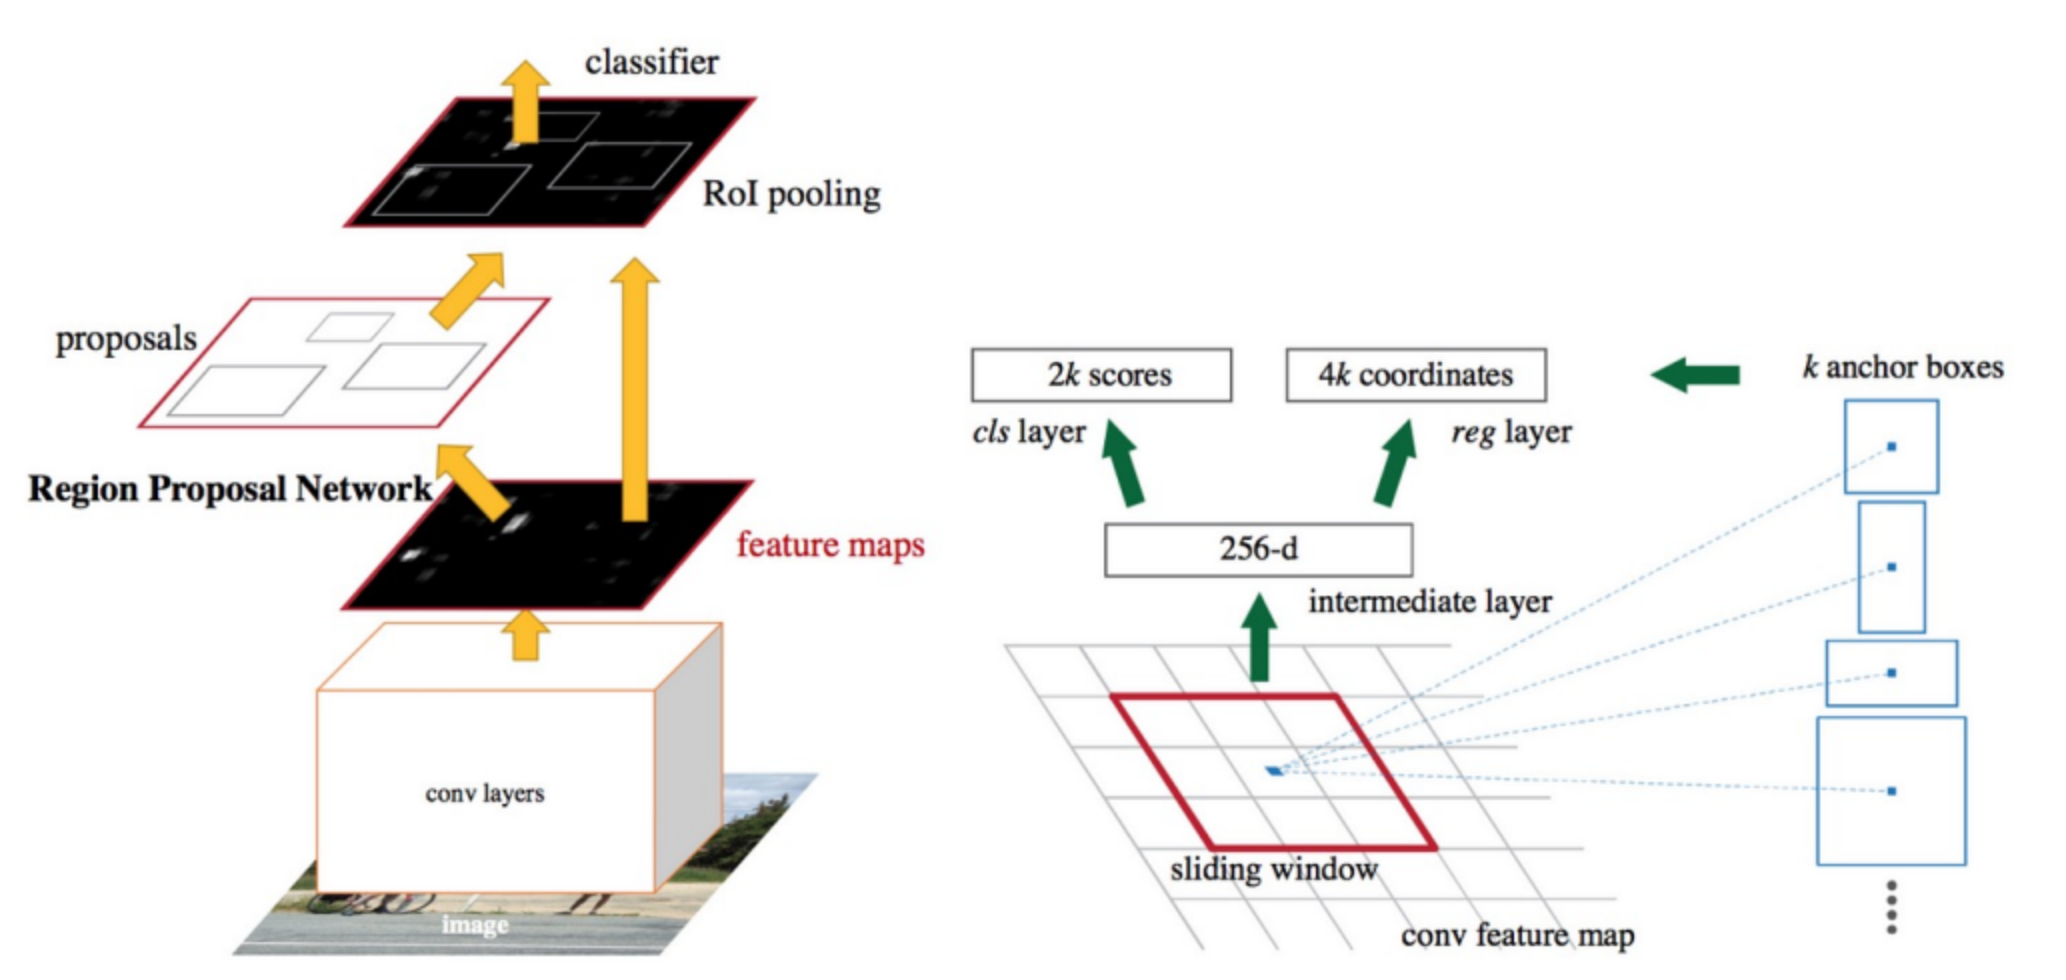
\includegraphics[width=1.1\textwidth]{./img/faster-rcnn-two-stage.png}
    \caption{Architettura Faster RCNN}
    \label{fig:faster-rcnn}
\end{figure}
\subsubsection{ResNet50}
ResNet50\cite{ResNet50} è una rete neurale convoluzionale profonda composta da 50 strati, appartenente alla famiglia delle \textit{Residual Networks}, introdotte da He et al. nel 2015. La sua architettura è progettata per affrontare il problema della degradazione delle prestazioni nelle reti molto profonde, grazie all’introduzione delle \textbf{connessioni residue} (\textit{skip connections}). Queste connessioni permettono di far fluire l’informazione direttamente da uno strato all’altro, saltando uno o più layer intermedi, favorendo così un addestramento più stabile e una convergenza più rapida.\\
La struttura di ResNet50 si basa su una sequenza iniziale di convoluzione 7$\times$7 con 64 filtri e \textit{stride} pari a 2, seguita da un livello di \textit{Max Pooling} 3$\times$3. L’architettura è quindi suddivisa in quattro blocchi principali, ciascuno composto da più unità residuali. Ogni unità è implementata tramite uno schema a \textbf{bottleneck}, con tre convoluzioni in sequenza: una 1$\times$1 per la riduzione della dimensionalità, una 3$\times$3 per l’estrazione delle caratteristiche spaziali, e una 1$\times$1 per l’espansione dei canali. Questo design consente di mantenere un buon compromesso tra efficienza computazionale e capacità espressiva.\\
I blocchi successivi aumentano progressivamente il numero di canali: 256, 512, 1024 e 2048, mentre la risoluzione spaziale viene ridotta tramite \textit{stride} pari a 2 nelle prime convoluzioni di ciascun blocco (eccetto il primo). Tutte le unità bottleneck sono collegate alle loro rispettive \textit{skip connections}, implementate tramite addizione element-wise, che permettono un flusso diretto del gradiente anche nei livelli più profondi.\\
Per via della sua architettura bilanciata, ResNet50 rappresenta una scelta solida come \textbf{backbone} nei modelli di \textit{object detection} come Faster R-CNN, in quanto fornisce feature map ricche e gerarchiche senza un costo computazionale eccessivo. In questo progetto, è stata adottata per la sua comprovata efficacia nel riconoscimento visivo e per la sua ampia disponibilità nei principali framework di deep learning.
%immagine resnet50

\begin{figure}[H]
    \centering
    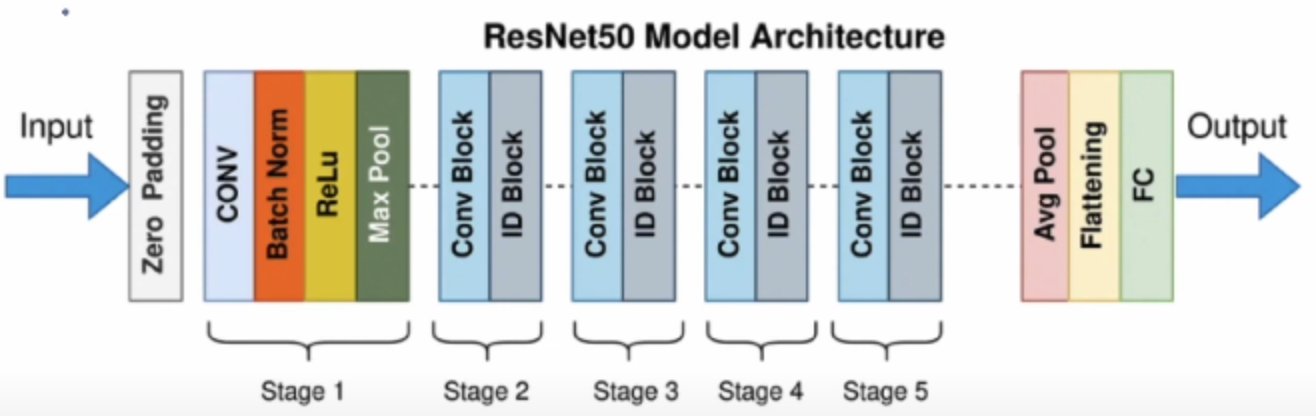
\includegraphics[width=1.00\textwidth]{./img/resnet50.png}
    \caption{Architettura ResNet50}
    \label{fig:resnet50}
\end{figure}


\section{Dataset}
Per la corretta esecuzione dello studio sono stati previsti \textbf{due diversi} dataset elaborati manualmente per adattarli meglio al progetto. In ordine:
\begin{itemize}
    \item Il primo dataset, chiamato \textbf{New Dataset For Machine Learning Project}, è stato utilizzato per la fase di \textbf{training} dei diversi modelli.
    \item Il secondo dataset è stato acquisito personalmente, ed è stato utilizzato per la fase di \textbf{testing} dei modelli presentati nello studio.
\end{itemize}
\subsection{ND4ML (New Dataset For Machine Learning Project)}
Il dataset usato per la fase di training dei modelli è il dataset \textbf{New Dataset For Machine Learning Project} \cite{Roboflow}. Questo dataset è la combinazione di quattro dataset che contengono frame estratti da brevi video, incentrati sul rilevamento di pedoni, e persone più in generale. Si tratta di dataset accessibili pubblicamente sulla piattaforma \textbf{Roboflow}, che mette a disposizione diversi tools per poter annotare frame attraverso interfaccia grafica, e non solo. I dataset, in ordine, possono essere trovati con i seguenti nomi: \textbf{MOT17-03-DPM}, \textbf{Human Detection}, \textbf{People Detection} ed infine \textbf{GTA\_dataset}. L'ultimo dataset è stato personalmente acquisito mediante registrazione schermo sul videogioco \textbf{GTA V} e successivamente annotato manualmente mediante Roboflow. Si tratta di un dataset sintetico che prende fortemente ispirazione dall'articolo \textbf{MOTSynth}\cite{MOTSynth}; l'idea è quella di aumentare ulteriormente le dimensioni del dataset finale in modo da evitare l'overfitting dei modelli, fornendo anche un'ampia diversificazione nei frame che verranno utilizzati per l'allenamento. Difatti, i frame presenti nel dataset finale sono tutti in diverse condizioni di illuminazione, posa, e orientamento. \\
Nel dataset sono presenti un totale di \textbf{2985} immagini di cui \textbf{2015} immagini vengono utilizzate per il training, \textbf{531} per la fase di validation e \textbf{439} per la fase di testing. Tuttavia, sebbene sia presente lo split per il test la fase di testing verrà comunque effettuata su un altro dataset personalmente acquisito. Tutte le immagini sono state salvate in formato \texttt{.jpg} e hanno una dimensione variabile, generalmente \textbf{1920x1080}. Inoltre sono presenti diverse classi: 0, pedestrian, 1, 2, 3, 4, 5, 6, 7. Nella sottosezione pre-processing verrà approfondito come queste classi sono state riformulate per poterle meglio adattare allo studio. In particolare, per ogni annotazione verrà generato un corrispondente file nel formato desiderato (ad esempio YOLO oppure COCO JSON) che indicherà come nel caso di YOLO la bounding box: 
\begin{center}
    $<class><x\_center><y\_center><width><height>$
\end{center}
Di seguito è possibile visualizzare degli esempi di frame del dataset utilizzato.

\begin{figure}[H]
    \centering
    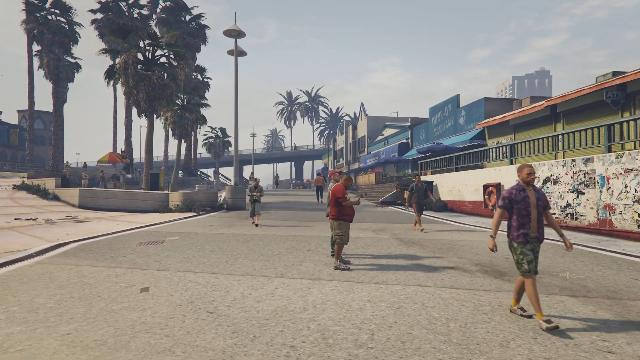
\includegraphics[width=1.00\textwidth]{./img/gta-original.jpg}
    \caption{Frame sintentico del dataset senza ground-truth}
    \label{fig:gta-frame}
\end{figure}

\begin{figure}[H]
    \centering
    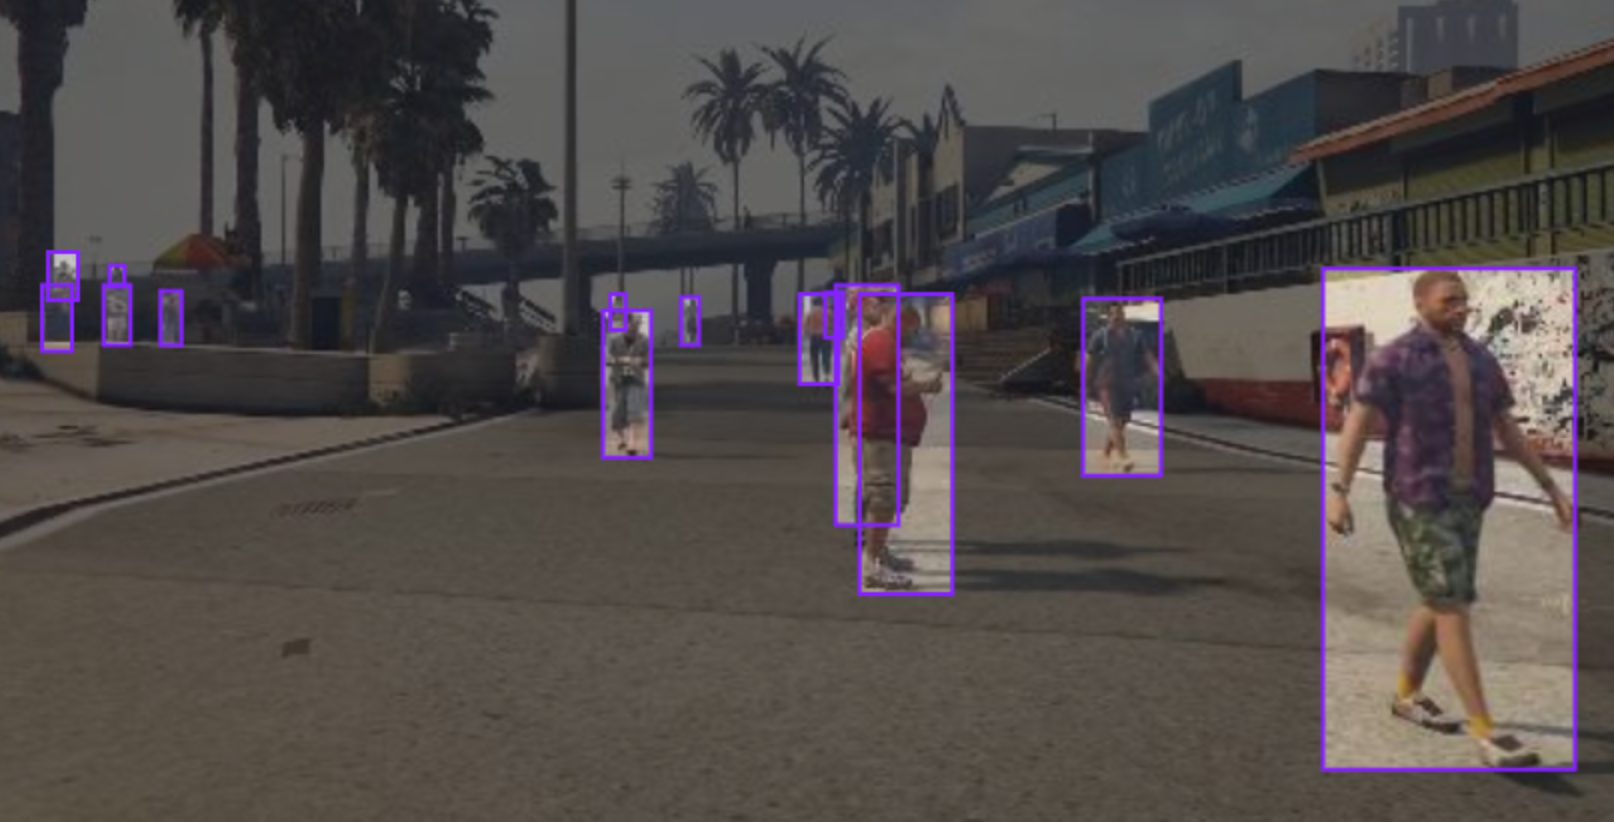
\includegraphics[width=1.00\textwidth]{./img/gta-ground-truth.png}
    \caption{Frame sintentico del dataset con ground-truth}
    \label{fig:gta-frame-2}
\end{figure}

\begin{figure}[H]
    \centering
    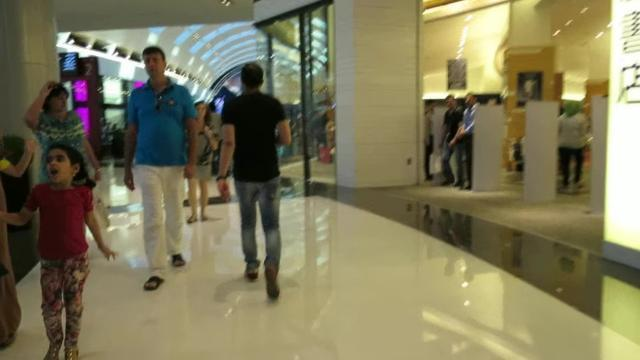
\includegraphics[width=1.00\textwidth]{./img/dataset-original.jpg}
    \caption{Frame del dataset senza ground-truth}
    \label{fig:dataset-frame}
\end{figure}

\begin{figure}[H]
    \centering
    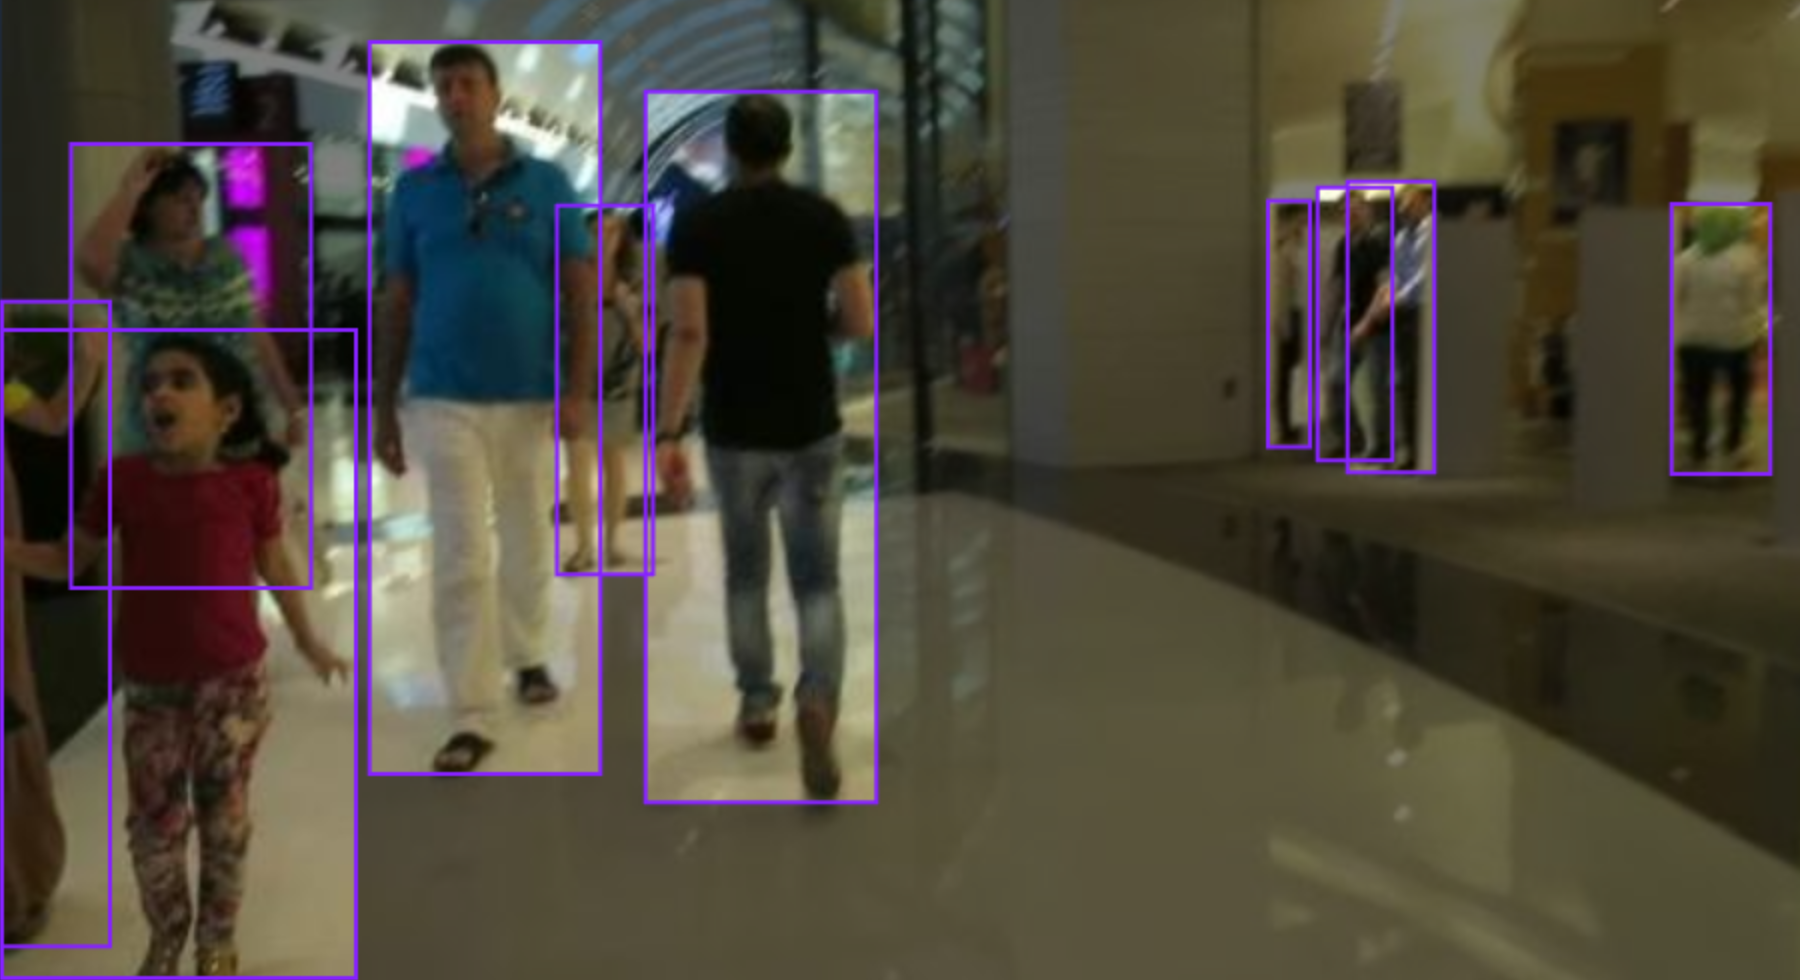
\includegraphics[width=1.00\textwidth]{./img/dataset-ground-truth.png}
    \caption{Frame del dataset con ground-truth}
    \label{fig:dataset-frame-2}
\end{figure}

\begin{figure}[H]
    \centering
    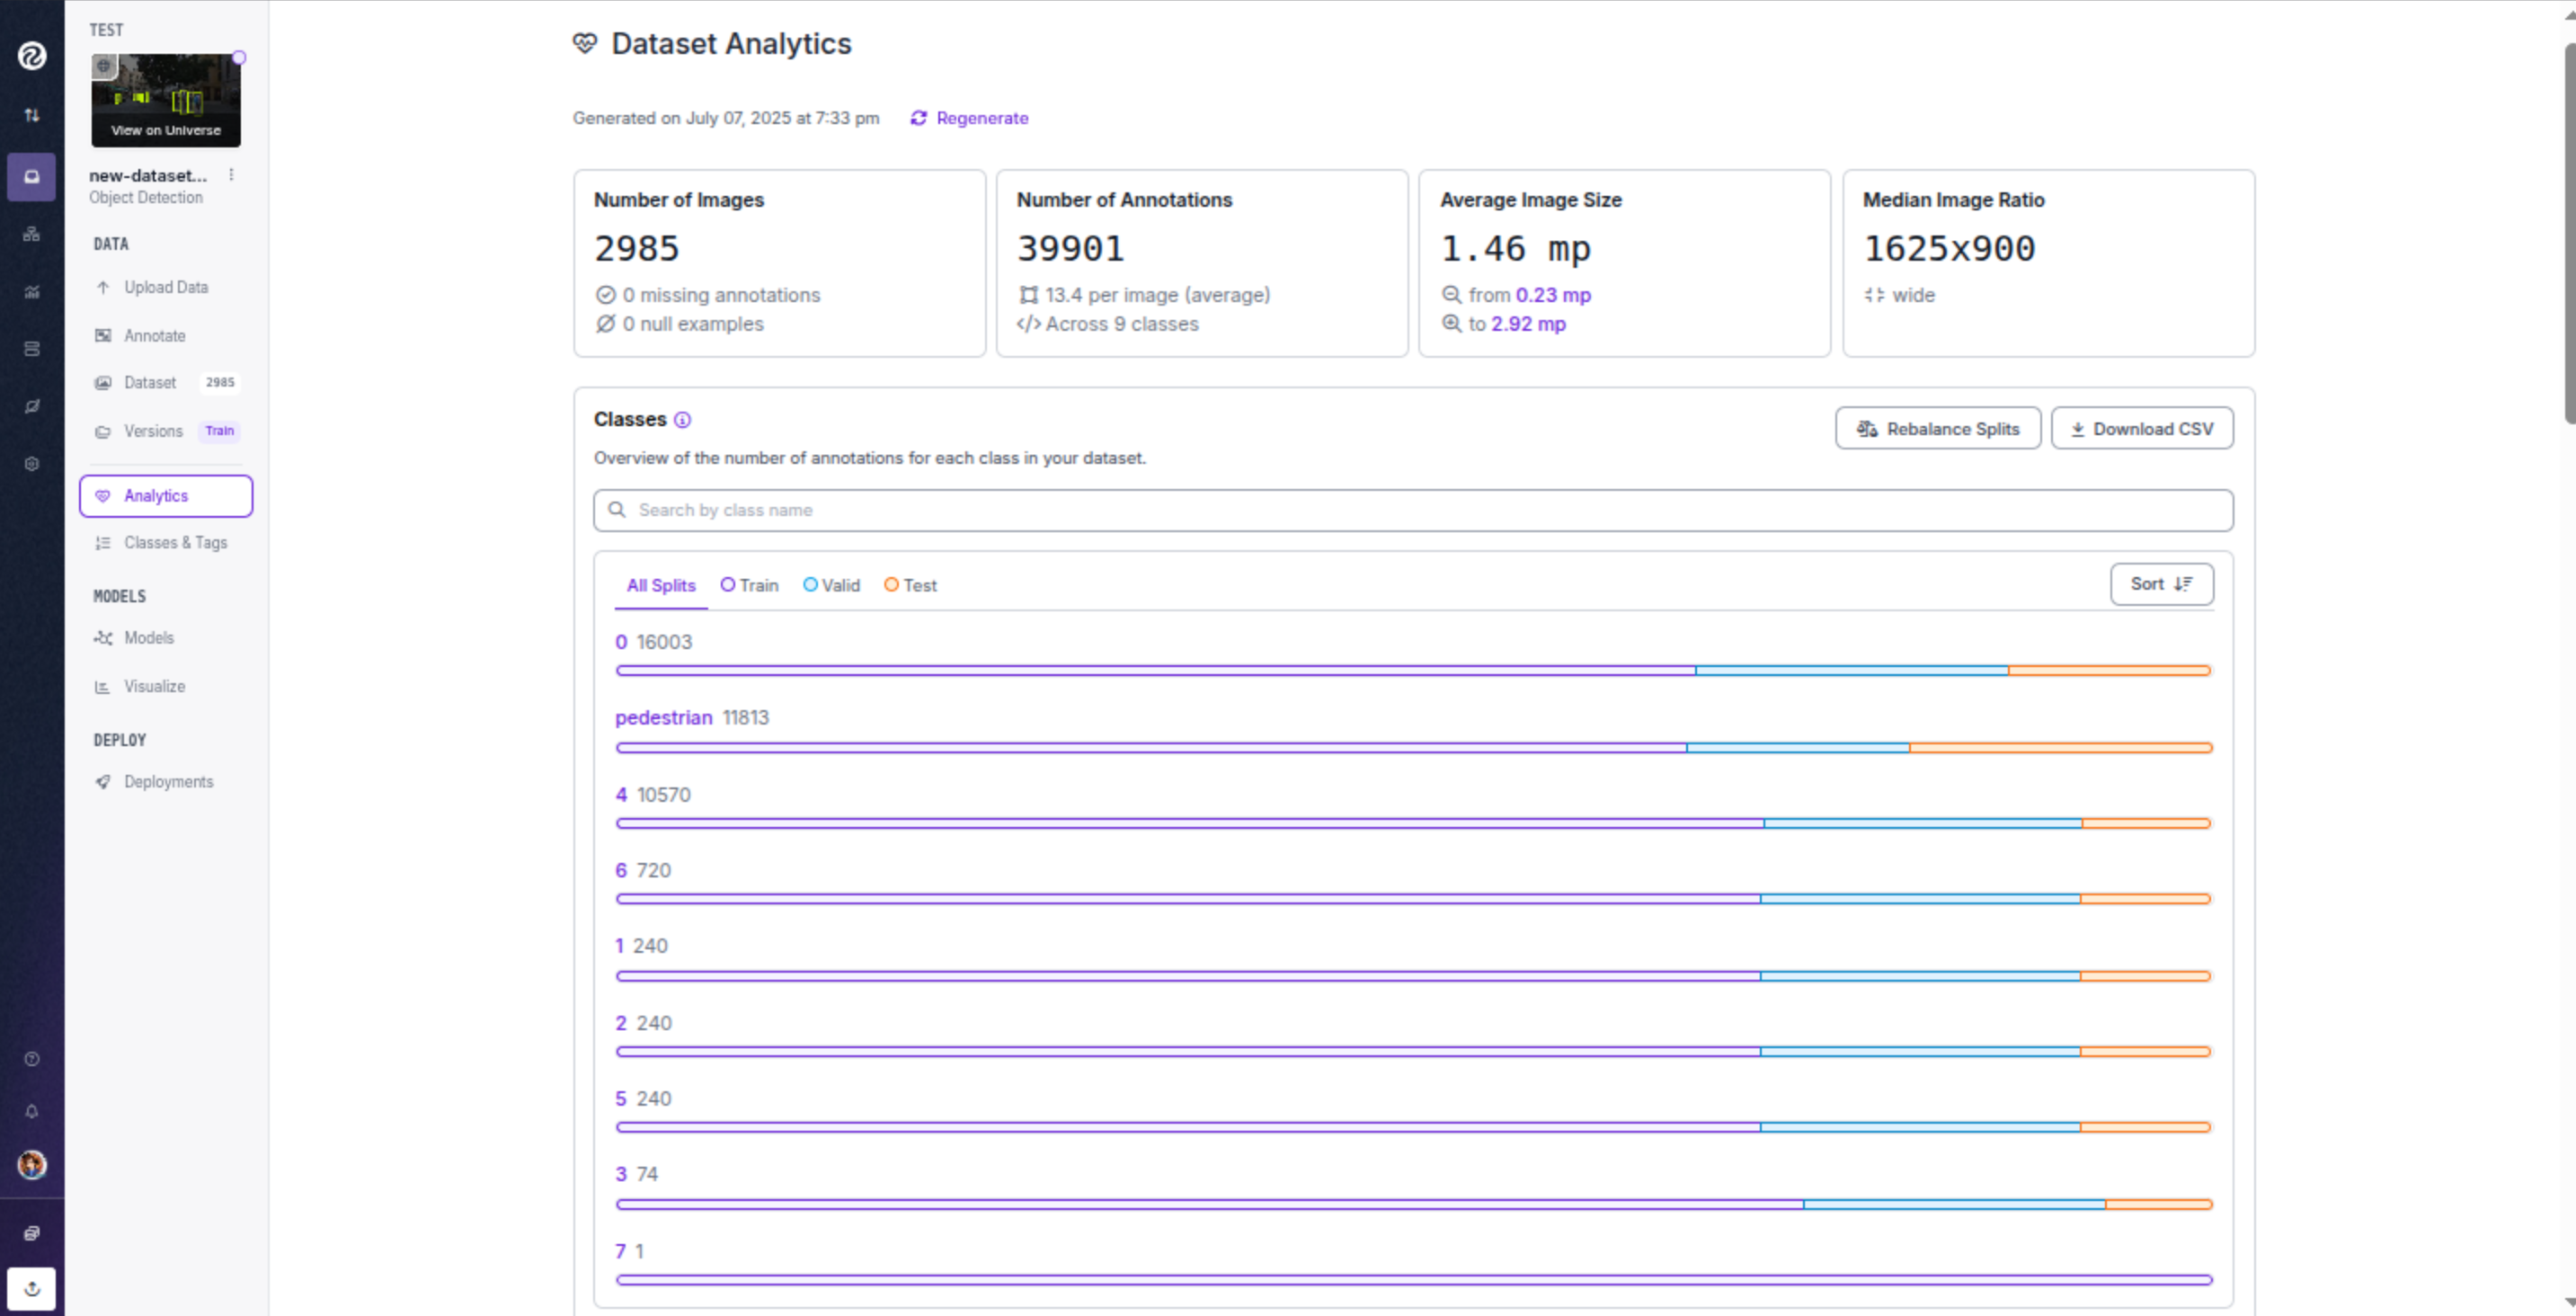
\includegraphics[width=1.0\textwidth]{./img/roboflow-dataset.png}
    \caption{Statistiche sul dataset calcolate su Roboflow}
    \label{fig:roboflow-dataset}
\end{figure}

\subsection{Dataset acquisito per la fase di test}
Allo scopo di effettuare la fase di testing del modello su dati mai visti prima, è stato realizzato un nuovo dataset formato da tre brevi video successivamente frammentati in singole immagini. Il dataset è stato acquisito nel centro di \textbf{Catania}. Contiene al suo interno immagini acquisite attraverso un dispositivo \textbf{iPhone 15} a risoluzione originale \textbf{1920x1080} camminando per le strade del centro catanese. I video sono stati acquisiti con diverse condizioni di illuminazione e cercando di ottenere diverse angolazioni, pur sempre simili alle angolazioni presenti invece nel dataset usato per il training. \\
I frame ottenuti dai video sono stati annotati attraverso \textbf{Roboflow}.

\begin{figure}[H]
    \centering
    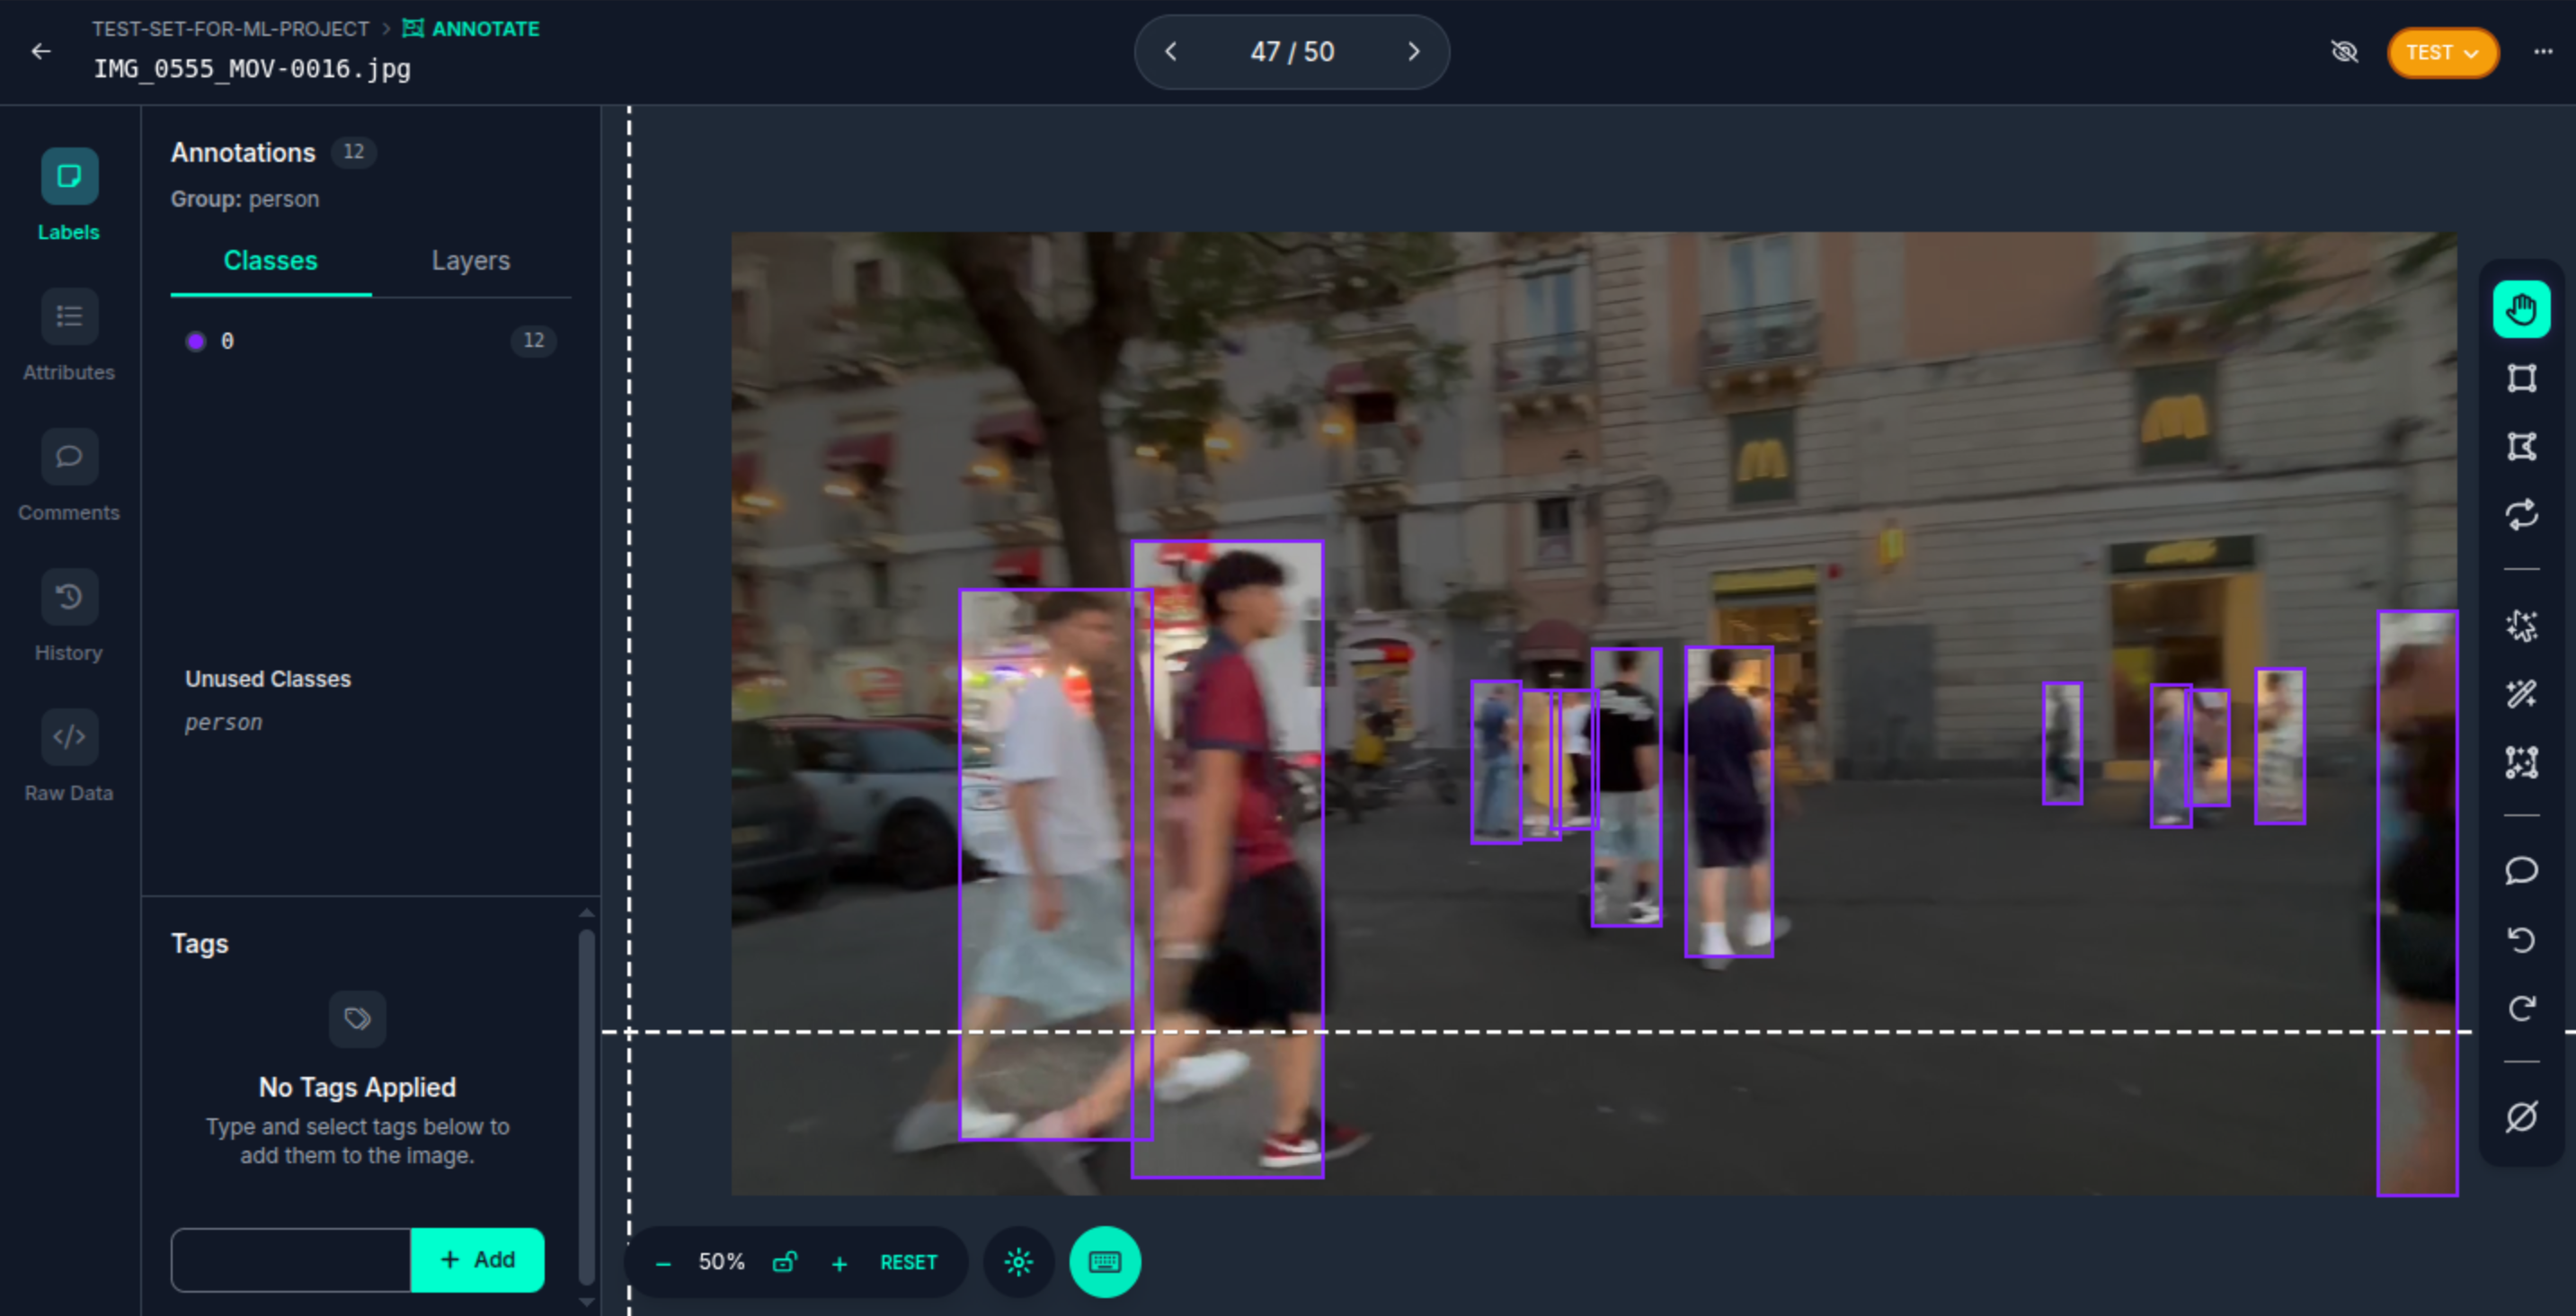
\includegraphics[width=0.90\textwidth]{./img/roboflow-label-example.png}
    \caption{Esempio di labelling con Roboflow}
    \label{fig:roboflow-labelling}
\end{figure}

\begin{figure}[H]
    \centering
    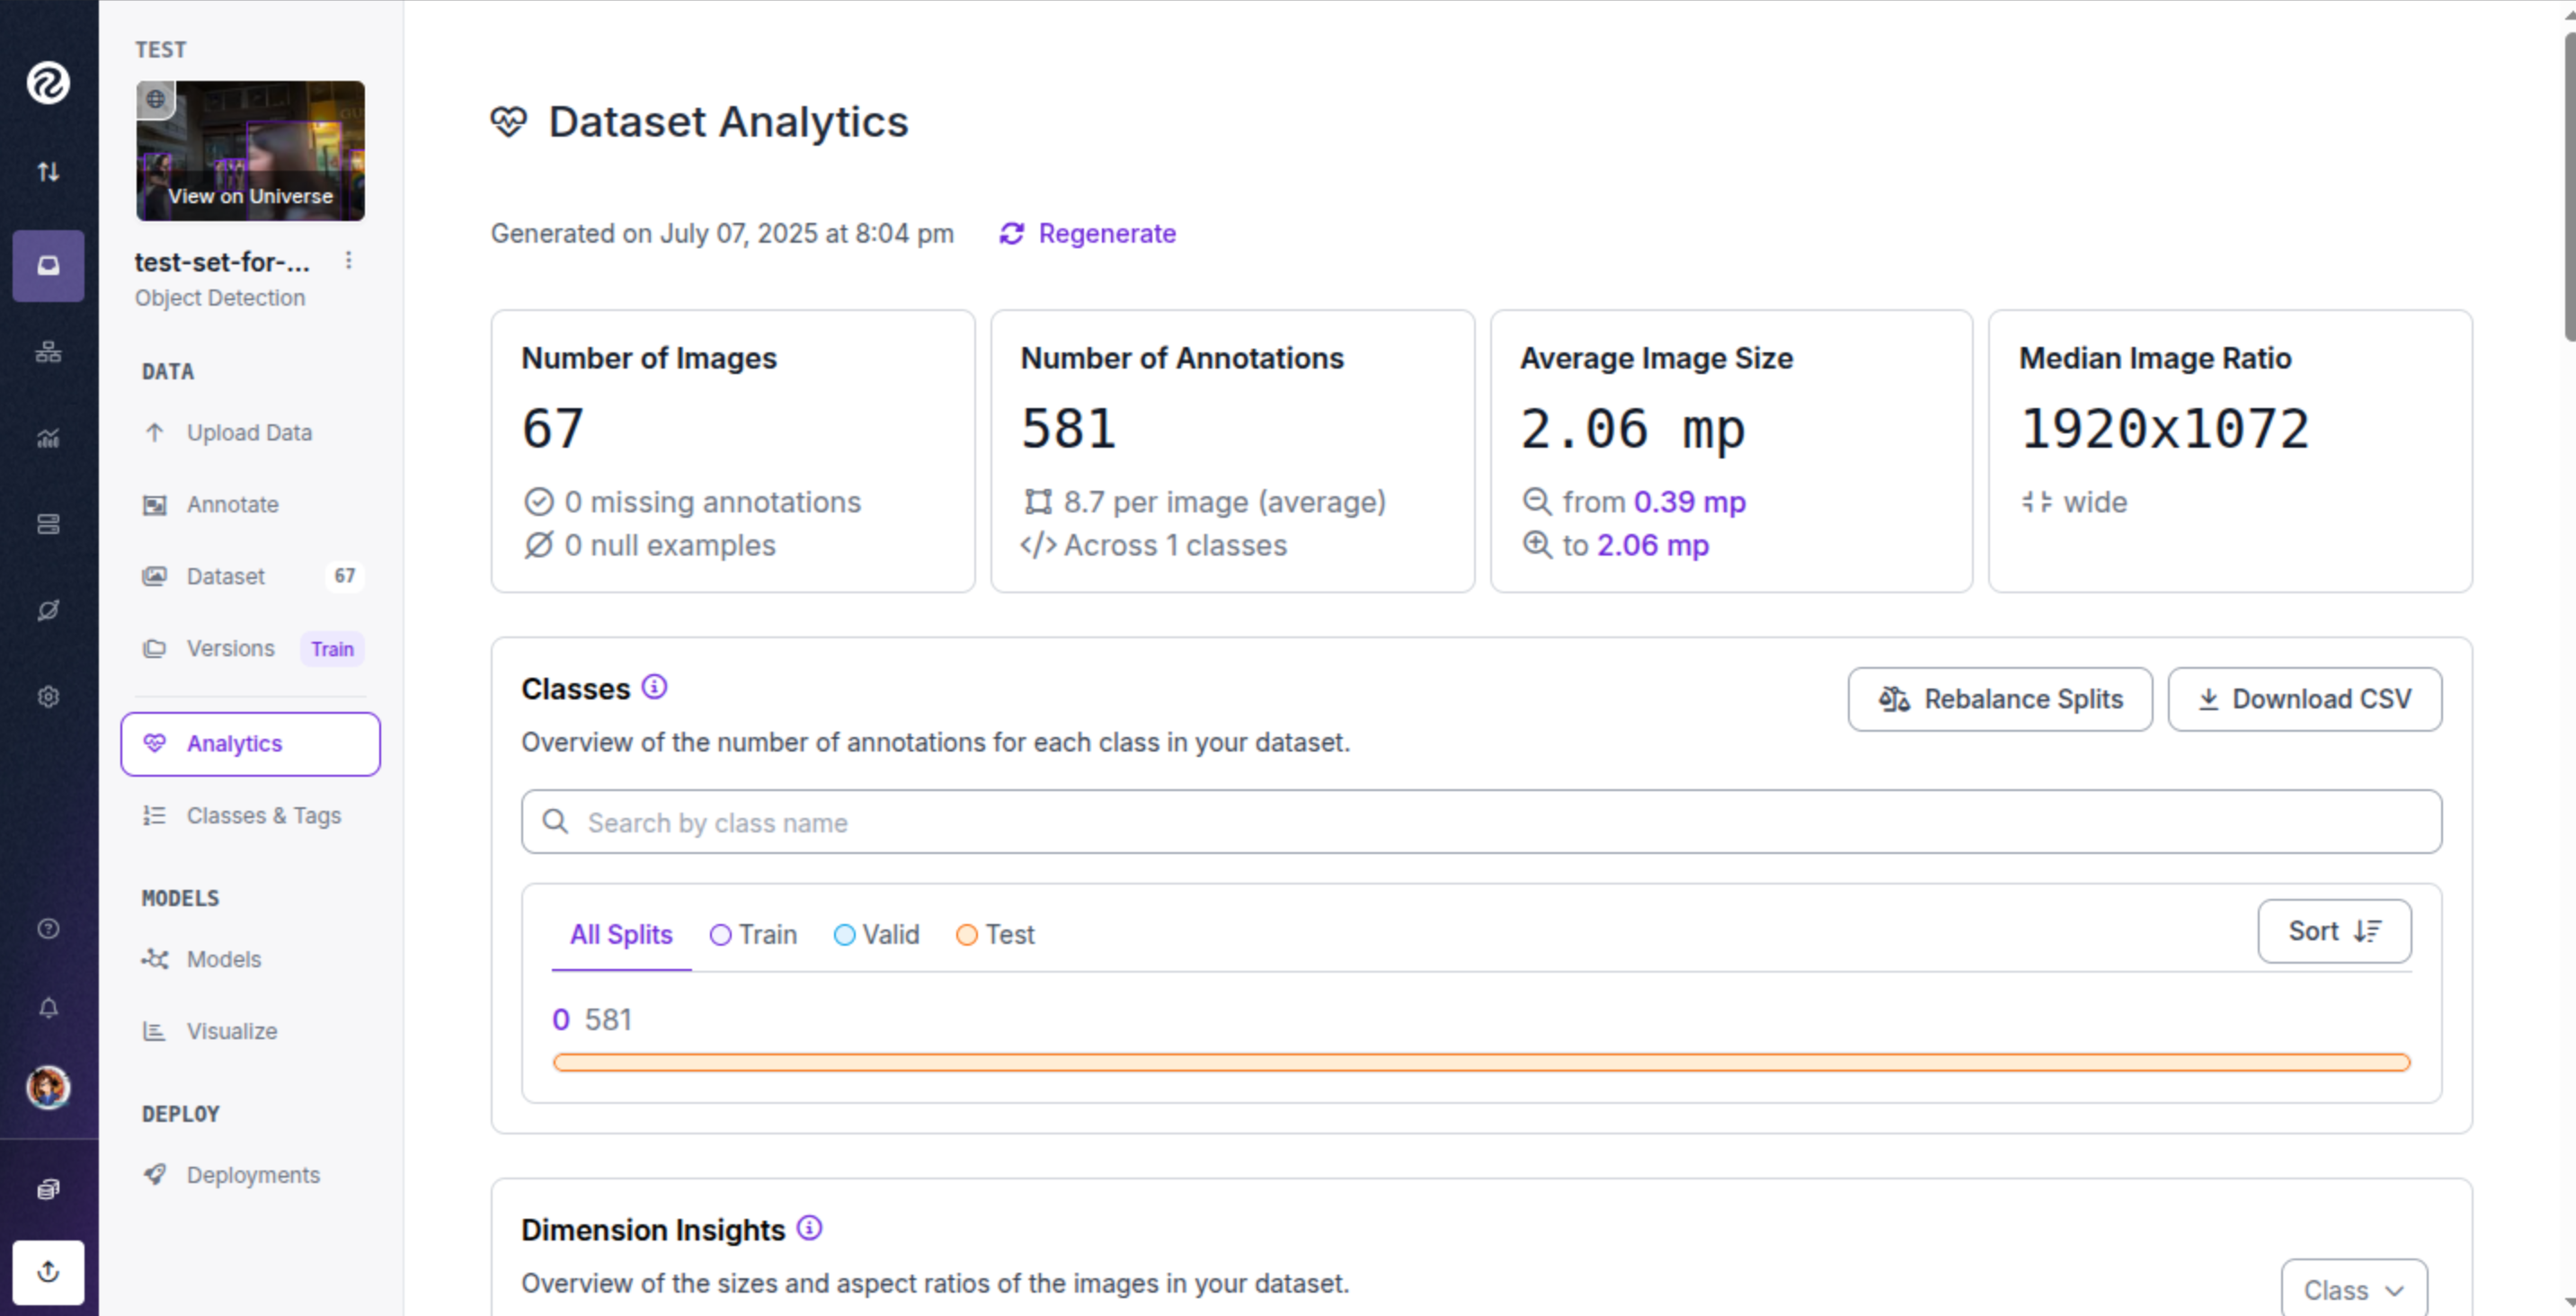
\includegraphics[width=0.90\textwidth]{./img/roboflow-test-set.png}
    \caption{Statistiche sul test set calcolate su Roboflow}
    \label{fig:roboflow-test-set}
\end{figure}

\subsubsection{Dati di esempio del test set}
Per poter comprendere meglio la tipologia dei frame utilizzati come test set, sono di seguito riportate un'immagine di esempio con la rispettiva \textbf{ground truth}: le reali etichette annotate mediante Roboflow.

\begin{figure}[H]
    \centering
    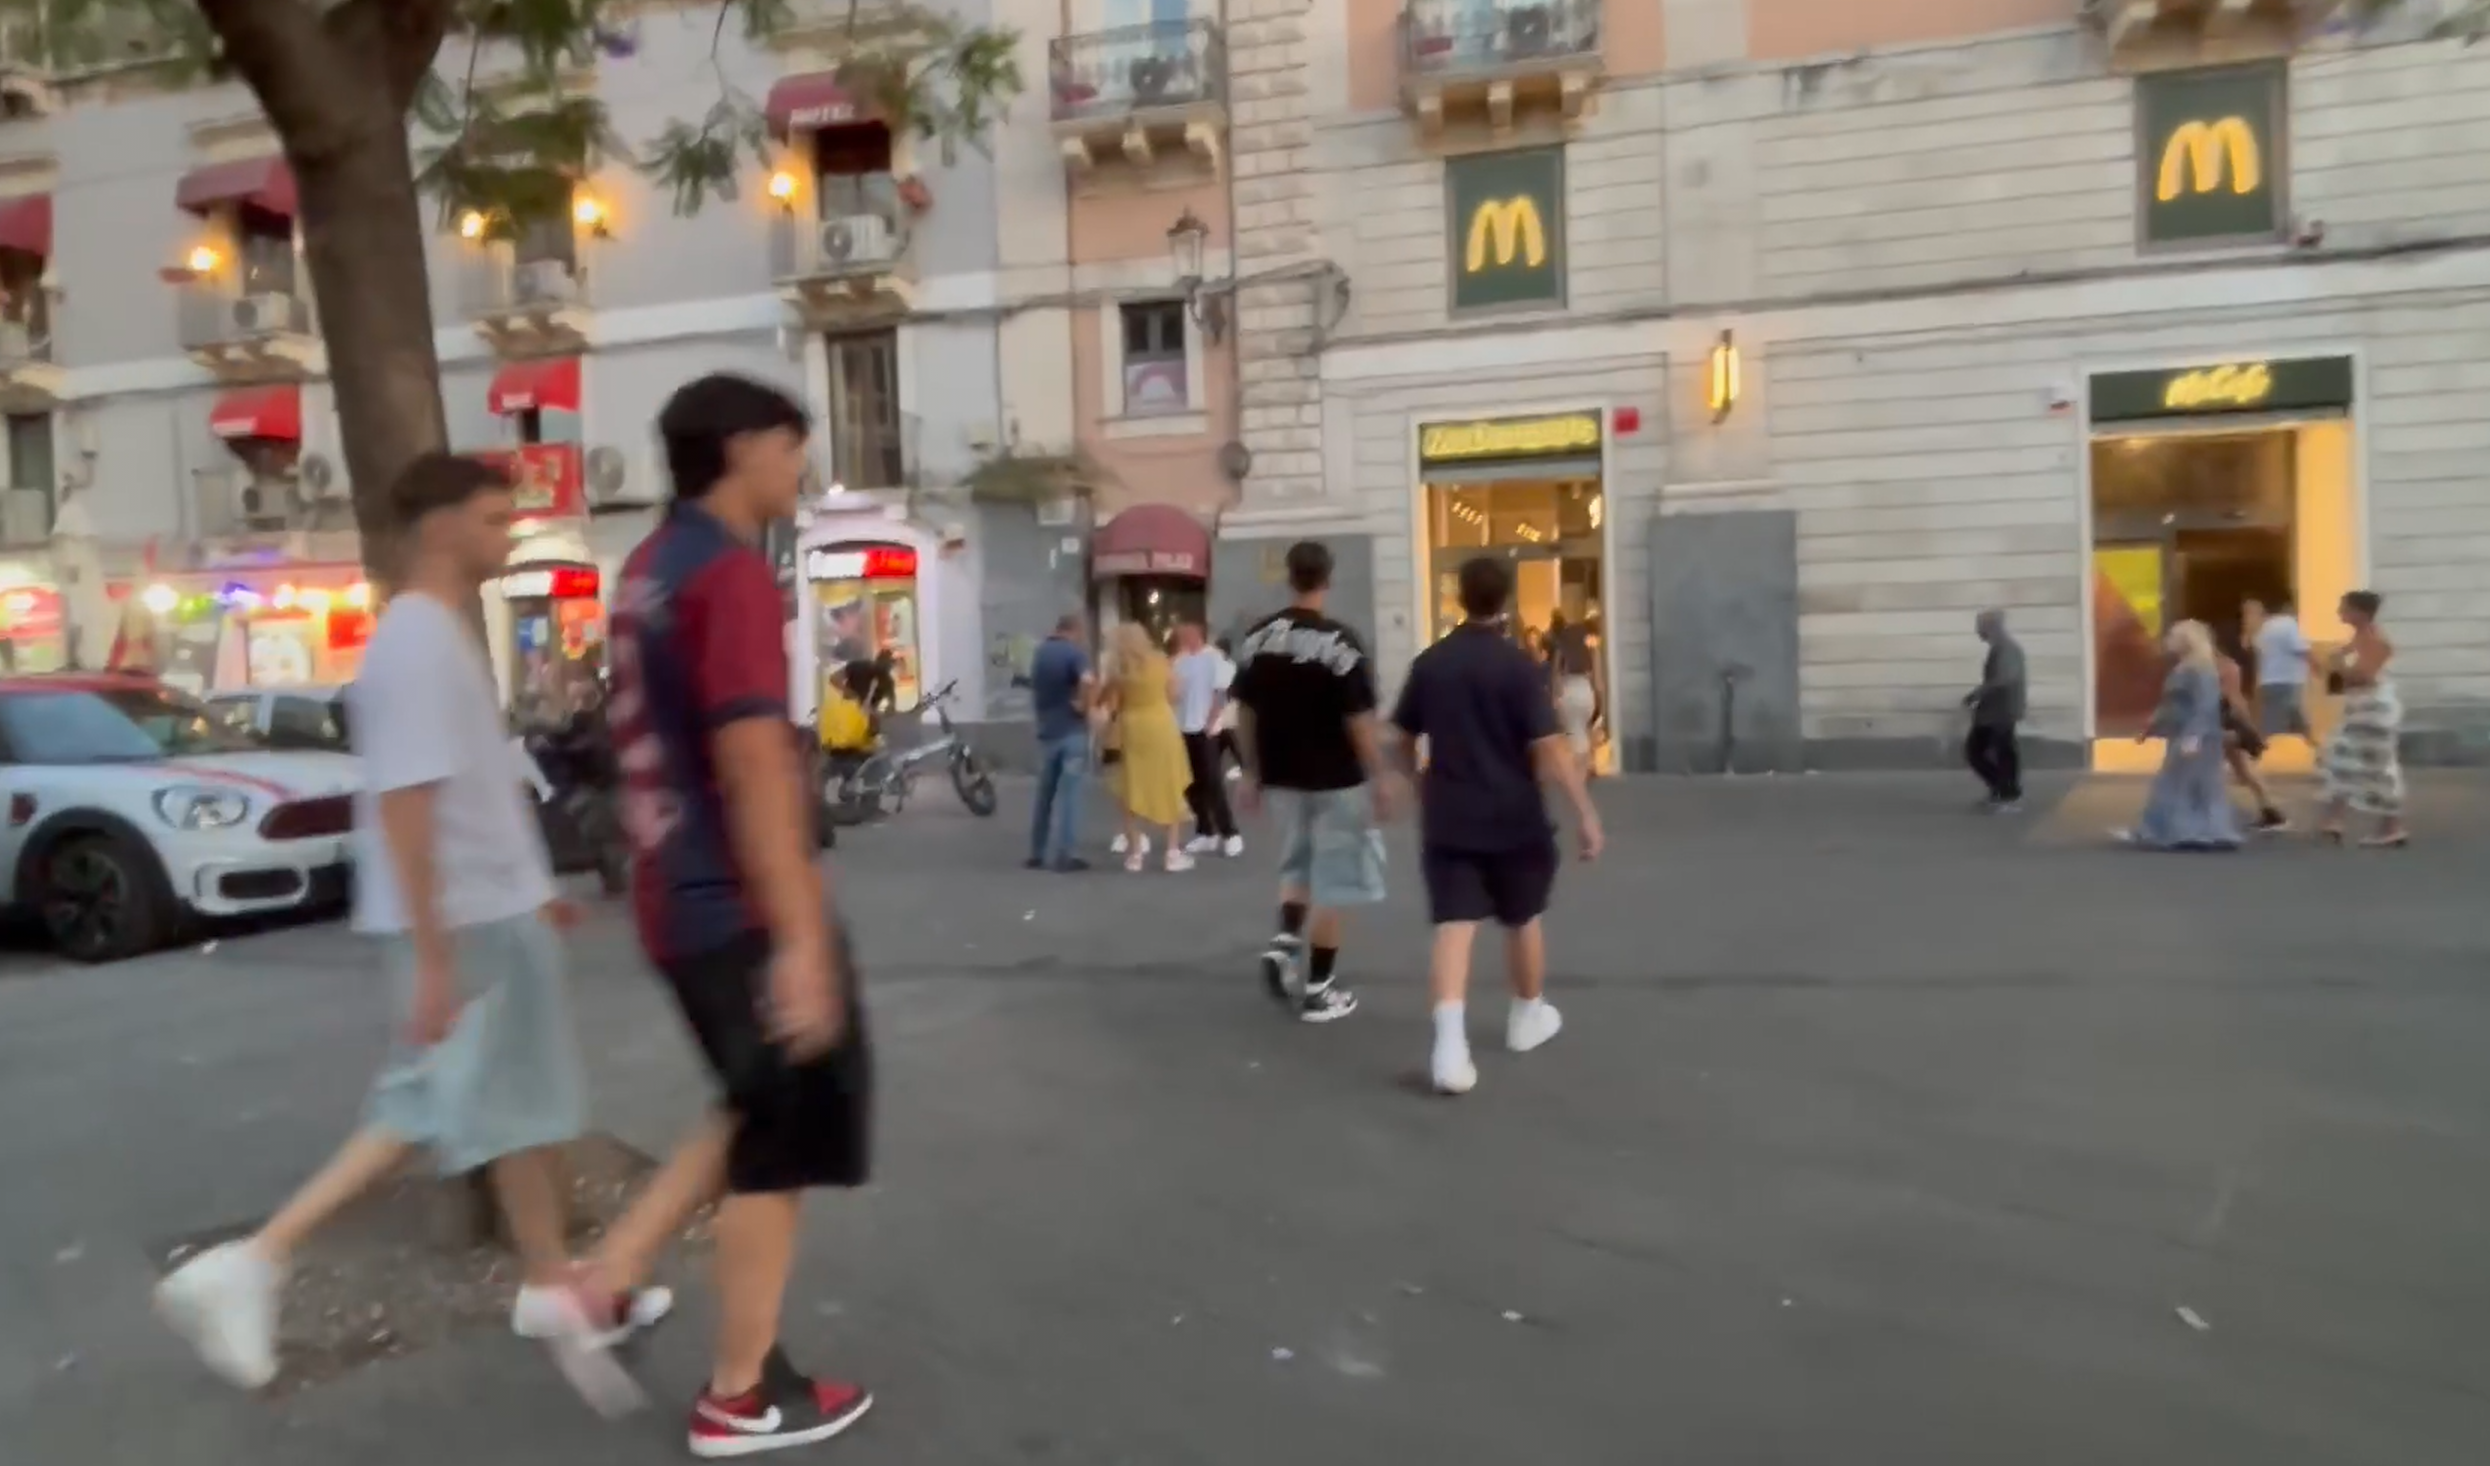
\includegraphics[width=1.00\textwidth]{./img/test-without-ground-truth.png}
    \caption{Frame del test set senza ground-truth}
    \label{fig:roboflow-test-set-no-gt}
\end{figure}

\begin{figure}[H]
    \centering
    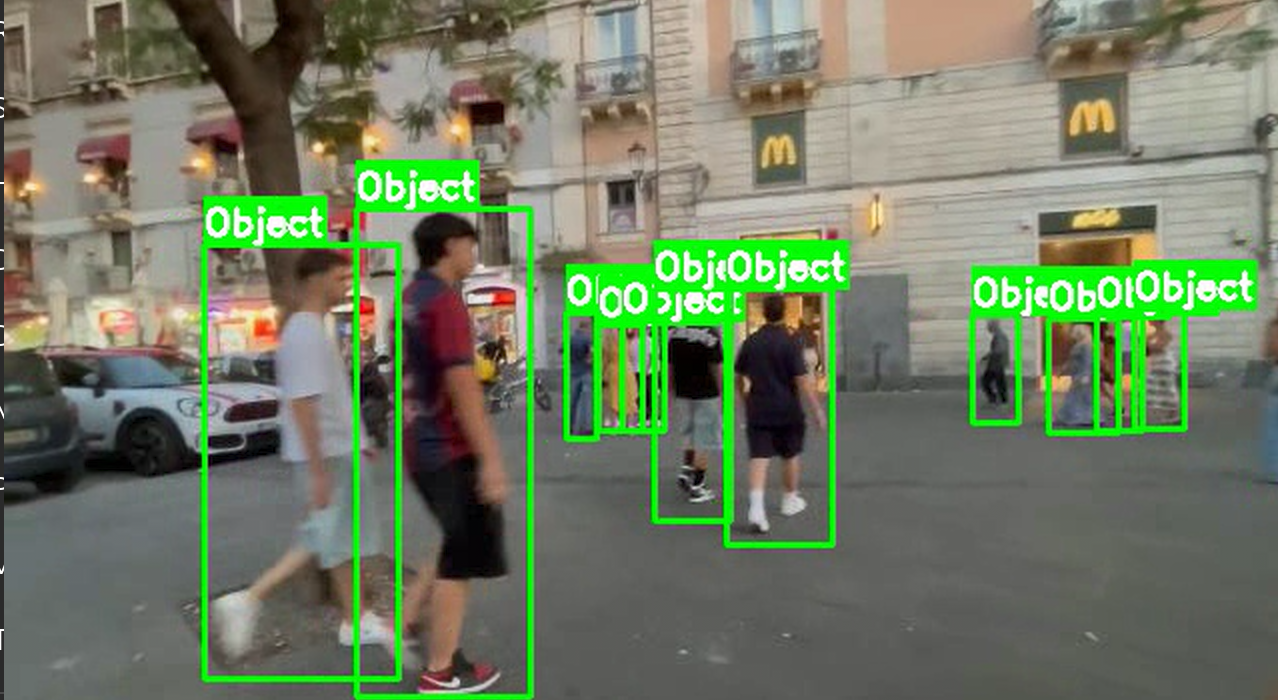
\includegraphics[width=1.00\textwidth]{./img/ground-truth-test.png}
    \caption{Frame del test set con ground-truth}
    \label{fig:roboflow-test-set-with-gt}
\end{figure}

\subsection{Pre-processing dei dataset}
Sono state necessarie diverse operazioni di pre-processing su entrambi i dataset per poter ottenere i miglior risultati possibili in termini di prestazioni e qualità nel training e nel test set dei modelli.\\
Le principali operazioni di pre-processing sui dataset sono:
\begin{itemize}
    \item \textbf{Resize} a dimensioni 640x640, ovvero la dimensione consigliata nei modelli YOLO.
    \item \textbf{Re-mapping dei Class-ID}. Per poter gestire al meglio la classe \textit{pedestrians} all'interno dei modelli è stato necessario rimuovere le righe inerenti a delle classi (1, 2, 3, 5, 6, 7) poiché non rappresentavano pedoni o persone; inoltre è stato necessario convertire le classi 4 e 8 in classi 0. Quest'ultima è la classe che identifica correttamente un pedone. Nel caso particolare del formato COCO JSON la classe 0 è solitamente associata al \textit{background}, pertanto in questo caso verrà associata al pedone la classe 1. 
\end{itemize}
La seconda operazione, il re-mapping, è stata effettuata utilizzando degli script Python per rendere il tutto più rapido ed automatico. Di seguito è possibile visualizzarne il codice sia per il formato YOLO che per il formato COCO JSON necessario per il modello Faster R-CNN.

\begin{lstlisting}[language=Python, caption={Esempio di codice per il remapping del formato YOLO}, label={lst:remapping-yolo}]
import sys
import os
import argparse
from pathlib import Path

def convert_yolo_annotations(input_file):    
    converted_lines = 0
    removed_lines = 0
    output_lines = []
    
    # Leggi il file di input
    with open(input_file, 'r', encoding='utf-8') as f:
        lines = f.readlines()
    
    for line_num, line in enumerate(lines, 1):
        line = line.strip()
        
        # Salta righe vuote
        if not line:
            continue
            
        # Dividi la riga in componenti
        parts = line.split()
        
        try:
            class_id = int(parts[0])
        except ValueError:
            print(f"AttenzioneRigaConClasseIDnonValido")
            continue
        
        # Applica le regole di conversione
        if class_id in [4, 8]:
            # Converte classe 4 e 8 -> classe 0
            parts[0] = '0'
            output_lines.append(' '.join(parts))
            converted_lines += 1
            
        elif class_id == 0:
            # Mantiene classe 0 invariata
            output_lines.append(line)
            
        elif class_id in [1, 2, 3, 5, 6, 7]:
            # Rimuove le righe con queste classi
            removed_lines += 1
    

    # Scrivi il file di output
    with open(input_file, 'w', encoding='utf-8') as f:
        for line in output_lines:
            f.write(line + '\n')
    
    return converted_lines, removed_lines


def process_directory(directory_path, recursive=False):
    directory = Path(directory_path)
    
    # Trova tutti i file .txt
    if recursive:
        txt_files = list(directory.rglob("*.txt"))
    else:
        txt_files = list(directory.glob("*.txt"))
    
    if not txt_files:
        print(f"NessunFileTrovato")
        return
    
    total_converted = 0
    total_removed = 0
    processed_files = 0
    
    for txt_file in txt_files:
        try:
            print(f"Processando:{txt_file}")
            converted, removed = convert_yolo
            _annotations(str(txt_file))
            
            total_converted += converted
            total_removed += removed
            processed_files += 1
            
            if converted > 0 or removed > 0:
                print(f"-Convertite:{converted}-righe-(4,8->0)")
                print(f"-Rimosse:{removed}-
righe-(classi--1,2,3,5,6,7)")
                
        except Exception as e:
            print(f"Errore:{e}")
    
\end{lstlisting}

\begin{lstlisting}[language=Python, caption={Esempio di codice per il remapping del formato COCO JSON}, label={lst:remapping-coco}]
import json
from pathlib import Path

def convert_annotations_inplace(json_file):
    # Leggi il file JSON
    with open(json_file, 'r', encoding='utf-8') as f:
        data = json.load(f)
    
    # ID delle categorie da eliminare e convertire
    categories_to_remove = {2, 3, 4, 6, 7, 8}
    categories_to_convert = {5, 9}
    
    # Statistiche iniziali
    original_annotations = len(data['annotations'])

    # 1. Filtra e converti le annotazioni
    filtered_annotations = []
    for annotation in data['annotations']:
        category_id = annotation['category_id']
        
        # Salta le annotazioni da eliminare
        if category_id in categories_to_remove:
            continue
        
        # Converti category_id 5 e 9 in 1
        if category_id in categories_to_convert:
            annotation['category_id'] = 1
        
        filtered_annotations.append(annotation)
    
    data['annotations'] = filtered_annotations
    
    # 2. Aggiorna le categorie
    new_categories = []
    for category in data['categories']:
        cat_id = category['id']
        
        # Salta le categorie da rimuovere
        if cat_id in categories_to_remove:
            continue
        
        # Aggiorna la categoria 1 per riflettere la fusione
        if cat_id == 1:
            category['name'] = "pedestrian"
            category['supercategory'] = "pedestrians-"
        
        # Mantieni solo le categorie necessarie
        if cat_id in {0, 1}:
            new_categories.append(category)
    
    data['categories'] = new_categories
    
    
    # Salva il file modificato
    with open(json_file, 'w', encoding='utf-8') as f:
        json.dump(data, f, indent=2, ensure_ascii=False)
    
    # Statistiche finali
    print(f" Annotazioni:{original_annotations}
->{len(data['annotations'])}")
    print(f"Categorie:{len(new_categories)}")
\end{lstlisting}

\section{Metodi}
\subsection{Funzionamento YOLO}
Il principio fondamentale di YOLO risiede nella sua strategia di suddividere l'immagine in una griglia. Ogni cella di questa griglia è incaricata di prevedere la presenza di un oggetto il cui centro ricade al suo interno. Per ogni cella, il modello genera delle previsioni relative ai riquadri di delimitazione (bounding box), al grado di certezza della previsione (punteggio di confidenza) e alle probabilità delle diverse classi di oggetti. Questa architettura integrata consente a YOLO di raggiungere velocità di elaborazione elevate, rendendolo particolarmente adatto per applicazioni che richiedono risposte immediate. Le successive evoluzioni di YOLO hanno costantemente affinato questo meccanismo di base, migliorando l'accuratezza senza compromettere la rapidità.\\
Di seguito, verranno spiegati in dettaglio i meccanismi specifici di funzionamento di YOLO.

\subsubsection{Residual block} 
Un residual block è un componente utilizzato per facilitare l’addestramento di reti molto profonde, ampiamente utilizzato nelle architetture YOLO moderne. Il concetto chiave è la skip connection: l’output di un gruppo di layer convoluzionali F(x) viene sommato all’input originale x, realizzando un collegamento identitario diretto. Matematicamente, il blocco residuo può essere rappresentato come: 

\begin{center}
$y = F(x)+x$,    
\end{center}
dove $x$ è l’input del blocco, $F(x)$ rappresenta la trasformazione appresa e $y$ l’output. Questa formulazione preserva il gradiente durante il backpropagation anche in reti molto profonde, mitigando problemi di vanishing gradient. In sintesi, i blocchi residui migliorano la propagazione delle informazioni e la stabilità del training nei modelli YOLO, consentendo reti più profonde e prestazioni migliori grazie alla riutilizzazione dei segnali a vari livelli della rete.

\begin{figure}[H]
    \centering
    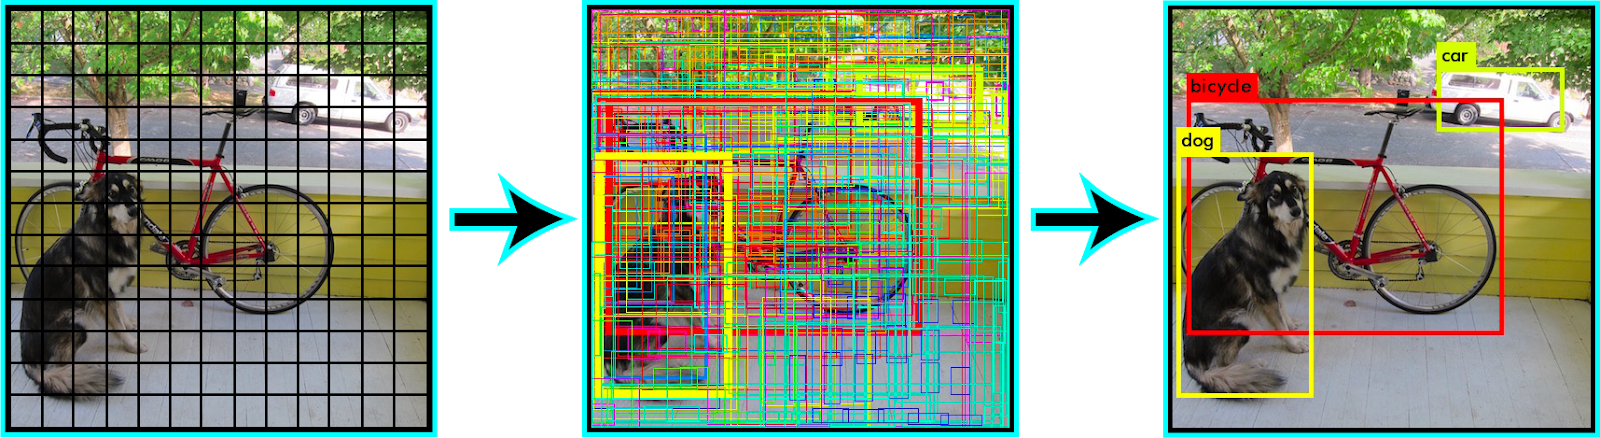
\includegraphics[width=1.1\textwidth]{./img/residual-block-img.png}
    \caption{Esempio di Residual Block}
    \label{fig:residual-block-example}
\end{figure}


\subsubsection{Bounding box regression} 

Rappresenta il cuore di un detector YOLO. Data un’immagine, questa può contenere un numero variabile di oggetti, ciascuno dei quali viene rappresentato da una bounding box predetta dal modello. YOLO ne determina i valori tramite un modulo di regressione nel seguente formato come segue: 

\begin{center}
$Y = [pc, bx, by, bh, bw, c1, ... , cn]$.    
\end{center}

dove: 
\begin{itemize}
\item pc:  indica la probabilità che un oggetto sia presente, 
\item bx, by: sono le coordinate normalizzate del centro,
\item bw, bh: larghezza e altezza,
\item $c_i$: sono le probabilità di classe.
\end{itemize}
Ogni bounding box è comunemente rappresentata dal punto centrale ($x$, $y$), dalla larghezza $w$ e dall’altezza $h$ del riquadro rispetto all’immagine. I modelli YOLO originari (v1-v3) utilizzavano anchor boxes come riferimenti predefiniti di forma: la rete in uscita prediceva delle quantità $t_x$, $t_y$, $t_w$, $t_h$ che venivano poi trasformate nelle coordinate finali del box aggiustando l’ancora assegnata.\\ 
Durante l’addestramento, YOLO confronta ogni box predetto con i ground truth corrispondenti usando una loss multicomponente. Ad esempio in Yolov8 si ha la combinazione di CIoU (Complete IoU loss)+ Distribution Focal Loss.
Questi accorgimenti assicurano che la bounding box regression produca riquadri più accurati e stabili durante il training e inferenza, tenendo conto non solo dell’errore assoluto sulle coordinate ma anche della misura di overlap e dell’allineamento geometrico tra predizione e ground truth.

\begin{figure}[H]
    \centering
    \includegraphics[width=0.60\textwidth]{./img/bounding-box-img.png}
    \caption{Esempio di Bounding Box}
    \label{fig:bounding-box-example}
\end{figure}


\subsubsection{Intersection Over the Union}

L’Intersection over Union (IoU) è la metrica standard per valutare la sovrapposizione tra due bounding box, ed è cruciale sia in fase di training che di valutazione dei modelli YOLO. Data una bounding box predetta $B_p$ e la bounding box ground truth $B_{gt}$, l’IoU è definita come il rapporto tra l’area di intersezione e l’area di unione dei due riquadri:

\begin{center}
\[
\mathrm{IoU}(B_p, B_{gt}) = \frac{\mathrm{Area}(B_p \cap B_{gt})}{\mathrm{Area}(B_p \cup B_{gt})}
\]
\end{center}
In particolare, IoU varia da 0 (inteso come nessuna intersezione) a 1 (inteso come sovrapposizione perfetta). \\
Durante la fase di addestramento, questa viene utilizzata per determinare quale anchor (o cella) è responsabile di predire un dato oggetto. Mentre, per la fase di valutazione, l'IoU viene impiegato per decidere se una predizione è considerata un True Positive: ad esempio una detection è ritenuta corretta se l’IoU con il ground truth supera una certa soglia (generalmente 0.5). Inoltre, molte funzioni di loss avanzate (come GIoU, DIoU, CIoU, SIoU) estendono o pesano la metrica IoU per guidare la regressione delle box in modo più efficace. \\
Infine, nel contesto della NMS (Non-Maximum Suppression), l’IoU è il criterio con cui si valuta la ridondanza di due predizioni: se due box predetti per lo stesso oggetto hanno un IoU elevato, uno dei due verrà soppresso.

\begin{figure}[H]
    \centering
    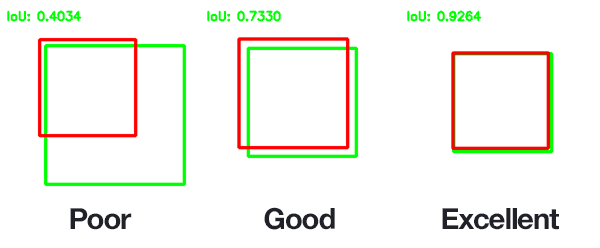
\includegraphics[width=0.90\textwidth]{./img/iou-img.png}
    \caption{Esempio di Intersection Over Union}
    \label{fig:iou-example}
\end{figure}


\subsubsection{Non-Maximum Suppression} 

E' una procedura di post-processing utilizzata tradizionalmente dai modelli YOLO (e dai detector in generale) per eliminare le predizioni duplicate relative allo stesso oggetto. \\
Il suo impiego risulta necessario poiché le bounding box non sopresse nel passaggio precedente, possono essere molto vicine tra loro e creare rumore.  \\
In pratica, per ciascuna classe si ordinano le bounding box predette per punteggio di confidenza; si prende la box con confidenza più alta e la si emette come rilevazione finale, quindi si sopprimono tutte le altre box che hanno con essa un IoU superiore a una certa soglia (di solito 0.5). Si ripete poi il processo con la successiva box rimanente in ordine di score, fino ad esaurire le predizioni
Questo semplice procedimento garantisce che per ogni oggetto venga riportata idealmente una sola bounding box. \\
Tuttavia, è necessario portare l'attenzione su  YOLOv10 che rappresenta un cambio di paradigma poiché, tramite la strategia di consistent one-to-one assignment in training. Quest'ultimo elimina la necessità di NMS poiché la rete impara a produrre al massimo una box per oggetto. Ogni oggetto viene assegnato alla migliore predizione (e non a molteplici anchor come avveniva prima), riducendo drasticamente le duplicazioni in output. Questo approccio NMS-free non solo semplifica la pipeline end-to-end, ma riduce anche la latenza e migliora potenzialmente la precisione in scenari affollati, dove NMS talvolta poteva sopprimere rilevazioni valide. \\
In conclusione, si ritiene comunque corretto attenzionare la Non-Maximum Suppression poiché è stata a lungo un elemento fondamentale nell’oggettistica di YOLO per ottenere output puliti e privi di duplicati; le ultime evoluzioni della famiglia mirano però a incorporarne gli effetti direttamente nel processo di training, rendendo il modello end-to-end senza post-processing esplicito.

\begin{figure}[H]
    \centering
    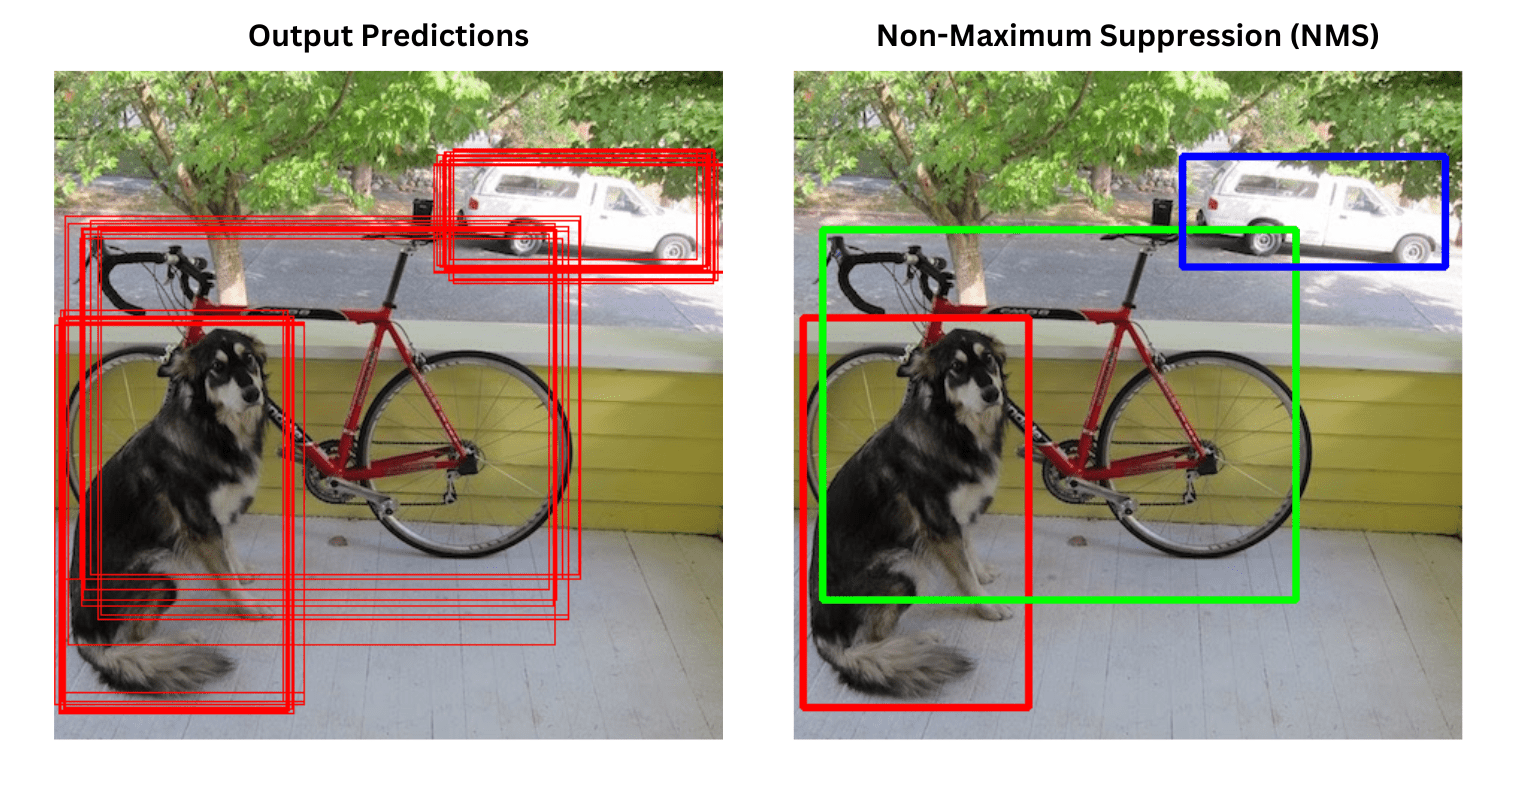
\includegraphics[width=1.0\textwidth]{./img/nms-img.png}
    \caption{Funzionamento di NMS}
    \label{fig:nms-example}
\end{figure}

\subsection{Funzionamento Faster R-CNN}
Faster R-CNN si distingue per la sua architettura a due stadi, che le permette di raggiungere un'elevata precisione nella localizzazione e classificazione degli oggetti. Opera attraverso un processo a due fasi distinte e consecutive, che insieme garantiscono un'elevata precisione nell'identificazione e classificazione degli oggetti. \\
Di seguito si entrerà nei dettagli del suo funzionamento.

\subsubsection{Feature Extraction}
Il primo stadio di Faster R-CNN si concentra sull'identificazione delle aree dell'immagine che potrebbero contenere un oggetto. Inizialmente, l'immagine viene processata da una \textit{backbone network}, ovvero una rete neurale convoluzionale profonda. Quest'ultima viene spesso pre-addestrata su vasti dataset di immagini come ImageNet; questo processo permette di imparare il riconoscimento di un'ampia varietà di caratteristiche visive. La backbone, dunque, estrae una mappa di caratteristiche ad alto livello dall'intera immagine. \\
Nel contesto di studi come il presente, l'utilizzo di \textbf{Resnet50} come backbone network per Faster R-CNN è una scelta comune. Resnet50 (\textbf{Residual Network con 50 strati}) è una CNN profonda e molto efficiente, rinomata per la sua capacità di superare il \textit{vanishing gradient problem} (un ostacolo comune nelle reti molto profonde) grazie all'introduzione di connessioni residue (\textit{skip connections}). Queste connessioni permettono ai gradienti di fluire più liberamente attraverso la rete, facilitando l'addestramento di modelli molto profondi e consentendo a Resnet50 di apprendere rappresentazioni complesse e ricche, fondamentali per il riconoscimento accurato degli oggetti.

\subsubsection{Region Proposal Network - RPN}
Successivamente, entra in gioco il \textbf{Region Proposal Network} (RPN). L'RPN è una piccola rete neurale che scansiona la mappa di caratteristiche estratta. Il suo compito non è ancora quello di classificare gli oggetti, ma di generare una serie di proposte di regione (\textit{Region Proposals}), ovvero dei bounding box preliminari che indicano dove è probabile che sia presente un oggetto. L'RPN valuta ogni potenziale area e assegna un punteggio di oggettività, indicando quanto è probabile che quell'area contenga qualcosa di interessante (un oggetto) piuttosto che semplice sfondo. Questo processo è cruciale perché riduce drasticamente il numero di aree da analizzare nel dettaglio, concentrando l'attenzione del modello solo sulle porzioni più promettenti dell'immagine.

\begin{figure}[H]
    \centering
    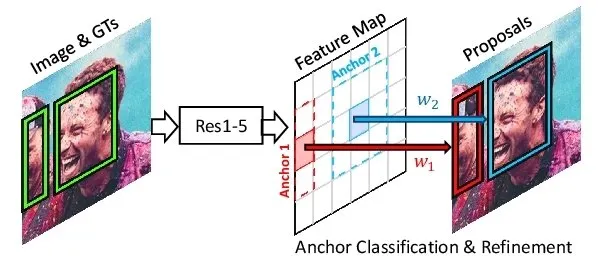
\includegraphics[width=1.00\textwidth]{./img/rpn-example.png}
    \caption{Esempio di Region Proposal Network}
    \label{fig:rpn-example}
\end{figure}


\subsubsection{Classificazione e Refinement (RoI Pooling)}
Una volta che l'RPN ha generato le sue proposte di regione, queste vengono passate al secondo stadio per un'analisi ancora più approfondita. Per prima cosa, un meccanismo chiamato \textbf{RoI Pooling} (\textit{Region of Interest Pooling}, o \textit{RoI Align} nelle versioni più recenti per una maggiore precisione) standardizza le dimensioni di tutte le proposte di regione, indipendentemente dalla loro dimensione originale. Questo è necessario perché i successivi strati di classificazione e regressione richiedono input di dimensione fissa.
Le regioni standardizzate vengono poi alimentate a due "teste" parallele:
\begin{itemize}
\item \textbf{Classificatore:} Una rete neurale che prende ogni proposta di regione e ne determina la classe specifica (ad esempio, "persona", "veicolo", "sfondo"). È qui che il modello decide cosa c'è all'interno del bounding box.
\item \textbf{Regressore del Bounding Box:} Un'altra rete neurale che affina le coordinate del bounding box generato dall'RPN. Questo passaggio è fondamentale per rendere il riquadro il più preciso possibile, adattandolo perfettamente all'oggetto rilevato.
\end{itemize} 

\begin{figure}[H]
    \centering
    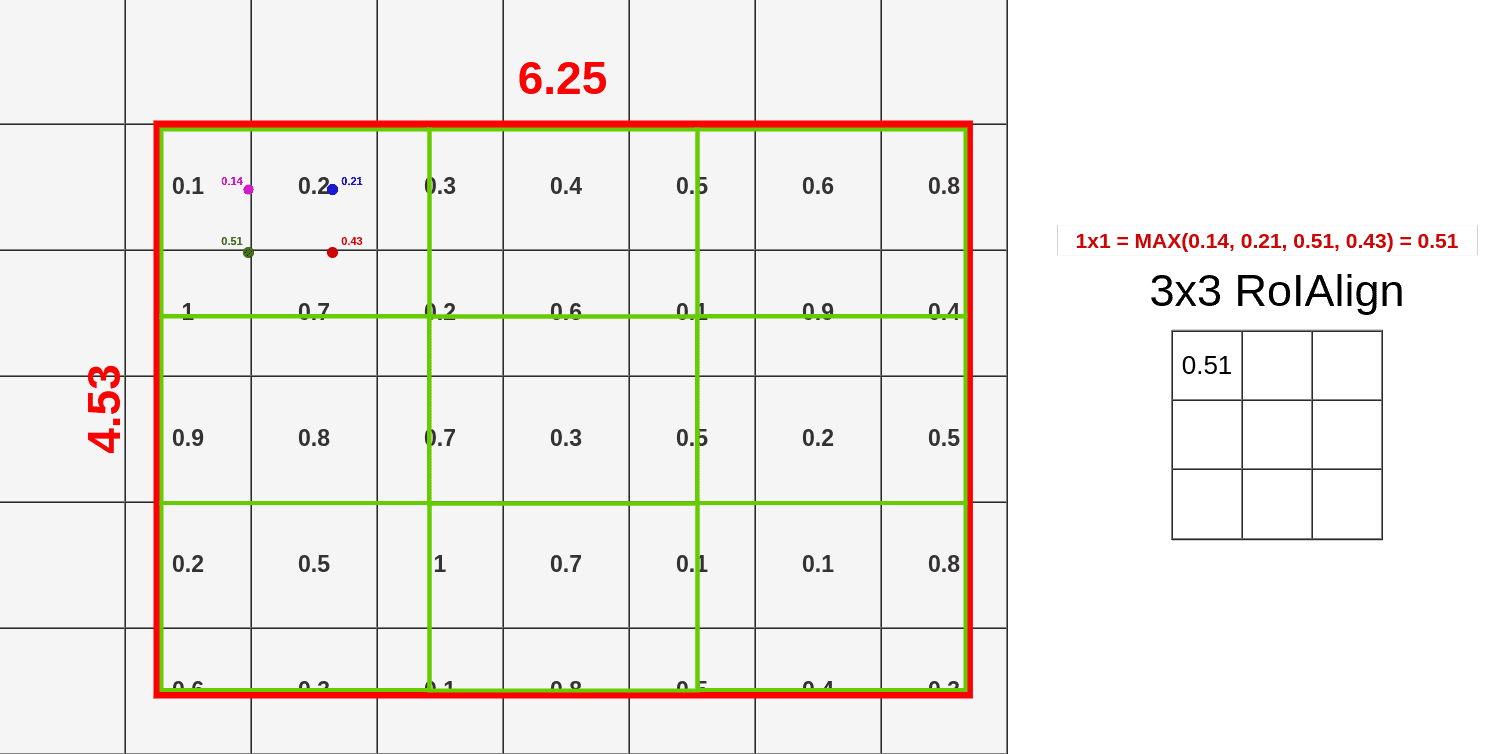
\includegraphics[width=1.00\textwidth]{./img/roi-align-img.png}
    \caption{Esempio di RoI Align}
    \label{fig:roi-example}
\end{figure}


\section{Valutazione del modello}
Nel presente capitolo, vengono elencate e discusse le metriche di valutazione, sia in termini di valori numerici che di rappresentazioni grafiche, utilizzate per analizzare le performance dei modelli di Object Detection impiegati, inclusi i modelli YOLO e Faster R-CNN.

\subsection{Metriche di valutazione}
Le metriche utilizzate per i benchmarking del presente progetto sono alcune delle metriche più utilizzate nell’ambito della valutazione di algoritmi di Object Detection. In particolare, sono state usate le seguenti metriche:

\begin{itemize}
    \item \textbf{Precision:} misura la proporzione di predizioni positive corrette rispetto a tutte le predizioni positive effettuate dal modello. Viene definita come il rapporto tra i True Positive e la somma dei True Positive e False Positive:
    $$ \text{Precision} = \frac{\text{TruePositive}}{\text{TruePositive} + \text{FalsePositive}} $$

    \item \textbf{Recall:} detta anche ”sensitivity”, misura la proporzione di rilevamenti positivi corretti rispetto a tutte le istanze effettivamente positive. Viene definita come il rapporto tra i True Positive e la somma dei True Positive e False Negative:
    $$ \text{\textit{Recall}} = \frac{\text{\textit{TruePositive}}}{\text{\textit{TruePositive}} + \text{\textit{FalseNegative}}} $$

    \item \textbf{F1-score:} è una metrica che tiene conto sia della precision che della recall. È molto utile nel caso in cui si vogliano bilanciare precision e recall, in quanto penalizza valori fortemente negativi di precision o recall. Viene calcolata come una media armonica tra precision e recall:
    $$ \text{\textit{F1}} = 2 \times \frac{\text{\textit{Precision}} \times \text{\textit{Recall}}}{\text{\textit{Precision}} + \text{\textit{Recall}}} $$

    \item \textbf{Valore di confidenza:} detto anche confidence score, è un numero compreso tra 0 e 1, associato ad ogni predizione effettuata da un modello di Machine Learning, che indica la probabilità che quest’ultima sia corretta.
    Nel caso di un modello di Object Detection come YOLO, essa indica la probabilità che la classe associata dal modello all’oggetto individuato sia corretta.

    \item \textbf{Curva Precision-Recall:} grafico utilizzato per valutare le prestazioni di un modello. Questa curva mostra la variazione della precision in funzione della recall.

    \item \textbf{Average Precision:} misura l’area al di sotto della curva precision-recall. Viene calcolata come segue:
    $$ \text{\textit{AP}} = \int_0^1 p(r)dr $$

    \item \textbf{Intersection over Union (IoU):} è una metrica di valutazione usata per misurare l’accuracy di un modello di Object Detection. Al fine di calcolarne il valore, si devono considerare:
    \begin{itemize}
        \item Bounding box ground-truth
        \item Bounding box predetti
    \end{itemize}
    Come dice il nome stesso, è definita come il rapporto tra l’intersezione e l’unione tra l’area occupata dal bounding box reale e dal bounding box predetto. In altre parole, calcola il rapporto tra l’area di overlap tra i due bounding box e la loro unione:
    $$ \text{IoU} = \frac{\text{\textit{IntersectionArea}}}{\text{\textit{UnionArea}}} $$
    Nella pratica, la metrica IoU assume valori elevati nel momento in cui il bounding box predetto è quanto più uguale possibile al bounding box reale, sia in termini di dimensione che di posizione.

    \item \textbf{Mean Average Precision - mAP:} media delle AP calcolate su tutte le classi presenti nel dataset. Viene calcolata come segue:
    $$ \text{\textit{mAP}} = \frac{1}{N} \sum_{i=1}^{N} \text{AP}_i $$
    con $N$ numero di classi. Nel presente progetto saranno usate due varianti:
    \begin{itemize}
        \item \textbf{mAP50:} misura la mAP impostando una soglia di ”Intersection over Union (IoU)” pari a 0.5.
        \item \textbf{mAP75:} misura la mAP impostando una soglia di ”Intersection over Union (IoU)” pari a 0.75.
        \item \textbf{mAP50-95:} misura la mAP impostando una soglia minima di ”Intersection over Union (IoU)” pari a 0.5 e una soglia massima pari a 0.95.
    \end{itemize}
\end{itemize}

\subsection{Grafici}
I grafici usati ai fini della valutazione dei modelli addestrati sono i seguenti:

\begin{itemize}
    \item \textbf{Matrice di confusione:} è una tabella che mostra il numero di previsioni corrette e errate effettuate da un modello su un set di dati. Viene in genere utilizzato per valutare le prestazioni di un modello di classificazione binaria, ma può anche essere applicato a attività di classificazione multiclasse. In particolare, l’asse delle ascisse rappresenta le classi reali, mentre l’asse delle ordinate rappresenta le classi predette.
    Nel caso di un problema di classificazione binario, all’interno della matrice di confusione è possibile distinguere:
    \begin{itemize}
        \item Veri positivi (TP): il numero di esempi che sono stati previsti come positivi e sono effettivamente positivi.
        \item Veri negativi (TN): il numero di esempi che sono stati previsti come negativi e sono effettivamente negativi.
        \item Falsi positivi (FP): il numero di esempi previsti come positivi ma in realtà negativi.
        \item Falsi negativi (FN): il numero di esempi previsti come negativi ma in realtà positivi.
    \end{itemize}

\begin{figure}[H]
    \centering
    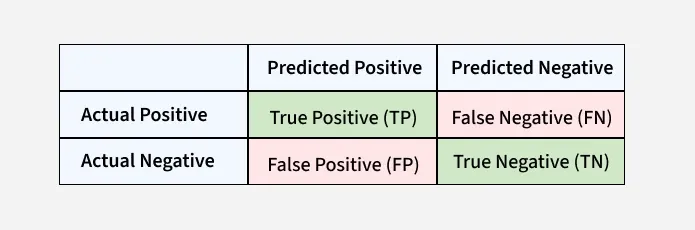
\includegraphics[width=1.00\textwidth]{./img/predicted_condition_2_.png}
    \caption{Esempio di matrice di confusione}
    \label{fig:confusion-matrix-example}
\end{figure}

    \item \textbf{Grafici che mostrano relazioni tra misure di valutazione e score di confidenza:} nella fase di valutazione del modello sono stati utilizzati grafici che mostrano come variano i valori assunti dalle metriche di valutazione al variare di una threshold sul valore di confidenza delle predizioni, ovvero vengono considerate valide esclusivamente le predizioni la cui confidenza è maggiore rispetto alla soglia impostata. Segue che maggiore è la soglia scelta, minore sarà il numero di predizioni considerate valide.
    \begin{itemize}
        \item \textbf{Precision-Confidence Curve:} è una rappresentazione visuale della relazione tra precision e confidenza. In particolare, rappresenta il valore di precision ottenuto per diverse threshold di valori di confidenza. In particolare, per valori elevati di soglia di confidenza, il modello risulterà molto preciso, in quanto, impostando una determinata soglia, sono considerate valide solo predizioni con valori di confidenza al di sopra di essa.
        \item \textbf{Recall-Confidence Curve:} è una rappresentazione visuale della relazione tra recall e confidenza. In particolare, mostra come varia la recall in funzione della variazione della soglia di confidenza. Utilizzando tale grafico, si nota come quando la threshold di confidenza diminuisce, più predizioni sono considerate valide.
        \item \textbf{F1-Confidence Curve:} è una rappresentazione visuale della relazione tra F1 score e confidenza. In particolare, mostra come varia il F1 score in funzione della variazione della soglia di confidenza. Un valore alto di F1 score indica performance migliori, e di conseguenza, la soglia di confidenza per cui si ottiene tale valore solitamente è la migliore per effettuare predizioni quanto più accurate possibile.
    \end{itemize}
\end{itemize}

\subsection{Loss functions}
Sono di seguito riportate le principali funzioni di loss analizzate. Esse in particolare riguardano sia la fase di training che la validazione.
Le principali sono le seguenti:

\begin{itemize}
    \item \textbf{train/box loss:} indica la loss legata alla localizzazione dei box durante il training.
    \item \textbf{train/cls loss:} indica la loss legata alle predizioni errate riguardanti le classi di appartenenza degli oggetti identificati, durante il training.
    \item \textbf{train/dfl loss:} indica la cosiddetta ”Distribution Focal Loss”, e riguarda principalmente la loss legata a predizioni errate del modello per istanze più ”complesse” e meno rappresentate all’interno del dataset, le quali sono ”pesate” maggiormente.
    \item \textbf{val/box loss:} come la train/box loss, ma riguarda stavolta il validation set.
    \item \textbf{val/cls loss:} come la train/cls loss, ma riguarda stavolta il validation set.
    \item \textbf{val/dfl loss:} come la train/dfl loss, ma riguarda stavolta il validation set.
\end{itemize}


\section{Fase di Training e Validazione}

Nella presente sezione vengono descritti gli aspetti principali delle fasi di training e validazione dei diversi modelli YOLO impiegati (\textbf{YOLOv8m}, \textbf{YOLOv10n}, \textbf{YOLOv11s}), utilizzando il dataset e le metriche di valutazione definiti nei capitoli precedenti. In particolare, verranno elencati i parametri di training adottati, i passi seguiti per effettuare il training e la validazione (inclusi i frammenti di codice utilizzati) e saranno mostrati i principali risultati attraverso grafici e tabelle.\\
Si assume che l’addestramento avvenga in un ambiente \textit{Kaggle} (o analogo) con una distribuzione \textit{Python} già configurata e che il dataset sia stato correttamente preparato nel formato richiesto (per YOLO o per Faster RCNN).\\
\textbf{Nota:} Tutti i codici e i file menzionati in questa sezione sono disponibili nel \textit{notebook} Kaggle del progetto. Sarà inoltre messo a disposizione un \textit{demo notebook} su Kaggle sulla quale effettuare le predizioni su immagini o video a scelta. Il link di accesso al progetto Kaggle è il seguente: \href{https://www.kaggle.com/code/denisecilia/training-for-ml-project}{Link}.

\subsection{YOLO}

\subsubsection{Parametri di training}

Di seguito sono riportati i parametri principali adottati per l’addestramento dei modelli \textbf{YOLOv8m}, \textbf{YOLOv10n} e \textbf{YOLOv11s}. I valori scelti tengono conto della disponibilità computazionale offerta dalla piattaforma Kaggle (\textbf{GPU P100}) e sono stati mantenuti coerenti tra i modelli al fine di garantire una valutazione comparabile.\\
In particolare:
\begin{itemize}
  \item Il numero di \textbf{epoche} e il \textbf{batch size} sono stati scelti per massimizzare l’apprendimento pur rispettando i limiti di tempo imposti dalle GPU.
  \item Il \textbf{learning rate}, il tipo di \textbf{ottimizzatore} e i parametri di regolarizzazione seguono le indicazioni generali dei paper ufficiali YOLOv8 e YOLOv10.
  \item L’input è stato ridimensionato a \texttt{640×640}, risoluzione ottimale per il compromesso tra accuratezza e prestazioni.
\end{itemize}
\begin{table}[H]
\centering
\begin{tabular}{|l|c|p{5.2cm}|}
\hline
\textbf{Parametro} & \textbf{Valore utilizzato} & \textbf{Descrizione} \\
\hline
\texttt{epochs} & 100 & Numero di epoche (iterazioni complete sul dataset di train) \\
\hline
\texttt{patience} & \texttt{n/a} & Epoche di tolleranza per \textit{early stopping} in assenza di miglioramenti \\
\hline
\texttt{lr0} (Learning Rate iniziale) & 0.003 & Passo di apprendimento iniziale per l’ottimizzatore \\
\hline
\texttt{weight decay} & 0.0005 & Coefficiente di regolarizzazione L2 (\textit{Weight Decay}) \\
\hline
\texttt{imgsz} & 640$\times$640 & Dimensione di input delle immagini di training (in pixel) \\
\hline
\texttt{batch} & 32 & Dimensione del batch (numero di immagini per iterazione) \\
\hline
\texttt{ottimizzatore} & Adam & Algoritmo di ottimizzazione utilizzato (es. Adam, SGD, ecc.) \\
\hline
\end{tabular}
\caption{Parametri principali utilizzati per il training dei modelli}
\label{tab:parametri-training}
\end{table}

\subsubsection{Organizzazione della directory di training}
I file necessari sono stati caricati nella directory \texttt{/kaggle/input/new-dataset-}\\
\texttt{for-ml-project-last-version/}, che contiene l'intero dataset annotato e il file di configurazione \texttt{data.yaml}, indispensabile per il training con i modelli Ultralytics.\\
La struttura della directory rispetta lo standard previsto dai modelli YOLOv8/v10-/v11, con suddivisione tra \textbf{train},\textbf{ valid }e \textbf{test}, ciascuno contenente le rispettive sottocartelle \textbf{images} e \textbf{labels}. Di seguito viene mostrata la struttura completa:

\begin{verbatim}
/kaggle/input/new-dataset-for-ml-project-last-version/
|-- train/
|   |-- images/
|   |-- labels/
|-- val/
|   |-- images/
|   |-- labels/
|-- test/
|   |-- images/
|   |-- labels/
`-- data.yaml  
\end{verbatim}
Il file \texttt{data.yaml} specifica i percorsi relativi alle directory di training, validation e testing, il numero di classi, e l'elenco delle etichette di ciascuna classe. Nel caso dello studio si ricorda la presenza di una sola classe: persona.\\
Tutti i file di annotazione sono forniti nel formato YOLO (file \texttt{.txt} con annotazioni normalizzate per ogni immagine) e rispettano le specifiche richieste dal framework Ultralytics, ovvero le bounding box nel formato \texttt{class-index x-center y-center width height}. È importante sottolineare che ciascun file di annotazione \textbf{deve} avere lo stesso nome del file di immagine corrispondente al fine di una corretta etichettatura.


\subsubsection{Fase di training}
La fase di training dei modelli è stata eseguita in ambiente \textit{Kaggle}, sfruttando GPU P100 per ridurre i tempi di addestramento. Tutti i modelli YOLO (YOLOv8m, YOLOv10n, YOLOv11s) sono stati addestrati utilizzando la stessa pipeline, modificando unicamente il peso preaddestrato di partenza.\\
Il codice di addestramento per ciascun modello è il seguente:

\begin{lstlisting}[language=Python, caption={Esempio di codice per il training di YOLOv10n}, label={lst:train-yolo}]
from ultralytics import YOLO

# Inizializzazione del modello con pesi preaddestrati
model = YOLO('yolov10n.pt')

# Training del modello sul dataset personalizzato
model.train(
    data = "/kaggle/input/new-dataset-for-ml-project
-last-version/data.yaml",
    epochs = 100,
    imgsz = (640, 640),
    batch = 32,
    optimizer = "Adam",
    lr0 = 1e-3
)
\end{lstlisting}
Per il training di YOLOv8m e YOLOv11s è stato sufficiente sostituire il peso iniziale con \texttt{'yolov8m.pt'} e \texttt{'yolov11s.pt'} rispettivamente. La struttura del dataset è conforme al formato \texttt{YOLOv5/Ultralytics} (equivalente per le versioni di YOLO successive), con il file \texttt{data.yaml} che definisce il percorso per le immagini e le annotazioni, oltre al numero di classi.\\
Durante la fase di addestramento, il framework Ultralytics ha generato automaticamente la cartella \texttt{/runs/detect/train/} contenente:

\begin{itemize}
    \item I pesi ottimali del modello (\texttt{best.pt}) e quelli all’ultima epoca (\texttt{last.pt});
    \item Grafici di loss, precision, recall e mAP (visualizzabili da \texttt{results.png});
    \item File di log contenenti metriche dettagliate per ogni epoca;
    \item Esempi di predizioni effettuate sul validation set (in \texttt{val\_batch\_images.jpg}).
\end{itemize}
Tutti i modelli hanno mostrato una regolare curva di convergenza della loss e un incremento progressivo delle metriche di valutazione nel tempo, come approfondito nelle sezioni successive.

%immagini da inserire%
\begin{figure}[H]
    \centering
    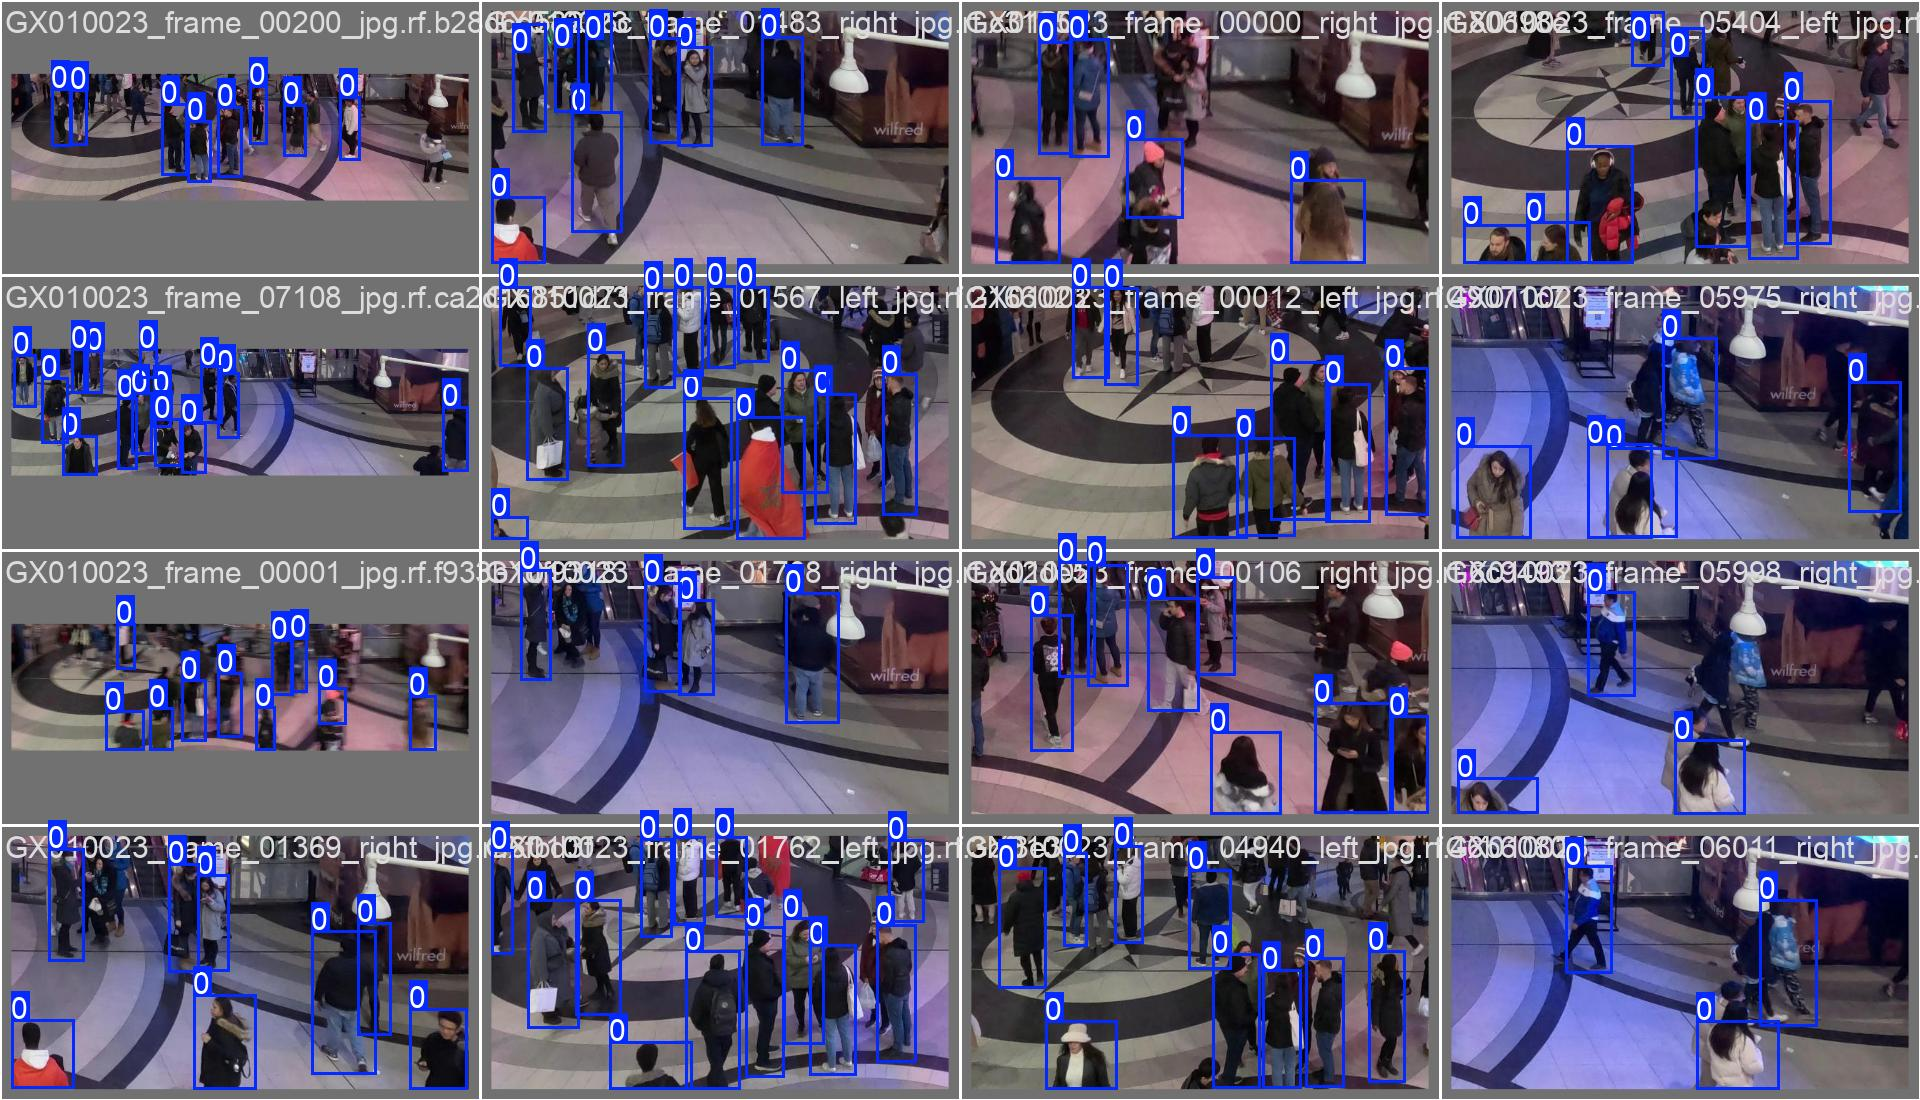
\includegraphics[width=1.00\textwidth]{./img/val_batch0_labels-yolov11s.jpg}
    \caption{Esempi di etichette su training}
    \label{fig:yolov11s-training-set}
\end{figure}

\subsubsection{Fase di validazione}
La fase di validazione dei modelli viene eseguita su un test set acquisito e annotato manualmente, in modo da poter visualizzare più concretamente le capacità dei modelli precedentemente addestrati. Di seguito è possibile visualizzare il codice di validazione per ciascun modello:

\begin{lstlisting}[language=Python, caption={Esempio di codice per la validazione dei modelli YOLO}, label={lst:val-yolo}]
from ultralytics import YOLO

model = YOLO("best-model-weights-to-evaluate.pt") 

results = model.val(data="/kaggle/input/test-set-for-ml-
project/test-set-for-ml-project/data.yaml", split = "test")

results.results_dict
\end{lstlisting}
È possibile sostituire il \texttt{best-model-weights-to-evaluate.pt} con i pesi migliori del modello di cui si vuole effettuare la validazione. Anche in questo caso viene fornito un file \texttt{.yaml} che permette di individuare il path corrispondente al test comprensivo di immagini e annotazioni. Il campo \texttt{.results\_dict} permette di visualizzare il dizionario delle metriche: precision, recall, mAP(50), mAP(50-95), fitness. I risultati verranno salvati dentro la cartella \texttt{run/detect/val[n]}.

%immagini da inserire%
\begin{figure}[H]
    \centering
    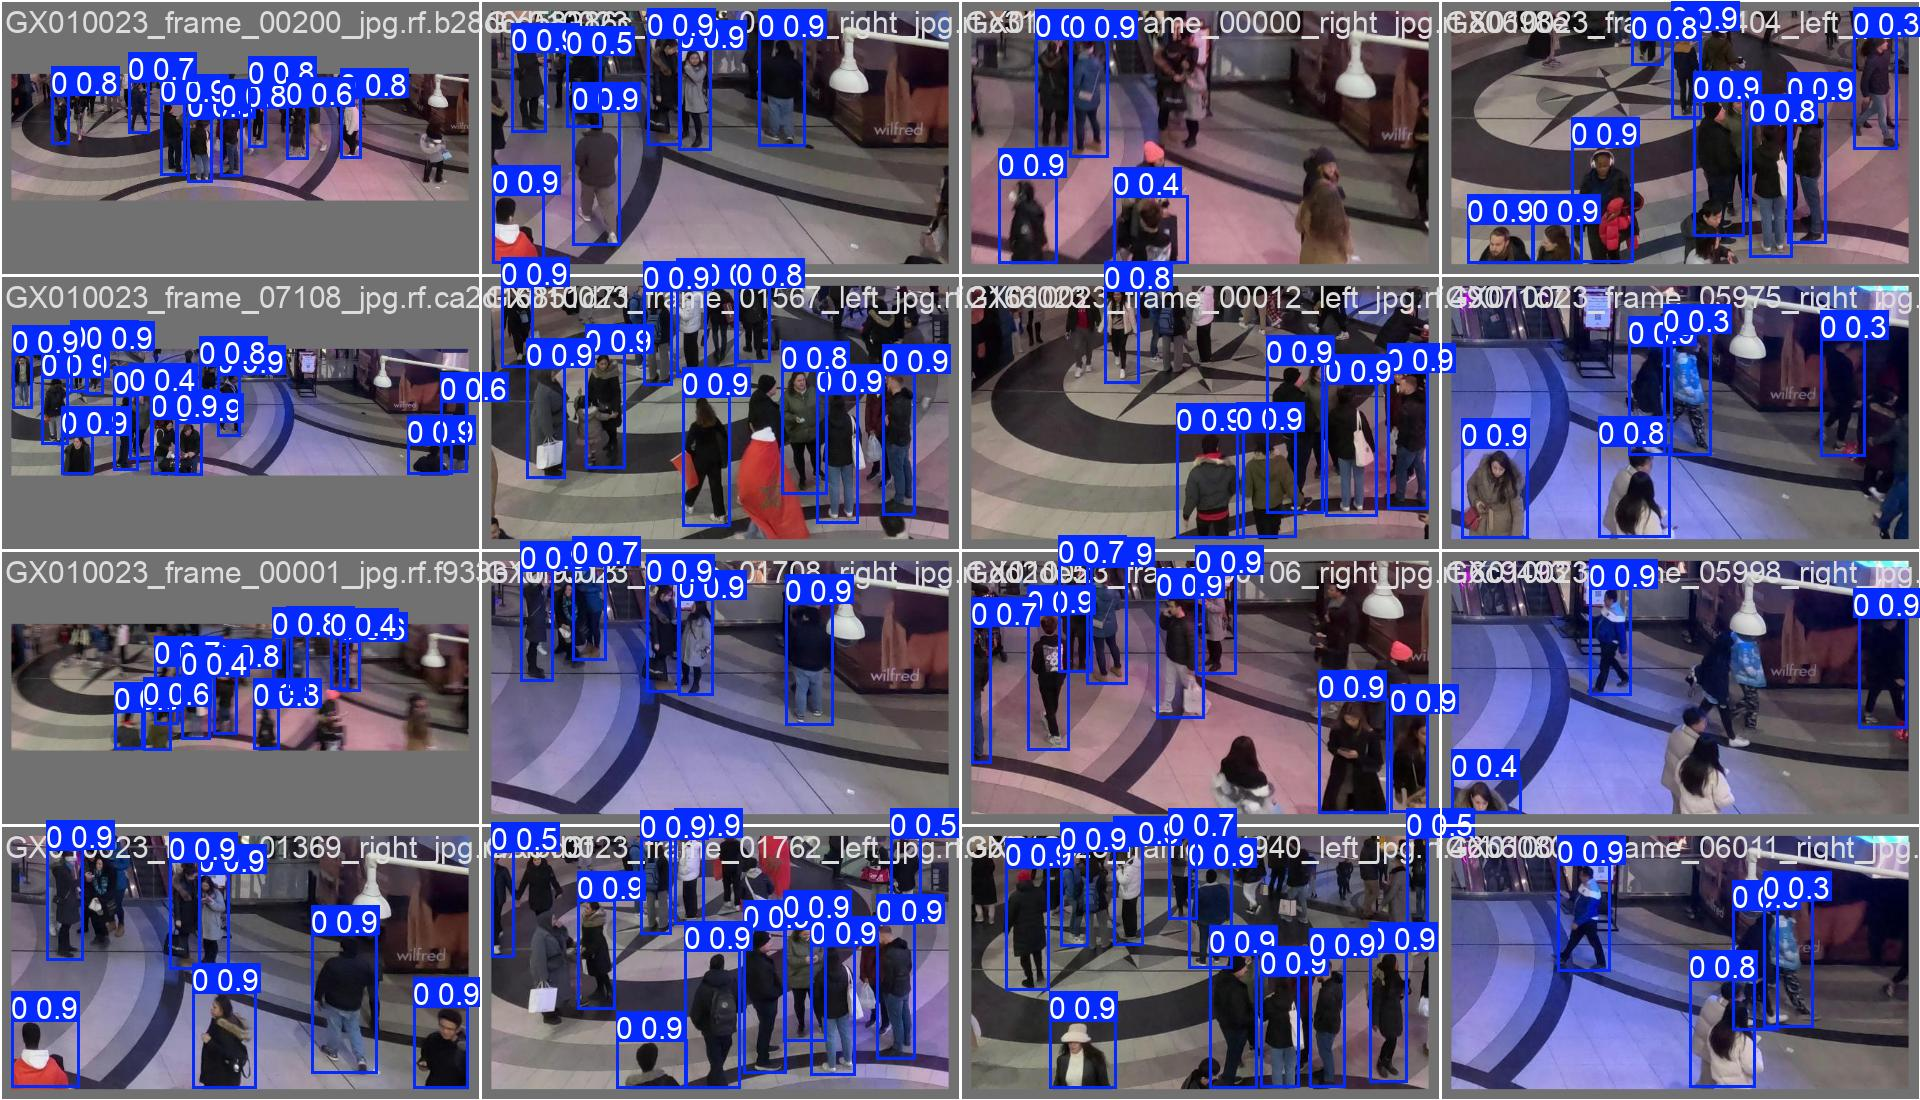
\includegraphics[width=1.00\textwidth]{./img/val_batch0_pred-yolov11s.jpg}
    \caption{Esempi di validazione su split = Validation Set con YOLOv11s}
    \label{fig:yolov11s-validation-set}
\end{figure}

\begin{figure}[H]
    \centering
    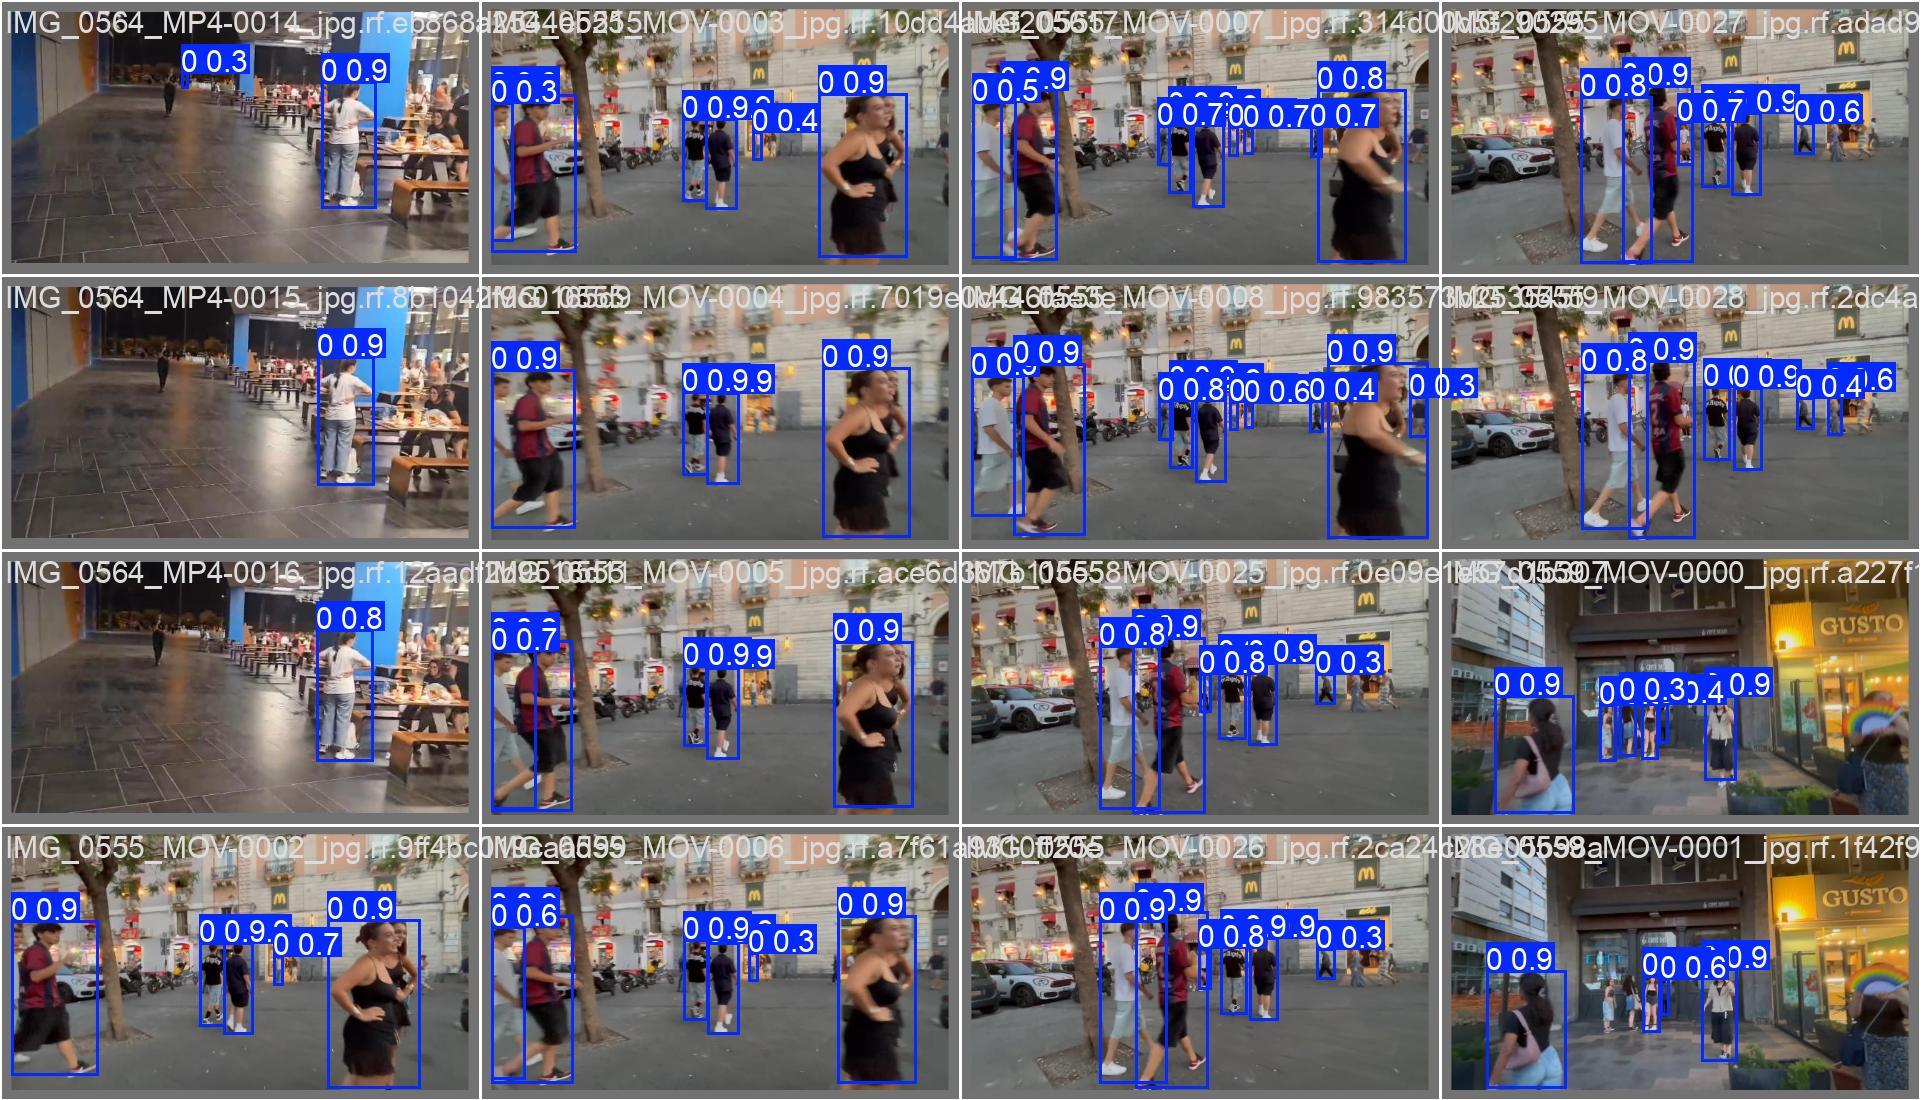
\includegraphics[width=1.00\textwidth]{./img/val_batch1_pred-yolov11s.jpg}
    \caption{Esempi di validazione su split = Test Set con YOLOv11s}
    \label{fig:yolov11s-test-set}
\end{figure}

\subsection{Faster R-CNN con Resnet50}
\subsubsection{Parametri di training}
Di seguito sono riportati i parametri principali adottati per l’addestramento del modello \textit{two-stage} \textbf{Faster RCNN} con backbone \textbf{Resnet50}, architettura con 50 layer convoluzionali. I valori scelti tengono conto della disponibilità computazionale data dalla piattaforma Kaggle (\textbf{GPU P100}).
\begin{table}[H]
\centering
\begin{tabular}{|l|c|p{5.2cm}|}
\hline
\textbf{Parametro} & \textbf{Valore utilizzato} & \textbf{Descrizione} \\
\hline
\texttt{epochs} & 30 & Numero di epoche (iterazioni complete sul dataset di train) \\
\hline
\texttt{patience} & \texttt{n/a} & Epoche di tolleranza per \textit{early stopping} in assenza di miglioramenti \\
\hline
\texttt{lr0} (Learning Rate iniziale) & 0.001 & Passo di apprendimento iniziale per l’ottimizzatore \\
\hline
\texttt{weight decay} & 0.0005 & Coefficiente di regolarizzazione L2 (\textit{Weight Decay}) \\
\hline
\texttt{momentum} & 0.9 & Consente di mantenere l'inerzia del movimento dei pesi
nel tempo \\
\hline
\texttt{gamma} & 0.1 & Controlla quanto peso hanno i singoli punti di addestramento nel determinare il \textit{decision boundary} \\
\hline
\texttt{step\_size} & 3 & Determina la dimensione dei passi fatti durante la discesa del gradiente \\
\hline
\texttt{imgsz} & 640$\times$640 & Dimensione di input delle immagini di training (in pixel) \\
\hline
\texttt{batch} & 4 & Dimensione del batch (numero di immagini per iterazione) \\
\hline
\texttt{ottimizzatore} & SDG & Algoritmo di ottimizzazione utilizzato (es. Adam, SGD, ecc.) \\
\hline
\end{tabular}
\caption{Parametri principali utilizzati per il training del modello}
\label{tab:parametri-training-faster-rcnn}
\end{table}

\subsubsection{Organizzazione della directory per il training}
I file necessari sono stati caricati nella directory \texttt{/kaggle/input/new-dataset-}\\
\texttt{for-ml-project-coco}, che contiene l'intero dataset annotato e i file di annotazione \texttt{\_annotations.coco.json}. La struttura della directory rispetta lo standard previsto dal modello Faster RCNN con suddivisione tra \textbf{train},\textbf{ valid }e \textbf{test}, ciascuno contenente le rispettive sottocartelle \textbf{images}. Al loro interno si trovano non solo i vari frame, ma anche i file di annotazione in formato \texttt{.json}, seguendo lo standard del dataset COCO. Di seguito viene mostrata la struttura completa:

\begin{verbatim}
/kaggle/input/new-dataset-for-ml-project-coco/
|-- train/
|   |-- images/
|       |-- _annotations.coco.json
|       |-- img.png
|-- val/
|   |-- images/
|       |-- _annotations.coco.json
|       |-- img.png
|-- test/
    |-- images/
        |-- _annotations.coco.json
        |-- img.png
\end{verbatim}
Le annotazioni in formato \texttt{COCO JSON} rappresentano uno standard ampiamente utilizzato nel campo dell'Object Detection. Forniscono un modo strutturato per memorizzare immagini includendo informazioni sugli oggetti, le loro bounding boxes, categorie e altri metadati. Tipicamente all'interno di un file di annotazione \texttt{COCO} è possibile trovare cinque campi principali: \texttt{info}, \texttt{licences}, \texttt{images}, \texttt{annotations}, \texttt{categories}. Viene sempre indicata una supercategoria consistente nel \textit{background} dell'immagine come nel caso dello studio e, ancora, una categoria a seguire: 1 (persona). \textit{Si noti invece che nel caso di YOLO, la categoria persona viene codificata con 0}.

\subsubsection{Fase di training}
La fase di training del modello è stata eseguita in ambiente \textit{Kaggle}, sfruttando GPU P100 per una runtime totale di 2h 54m.\\
Il codice di addestramento per il modello è il seguente:
\begin{lstlisting}[language=Python, caption={Esempio di codice per il training del modello Resnet}, label={lst:train-resnet}]
model.train()
total_loss = 0
num_batches = len(data_loader)
    
progress_bar = tqdm(data_loader, desc=f"Training-
Epoch{epoch+1}")
    
for batch_idx, (images, targets) in enumerate(progress_bar):
    # Move data to device
    images = [img.to(device) for img in images]
    targets = [{k: v.to(device) for k, v in t.items()} 
    for t in targets]
        
    # Forward pass
    loss_dict = model(images, targets)
    losses = sum(loss for loss in loss_dict.values())
        
    # Backward pass
    optimizer.zero_grad()
    losses.backward()
    optimizer.step()
        
    total_loss += losses.item()
        
    # Update progress bar
    progress_bar.set_postfix({
        'Loss': f'{losses.item():.4f}',
        'AvgLoss': f'{total_loss/(batch_idx+1):.4f}'
    })
    
return total_loss / num_batches
\end{lstlisting}
Durante la fase di allenamento è possibile visualizzare lo status del training mediante il widget della progress bar. Inoltre, per ogni epoca verrà stampata a video la misura di Train Loss, Val Loss, Epoca corrente e infine Learning Rate per l'epoca in questione.

\subsubsection{Fase di validazione}
La fase di validazione del modello è  eseguita su un test set acquisito e annotato manualmente, in modo da poter visualizzare e mettere a confronto con le capacità dei modelli YOLO precedentemente valutati. Di seguito è possibile visualizzare il codice di validazione per il modello:

\begin{lstlisting}[language=Python, caption={Esempio di codice per la validazione del modello Resnet}, label={lst:valid-resnet}]
def evaluate_model(model, data_loader, device, 
confidence_threshold = 0.5):
    # Evaluate the model on a dataset
    model.eval()
    
    all_predictions = []
    all_targets = []
    
    with torch.no_grad():
        for images, targets in tqdm(data_loader, desc="Evaluating"):
            images = [img.to(device) for img in images]
            
            predictions = model(images)
            
            # Process predictions and targets
            for pred, target in zip(predictions, targets):
                scores = pred['scores']
                keep = scores >= confidence_threshold
                
                pred_filtered = {
                    'boxes': pred['boxes'][keep].cpu().numpy(),
                    'scores': pred['scores'][keep].cpu().numpy(),
                    'labels': pred['labels'][keep].cpu().numpy()
                }
                
                target_processed = {
                    'boxes': target['boxes'].cpu().numpy(),
                    'labels': target['labels'].cpu().numpy()
                }
                
                all_predictions.append(pred_filtered)
                all_targets.append(target_processed)
    
    return all_predictions, all_targets


def calculate_iou(box1, box2):
    # Calculate intersection coordinates
    x1 = max(box1[0], box2[0])
    y1 = max(box1[1], box2[1])
    x2 = min(box1[2], box2[2])
    y2 = min(box1[3], box2[3])
    
    # Calculate intersection area
    if x2 <= x1 or y2 <= y1:
        return 0.0
    
    intersection = (x2 - x1) * (y2 - y1)
    
    # Calculate union area
    area1 = (box1[2] - box1[0]) * (box1[3] - box1[1])
    area2 = (box2[2] - box2[0]) * (box2[3] - box2[1])
    union = area1 + area2 - intersection
    
    return intersection / union if union > 0 else 0.0


def calculate_metrics(predictions, targets, iou_threshold = 0.5):
    # Calculate detection metrics
    
    all_pred_boxes = []
    all_pred_scores = []
    all_gt_boxes = []
    
    # Collect all predictions and ground truths
    for pred, target in zip(predictions, targets):
        all_pred_boxes.extend(pred['boxes'])
        all_pred_scores.extend(pred['scores'])
        all_gt_boxes.extend(target['boxes'])
    
    # Sort predictions by confidence score
    sorted_indices = np.argsort(all_pred_scores)[::-1]
    sorted_pred_boxes = [all_pred_boxes[i] for i in sorted_indices]
    
    # Calculate matches
    tp = 0  # True positives
    fp = 0  # False positives
    matched_gt = set()  # Keep track of matched ground truth boxes
    
    for pred_box in sorted_pred_boxes:
        best_iou = 0.0
        best_gt_idx = -1
        
        for gt_idx, gt_box in enumerate(all_gt_boxes):
            if gt_idx in matched_gt:
                continue
            
            iou = calculate_iou(pred_box, gt_box)
            if iou > best_iou:
                best_iou = iou
                best_gt_idx = gt_idx
        
        if best_iou >= iou_threshold:
            tp += 1
            matched_gt.add(best_gt_idx)
        else:
            fp += 1
    
    fn = len(all_gt_boxes) - tp  # False negatives

    precision = tp / (tp + fp) if (tp + fp) > 0 else 0.0
    recall = tp / (tp + fn) if (tp + fn) > 0 else 0.0
    f1_score = 2 * (precision * recall) / (precision + recall) 
    if (precision + recall) > 0 else 0.0
    
    return {
        'precision': precision,
        'recall': recall,
        'f1_score': f1_score,
        'true_positives': tp,
        'false_positives': fp,
        'false_negatives': fn,
        'total_predictions': len(all_pred_boxes),
        'total_ground_truth': len(all_gt_boxes)
    }
\end{lstlisting}
I risultati di validazione del modello permettono di concentrarsi su \textit{precision}, \textit{recall}, la \textit{F1 score}, i \textit{True Positives}, \textit{False Positives}, \textit{False Negatives}, \textit{Total Predictions}, \textit{Total Ground Truth}. A differenza dei modelli YOLO, non verranno generati dei grafici. Tuttavia è possibile effettuare e visualizzare le detection di frame e video mediante gli appositi metodi definiti.

\subsection{Demo e funzionamento}
La presente sezione è interamente dedicata alla demo implementata per poter testare i modelli su nuovi dati. La demo è stata scritta interamente in Python, appoggiandosi sulla piattaforma \textit{Kaggle} per poter usufruire liberamente delle risorse computazionali senza necessità di installare librerie nel proprio ambiente. È pronta all'uso, basterà cliccare su \texttt{Copy \& Edit} per poter modificare le celle del notebook. Presenta le seguenti funzionalità:
\begin{itemize}
    \item Caricamento di un'immagine o di un video su cui effettuare la predizione tramite tasto di \texttt{Upload}
    \item Scelta del modello con cui effettuare la predizione. Sarà possibile caricare il dataset con i migliori pesi reso pubblico. Si potrà selezionare dunque tra YOLOv8m, YOLOv10n, YOLOv11s, Resnet50.
    \item Visualizzazione grafica dei risultati: una volta terminato il processo di predizione sarà possibile visualizzare nella cartella \texttt{working} di \textit{Kaggle} il risultato in formato \texttt{.png} e in formato \texttt{.avi|.mp4} per i video.
    \item Conteggio delle persone presenti per un'immagine, e una media di persone presenti per un video fornito in input.
\end{itemize}
Per poter utilizzare la demo basterà avviare la sessione prestando attenzione a modificare il path relativo al dataset contenente una o più immagini, oppure contenente uno o più video, o entrambi. 
\begin{lstlisting}[language=Python, caption={Path relativo al dataset}, label={lst:path-demo}]
import torch

device = torch.device('cuda' if torch.cuda.is_available() 
else 'cpu')
 
INPUT_FILE_PATH = "/kaggle/input/test-video-set/IMG_0555.MP4"
WORKING_PATH = "/kaggle/working/"
\end{lstlisting}
In questo modo sarà, dunque, possibile procedere alla fase successiva in cui celle differenti del \textit{notebook} potranno essere eseguite al fine di produrre il risultato desiderato. Nel caso dell'esempio sopra riportato la modalità è di video prediction dunque si avrà:\\
\begin{lstlisting}[language=Python, caption={Esempio di video predict su YOLOv8m}, label={lst:video-demo}]
model = YOLO("/kaggle/input/best-weights-for-model/best 
yolov8m.pt")
results = model.predict(source = INPUT_FILE_PATH, save = 
True, project = 'runs/detect', name = 'exp')"
\end{lstlisting}
È possibile importare il dataset \texttt{best-weights-for-model} con i migliori pesi per i modelli allenati nello studio tramite il seguente link: \href{https://www.kaggle.com/datasets/denisecilia/best-weights-for-model}{Best Weights Dataset}\\
È possibile visualizzare un breve video tutorial sulla demo mediante questo link: \href{https://drive.google.com/file/d/1NDn_j8GwivCiABEhohK7GARY8-FcGkur/view?usp=drive_link}{Demo}\\
\textbf{Nota:} Si tratta di una demo su nuovi dati. Non è necessario caricare le bounding box relative a ciascun file poiché non verrà calcolata alcuna metrica. È una visualizzazione delle potenzialità dei modelli addestrati in questo studio. \\
Si consiglia inoltre di effettuare il pre-processing dei dati con una resize delle immagini o dei video alle dimensioni \textbf{640x640} utilizzate nello studio.
Il link è seguente: \href{https://www.kaggle.com/code/denisecilia/demo-for-machine-learning-project?scriptVersionId=249249609}{Demo notebook}

\begin{figure}[H]
    \centering
    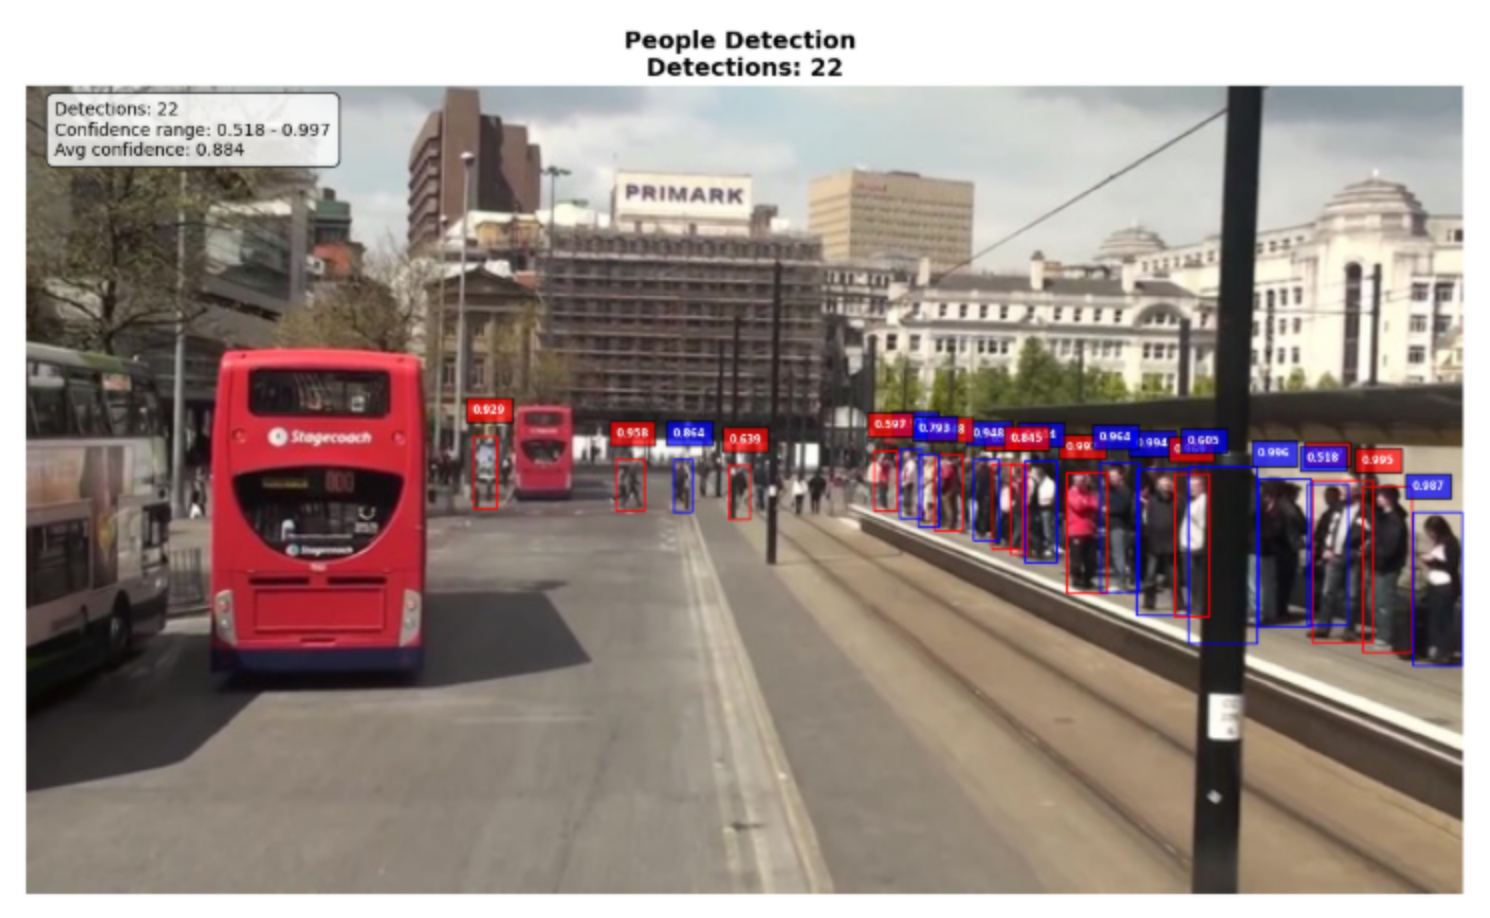
\includegraphics[width=1.00\textwidth]{./img/output-demo-example.png}
    \caption{Esempio di output della Demo su Prediction Frame di Faster R-CNN}
    \label{fig:demo-output}
\end{figure}

\section{Risultati}
Questo capitolo è dedicato all'analisi dei risultati conseguiti grazie alle fasi di training e validazione dei modelli di Object Detection impiegati nello studio. \\
Il training è stato effettuato utilizzando il dataset denominato "nome del dataset", con l'ausilio di una \textbf{GPU P100} attraverso l'ambiente di sviluppo offerto dalla piattaforma \textit{Kaggle}.\\
Nelle sezioni successive, verranno presentati in dettaglio grafici e tabelle che riassumono le principali misure di valutazione calcolate sui diversi modelli.\\

\subsection{Performance dei modelli YOLO}
Di seguito, viene presentata una tabella riassuntiva delle performance ottenute dai modelli della famiglia YOLO sul test set acquisito.

\begin{table}[h!]
\centering
\label{tab:yolo_pr_performance}
\begin{tabular}{|l|c|c|}
\hline
\textbf{Modello} & \textbf{Precision (B)} & \textbf{Recall (B)} \\
\hline
YOLOv10n         & 0.8437                 & 0.4830              \\
YOLOv11s         & 0.8035                 & 0.5594              \\
YOLOv8m          & 0.8965                 & 0.5368              \\
\hline
\end{tabular}
\caption{Performance dei modelli YOLO sul Test Set (Precisione e Recall)}
\end{table}

\begin{table}[h!]
\centering
\label{tab:yolo_map_performance}
\begin{tabular}{|l|c|c|c|}
\hline
\textbf{Modello} & \textbf{mAP50 (B)} & \textbf{mAP50-95 (B)} & \textbf{Fitness} \\
\hline
YOLOv10n         & 0.5871             & 0.2981                & 0.3270           \\
YOLOv11s         & 0.6463             & 0.3333                & 0.3646           \\
YOLOv8m          & 0.6555             & 0.3276                & 0.3604           \\
\hline
\end{tabular}
\caption{Performance dei modelli YOLO sul Test Set (mAP e Fitness)}
\end{table}

\subsubsection{Grafici dei risultati sul test set}
\begin{figure}[H]
    \centering
    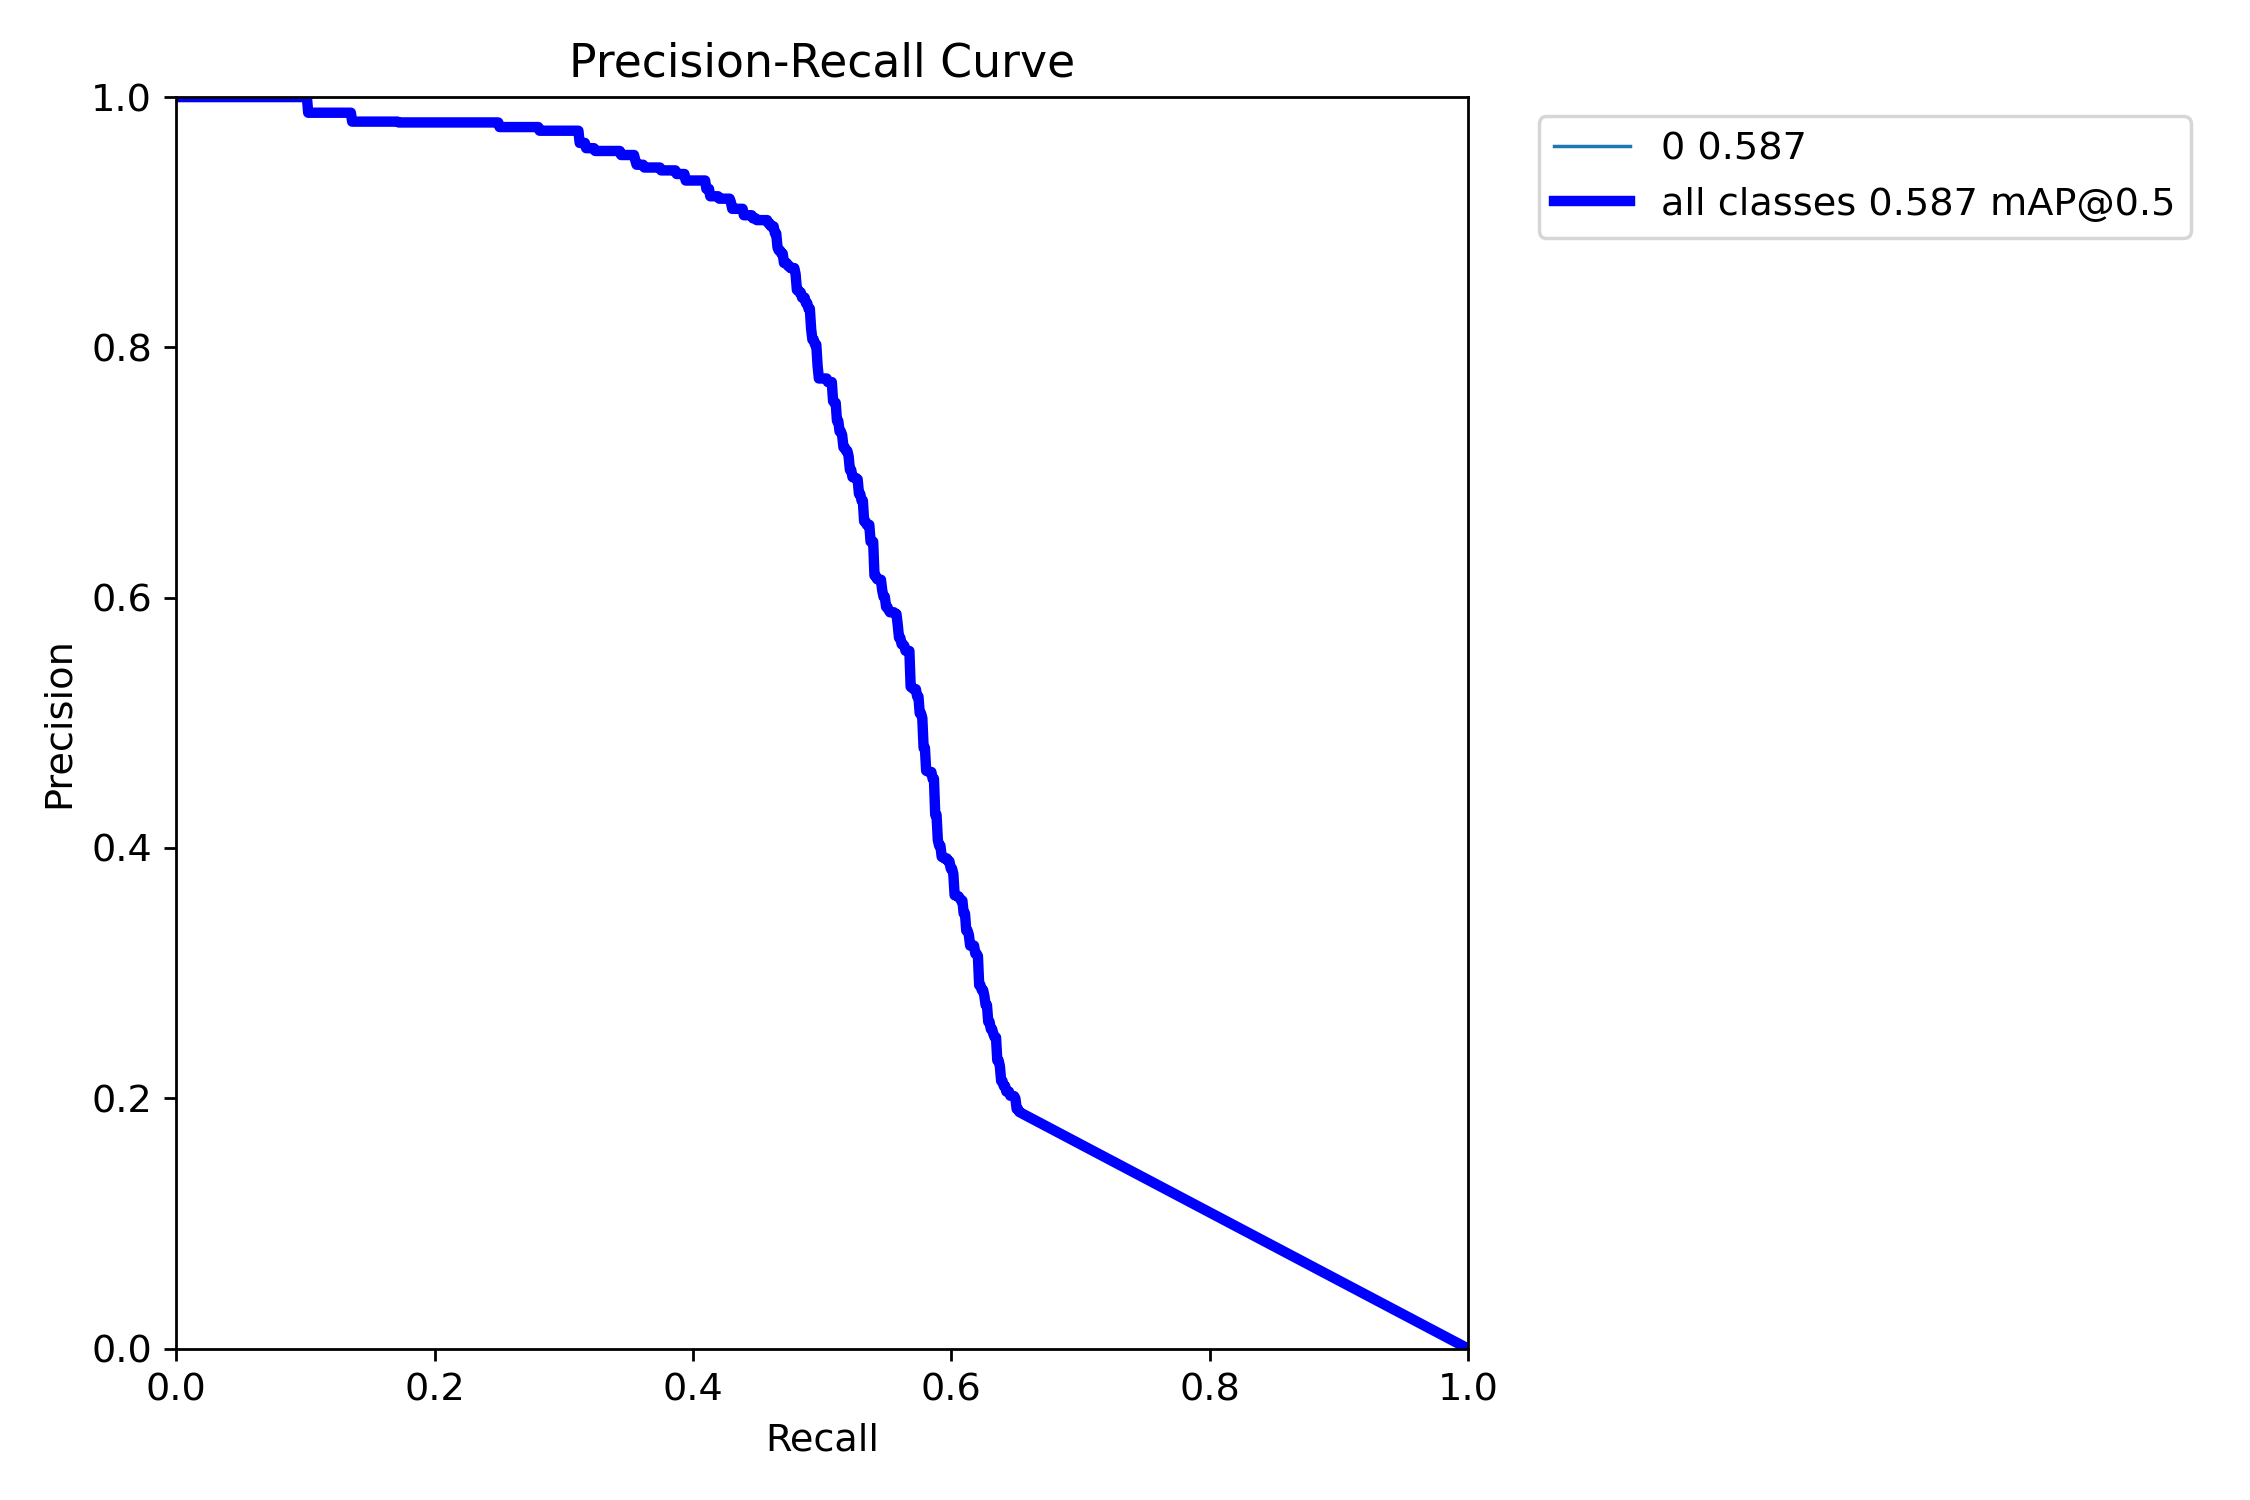
\includegraphics[width=0.8\textwidth]{./img/PR_curve-yolov8m.png}
    \caption{Curva di Precision-Recall per YOLOv8m}
    \label{fig:yolov8m-pr-curve}
\end{figure}

\begin{figure}[H]
    \centering
    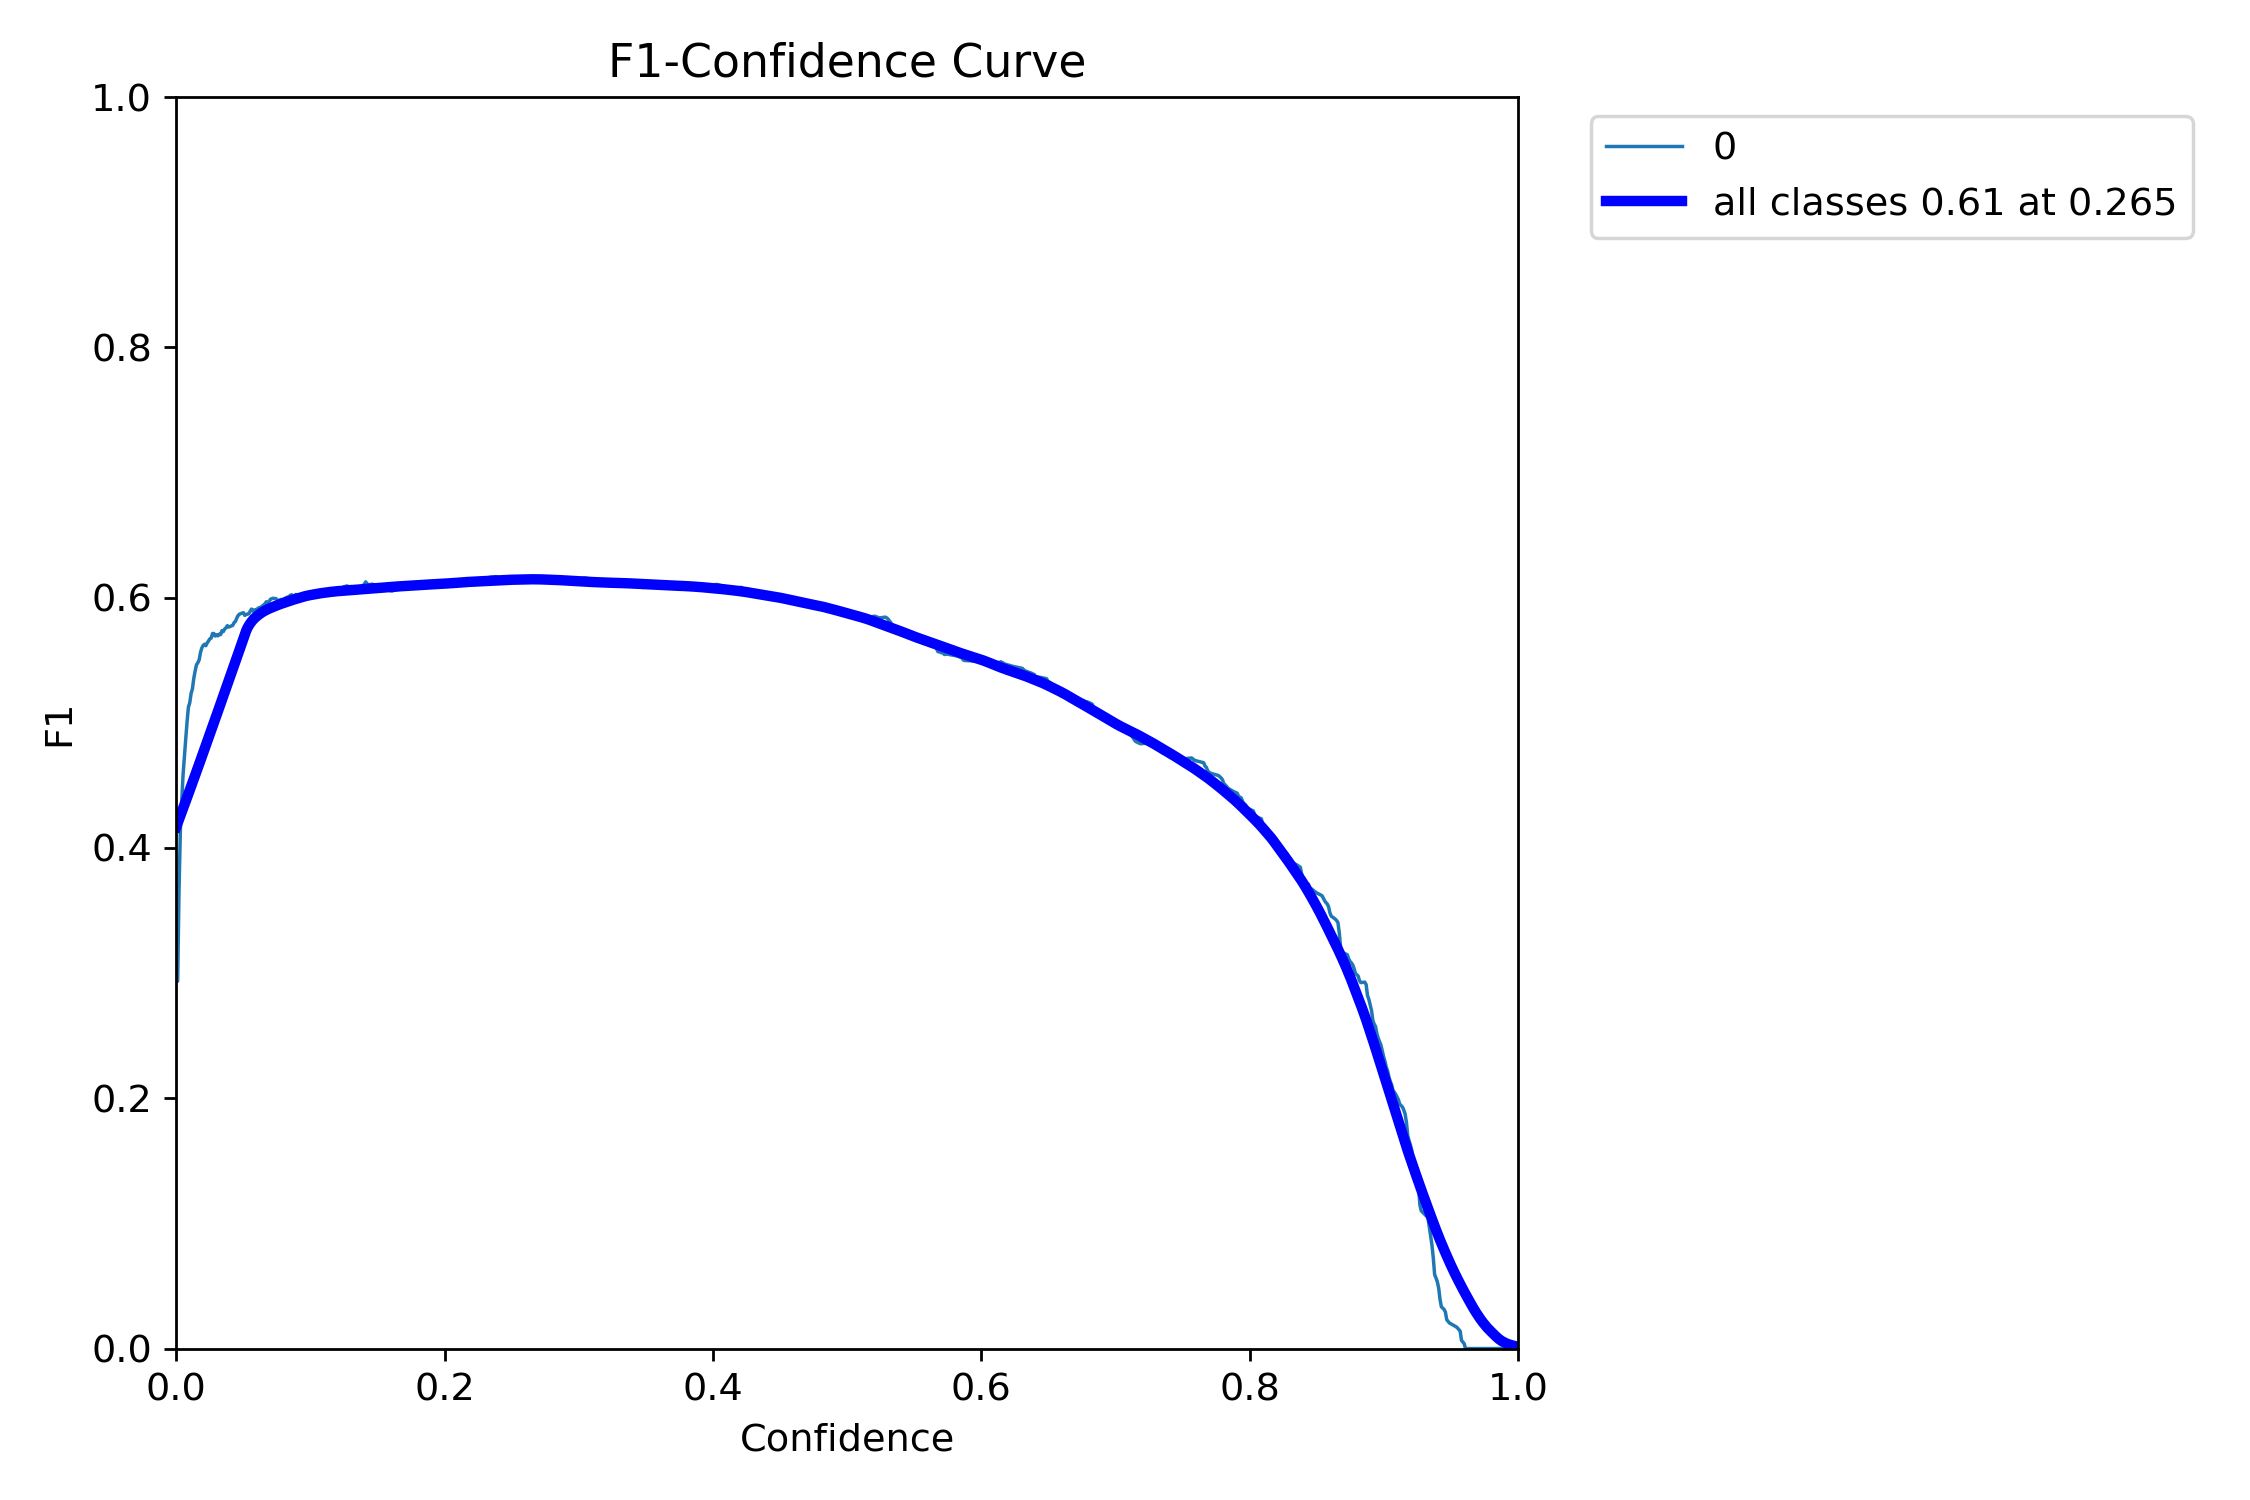
\includegraphics[width=0.9\textwidth]{./img/F1_curve-yolov8m.png}
    \caption{F1-Score per YOLOv8m}
    \label{fig:yolov8m-f1-score}
\end{figure}

\begin{figure}[H]
    \centering
    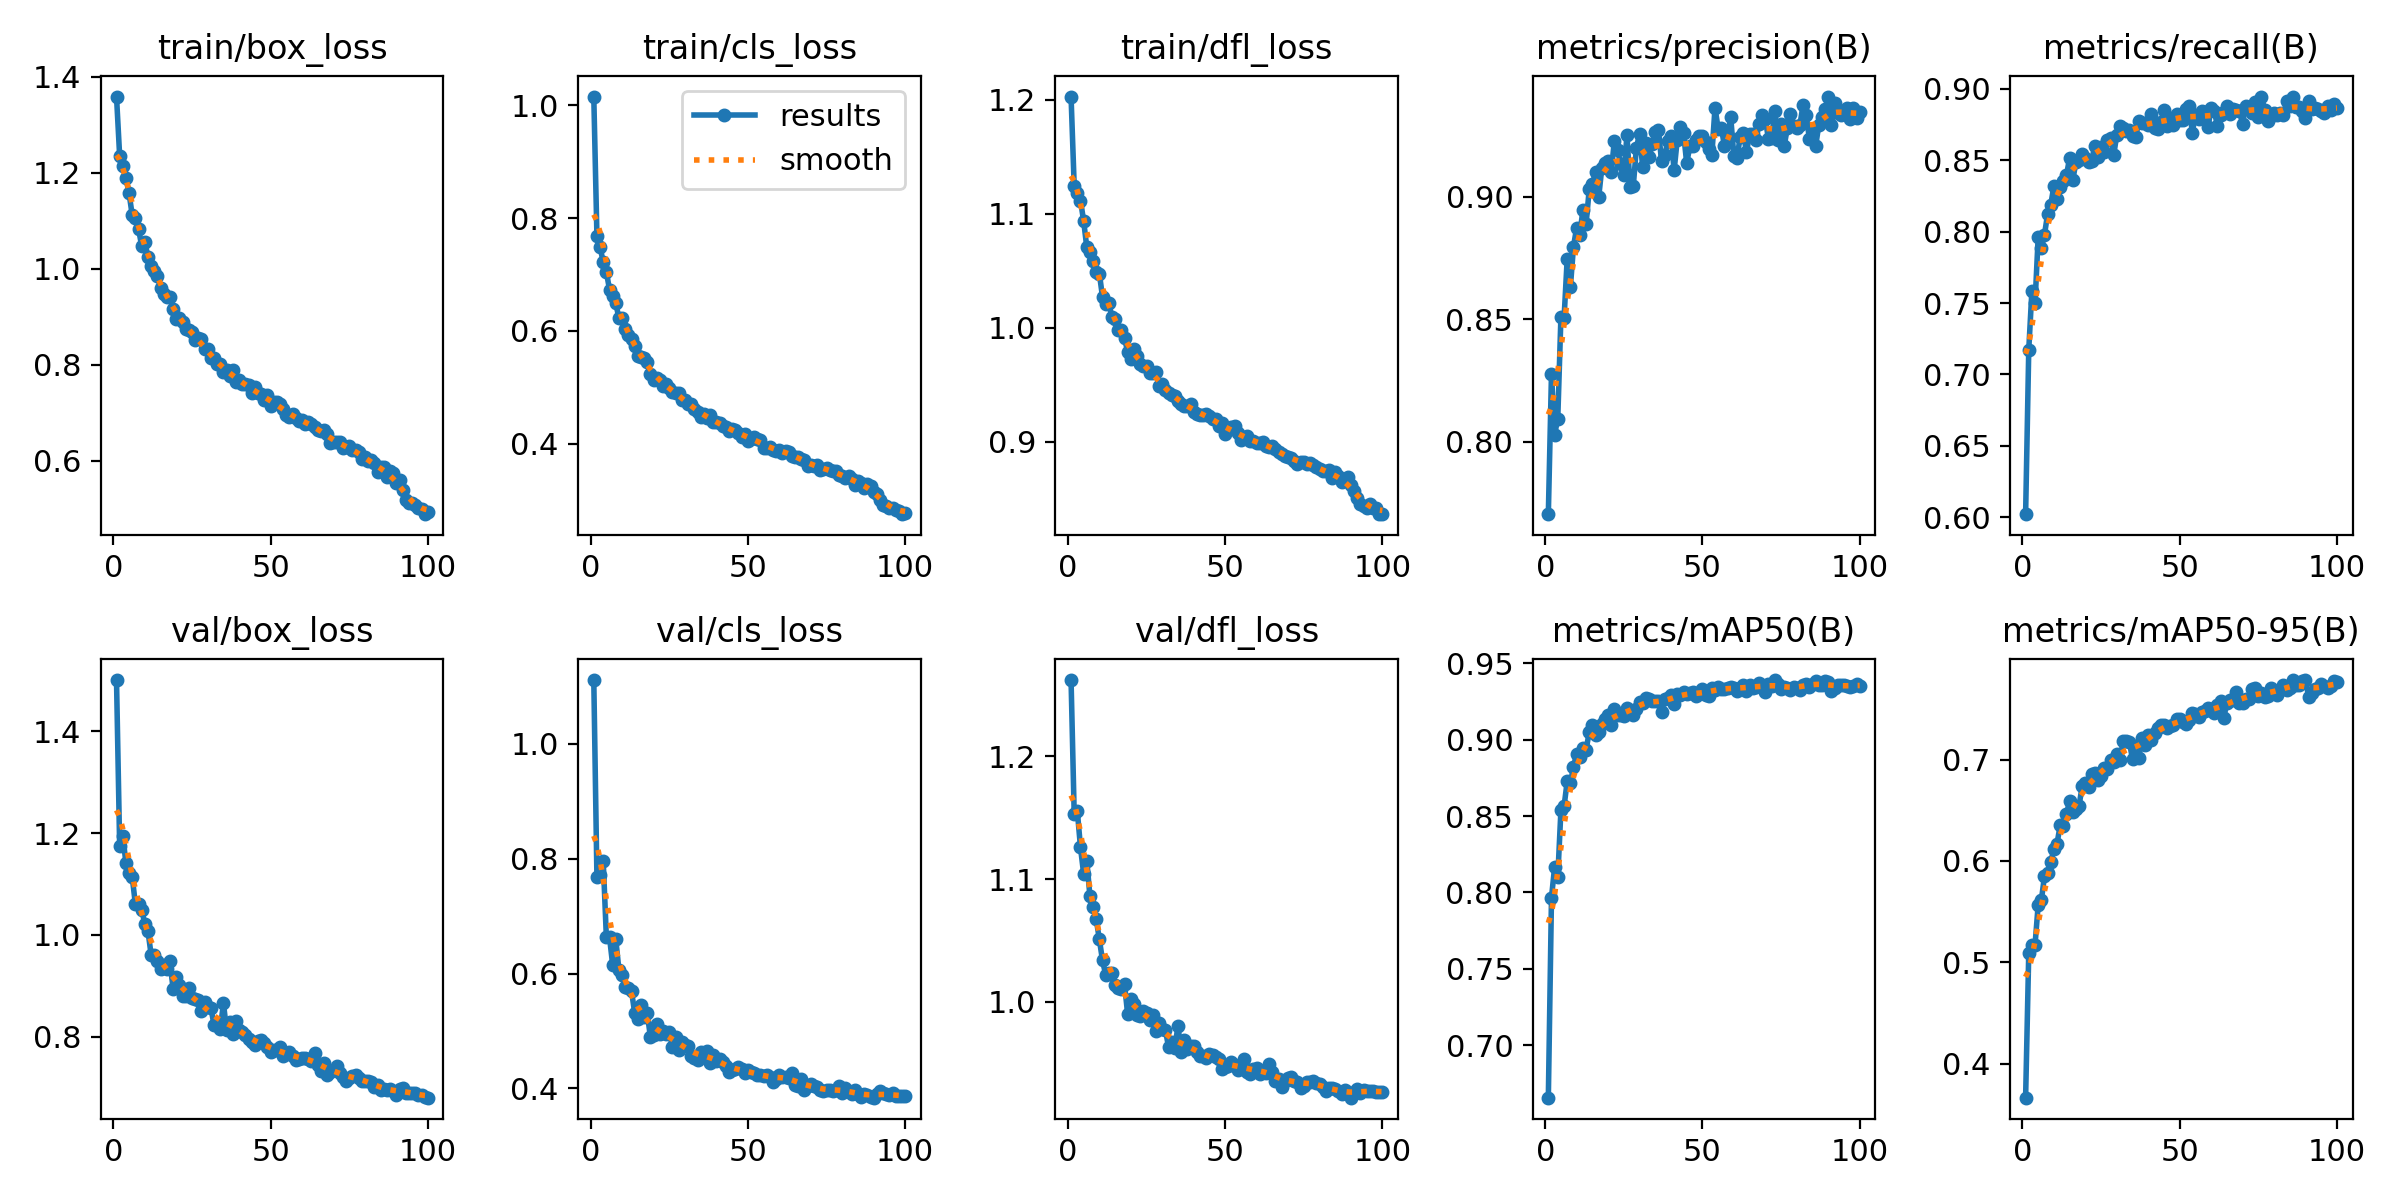
\includegraphics[width=1.1\textwidth]{./img/results-yolov8m.png}
    \caption{Risultati completi per YOLOv8m}
    \label{fig:yolov8m-results}
\end{figure}
%%%%%%%%%%%%%%%%%%%%%%%%%%%%%%%%%%%
\begin{figure}[H]
    \centering
    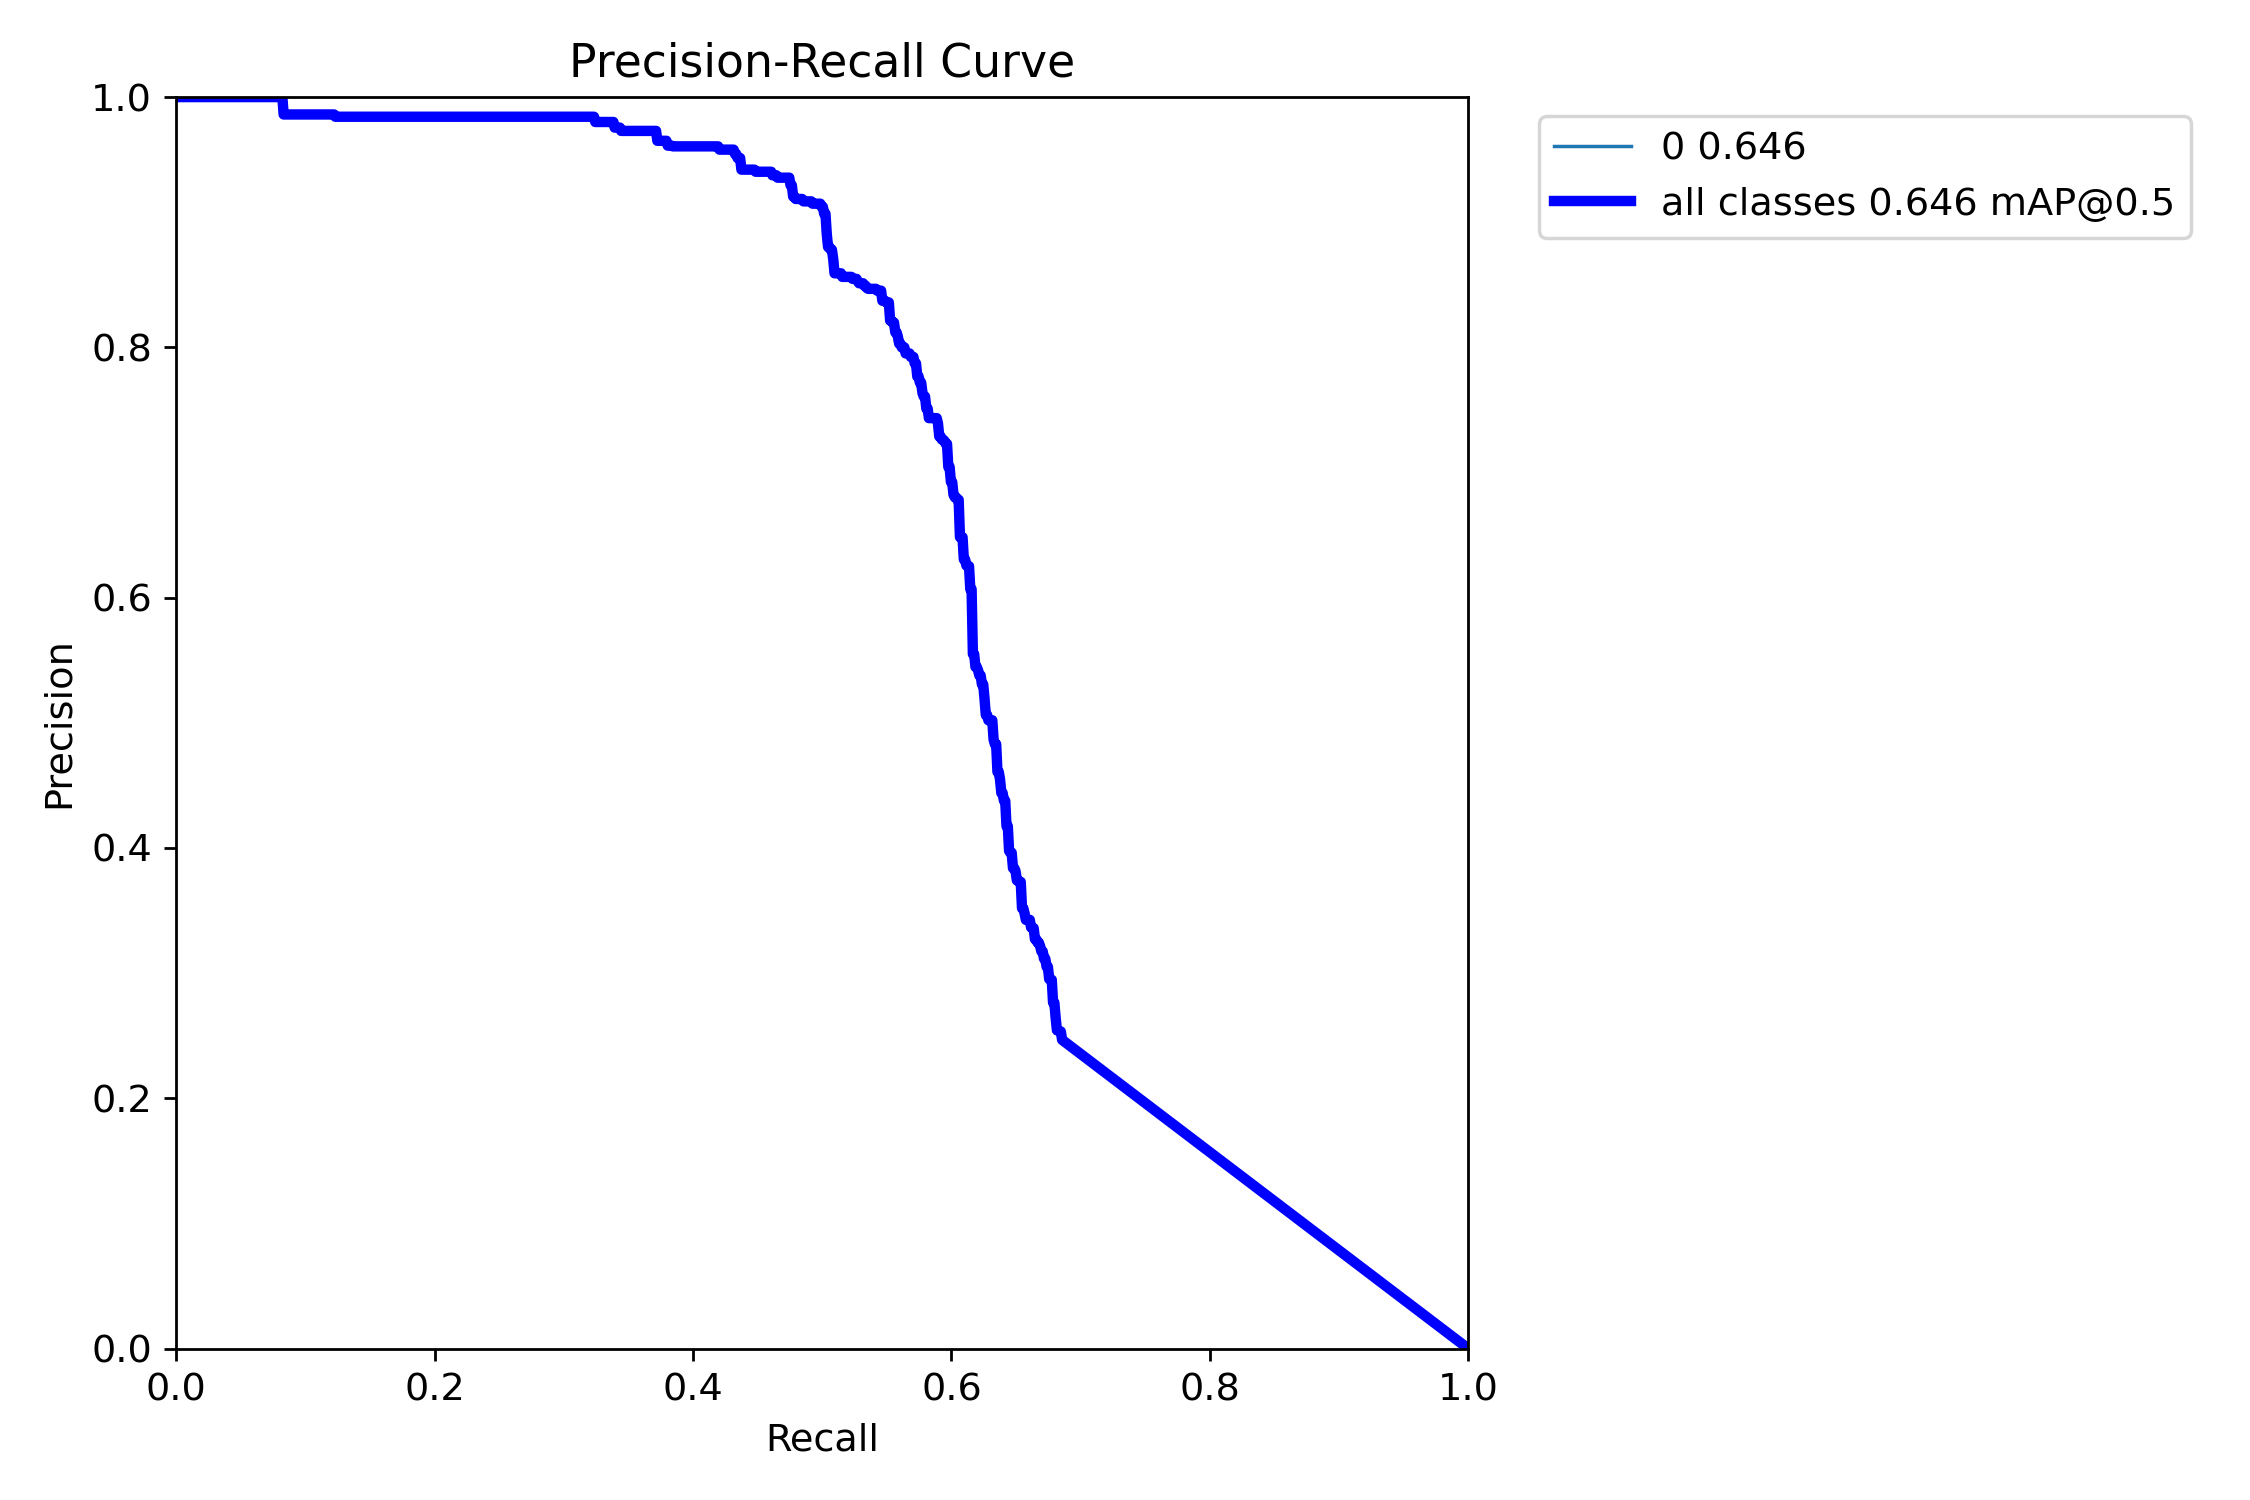
\includegraphics[width=0.9\textwidth]{./img/PR_curve-yolov10n.png}
    \caption{Curva di Precision-Recall per YOLOv10n}
    \label{fig:yolov10n-pr-curve}
\end{figure}

\begin{figure}[H]
    \centering
    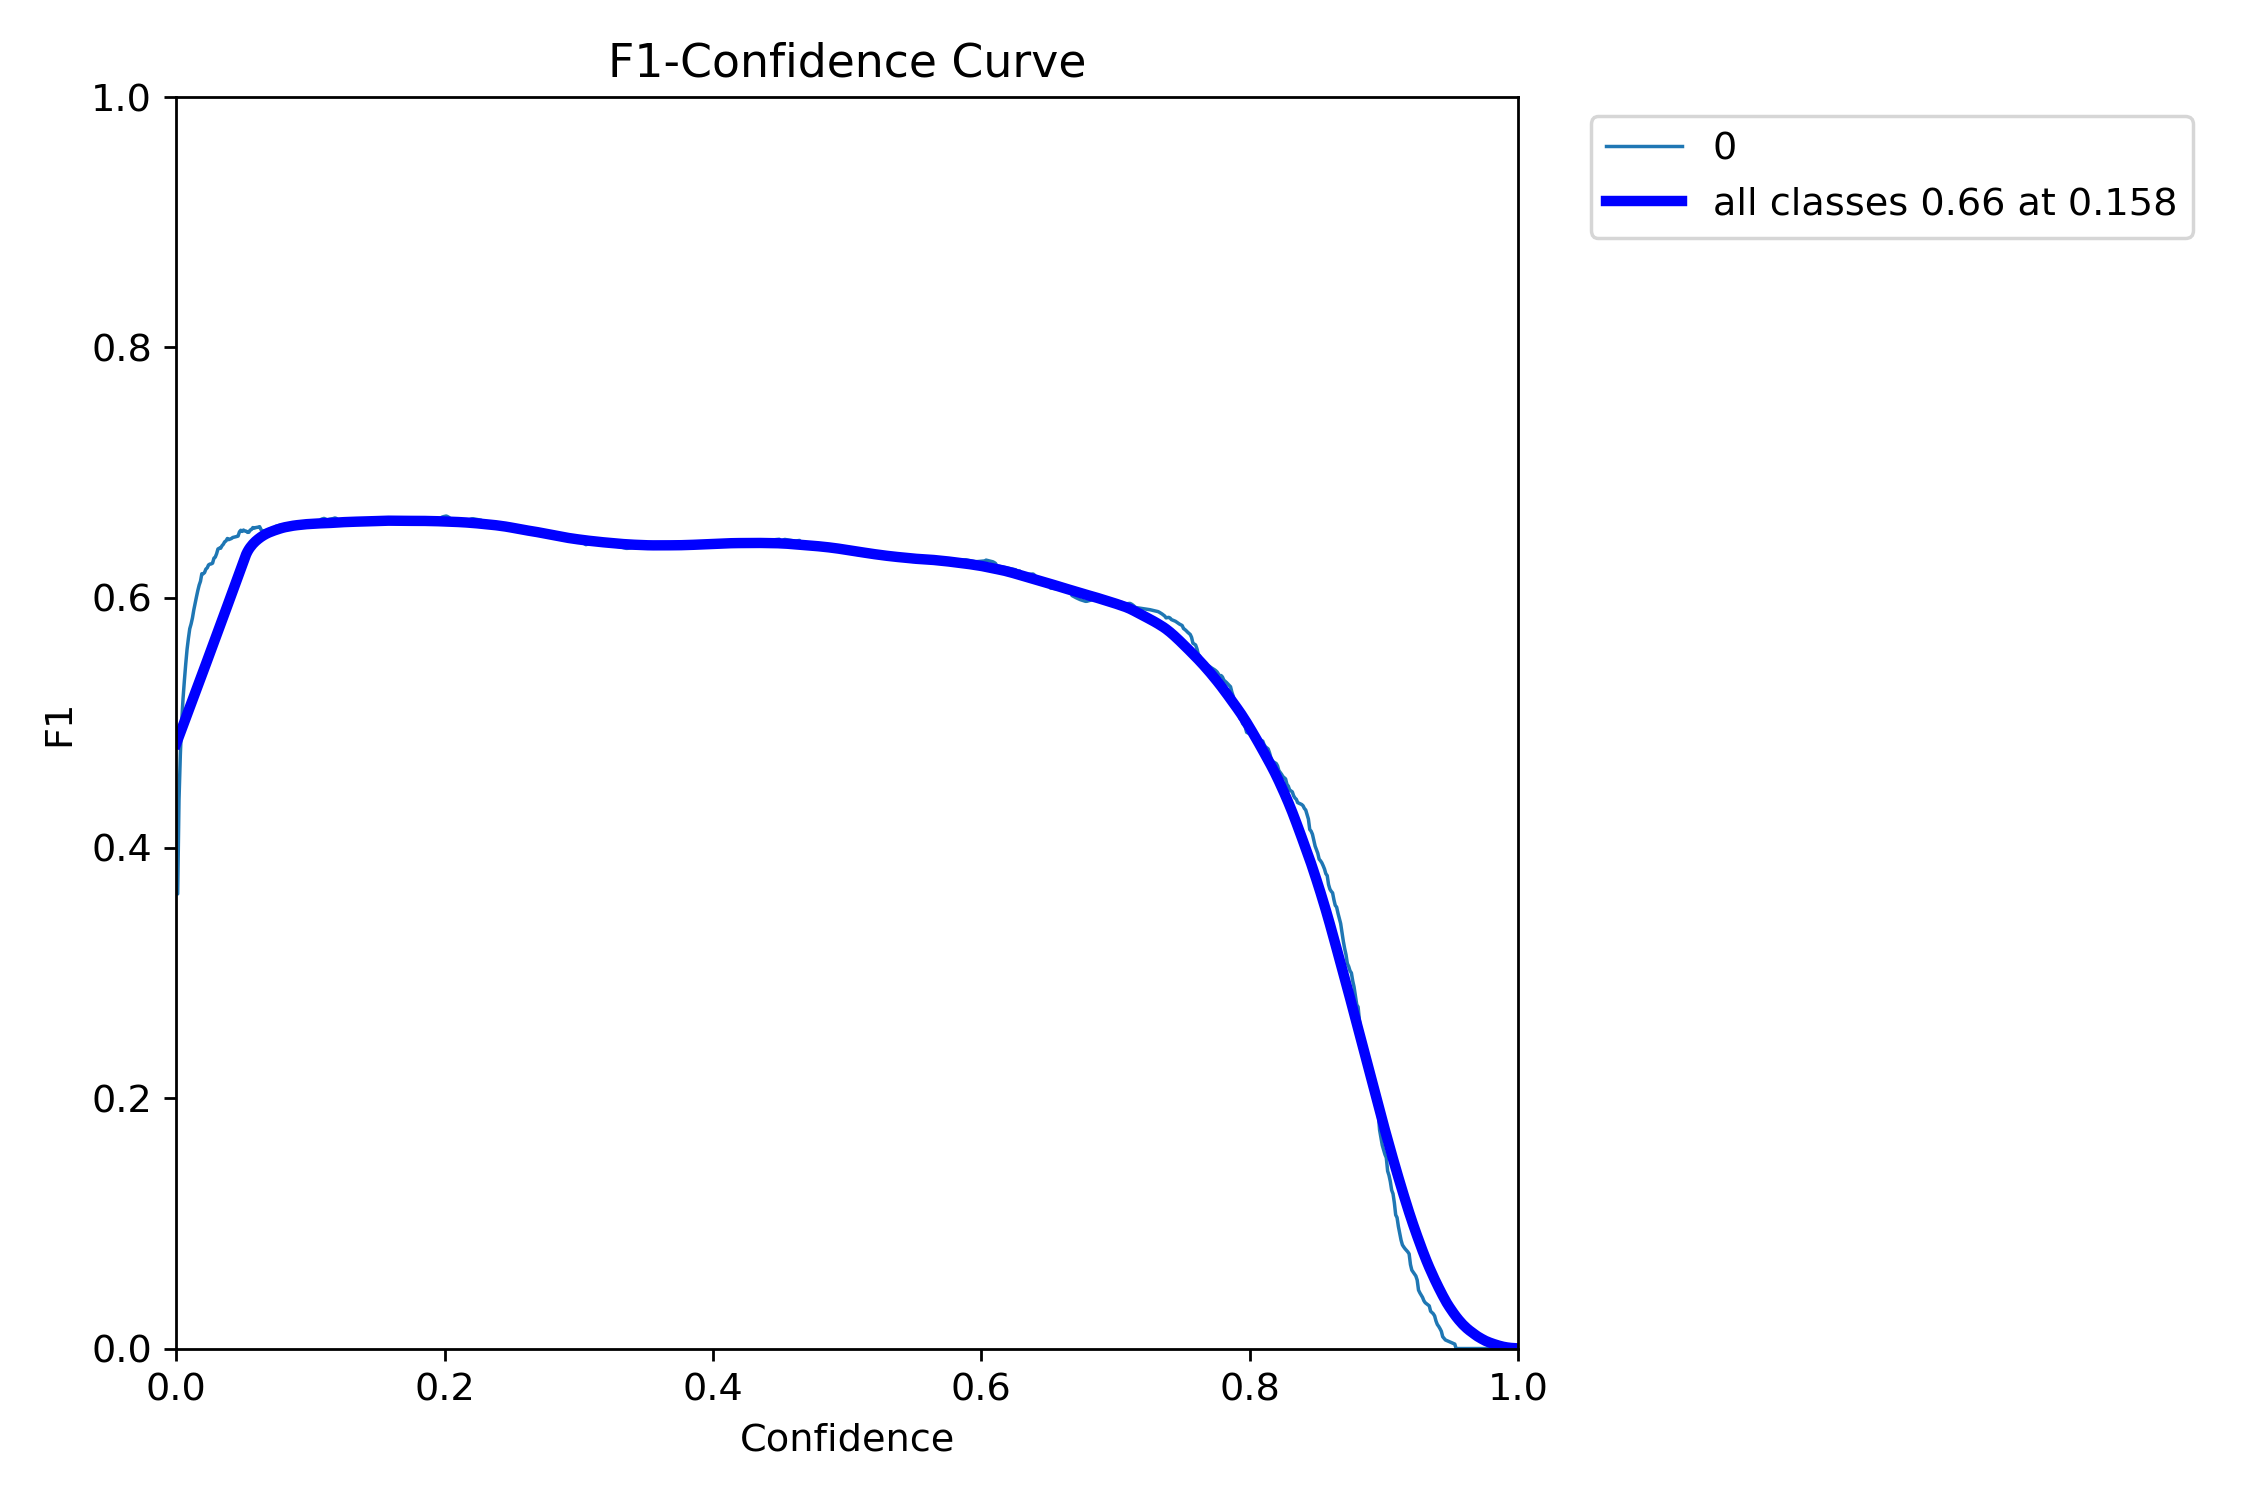
\includegraphics[width=0.9\textwidth]{./img/F1_curve-yolov10n.png}
    \caption{F1-Score per YOLOv10n}
    \label{fig:yolov10n-f1-score}
\end{figure}

\begin{figure}[H]
    \centering
    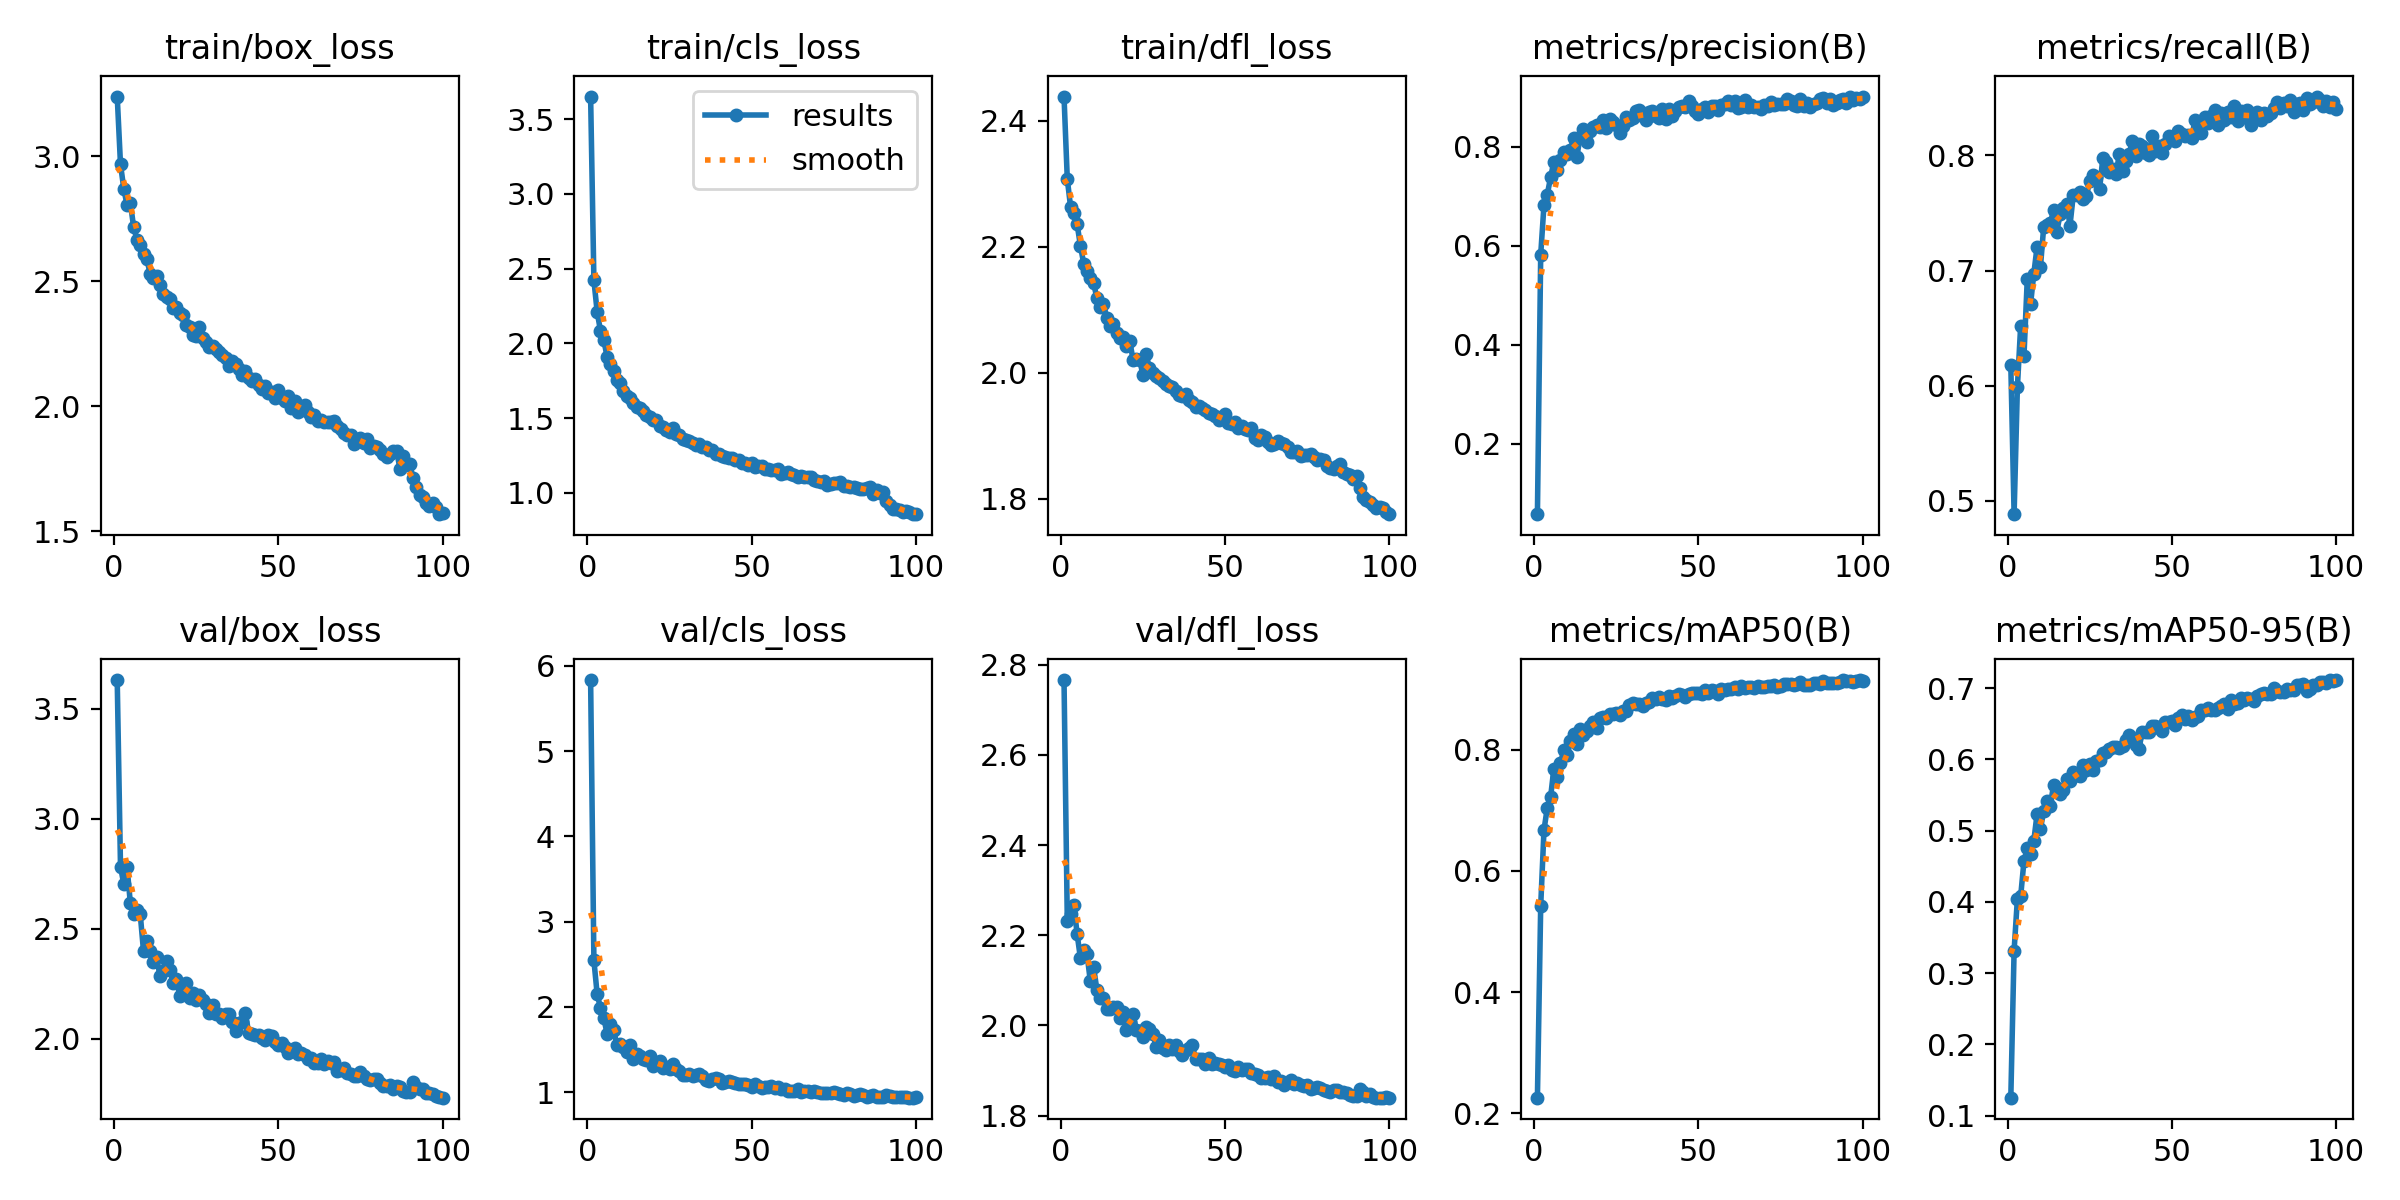
\includegraphics[width=1.1\textwidth]{./img/results-yolov10n.png}
    \caption{Risultati completi per YOLOv10n}
    \label{fig:yolov10n-results}
\end{figure}
%%%%%%%%%%%%%%%%%%%%%%%%%%%%%%%%%
\newpage
\begin{figure}[H]
    \centering
    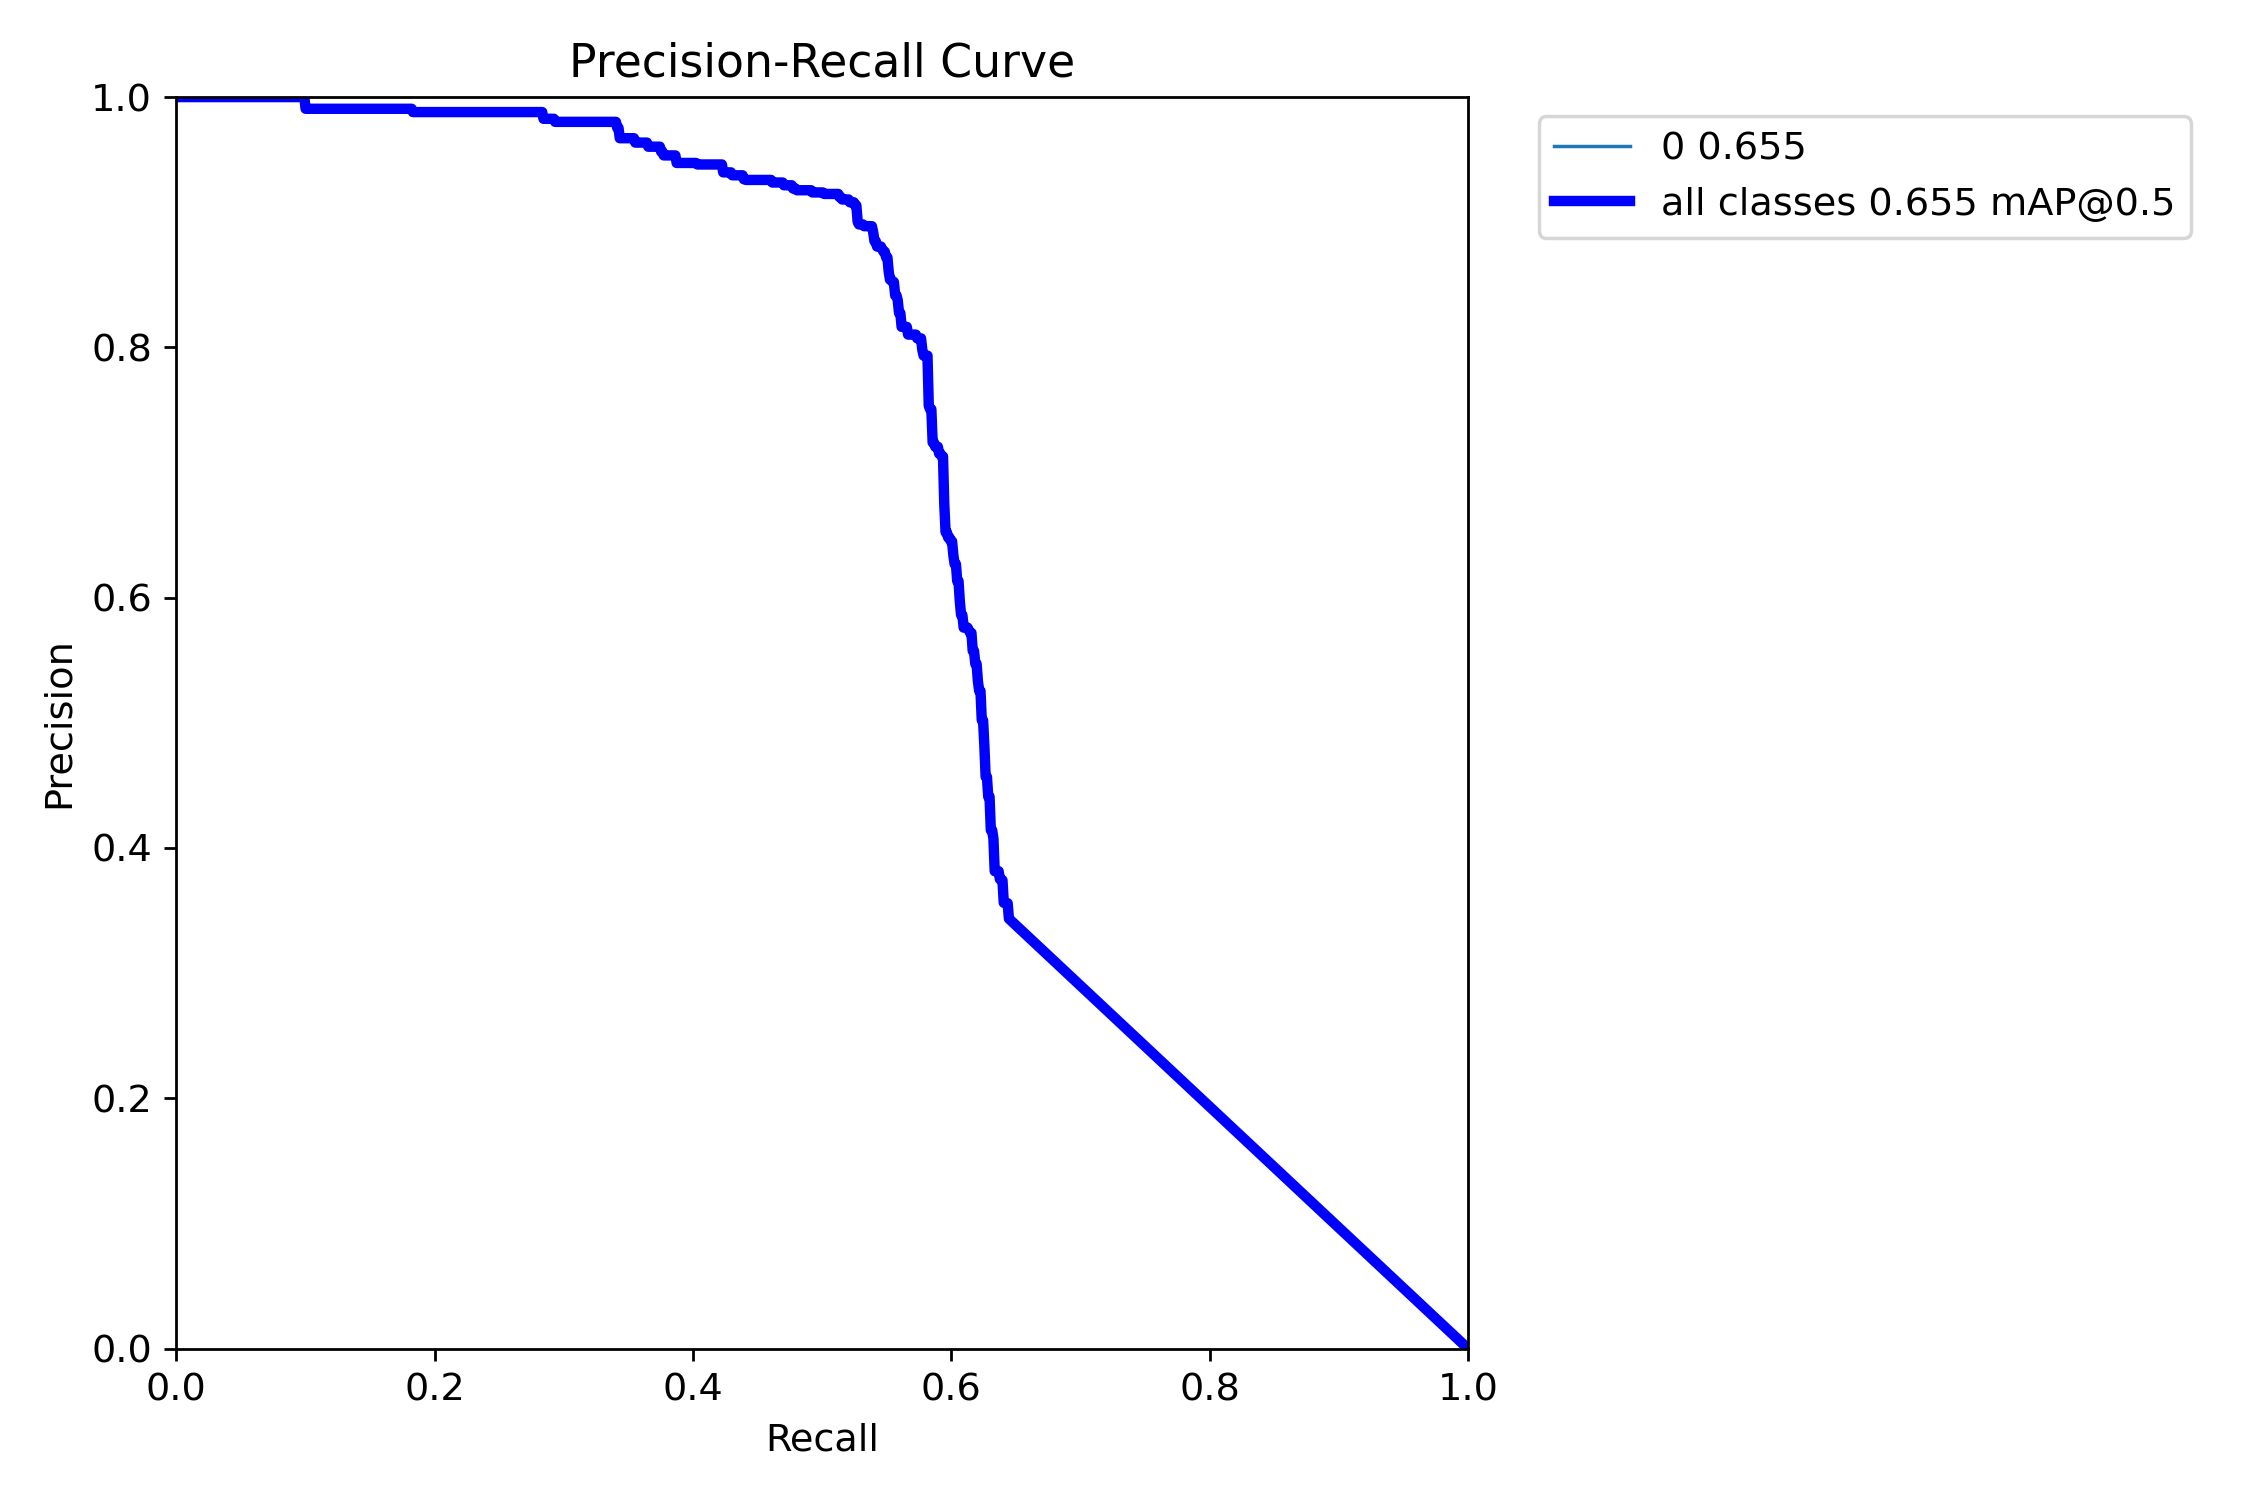
\includegraphics[width=0.9\textwidth]{./img/PR_curve-yolov11s.png}
    \caption{Curva di Precision-Recall per YOLOv11s}
    \label{fig:yolov11s-pr-curve}
\end{figure}

\begin{figure}[H]
    \centering
    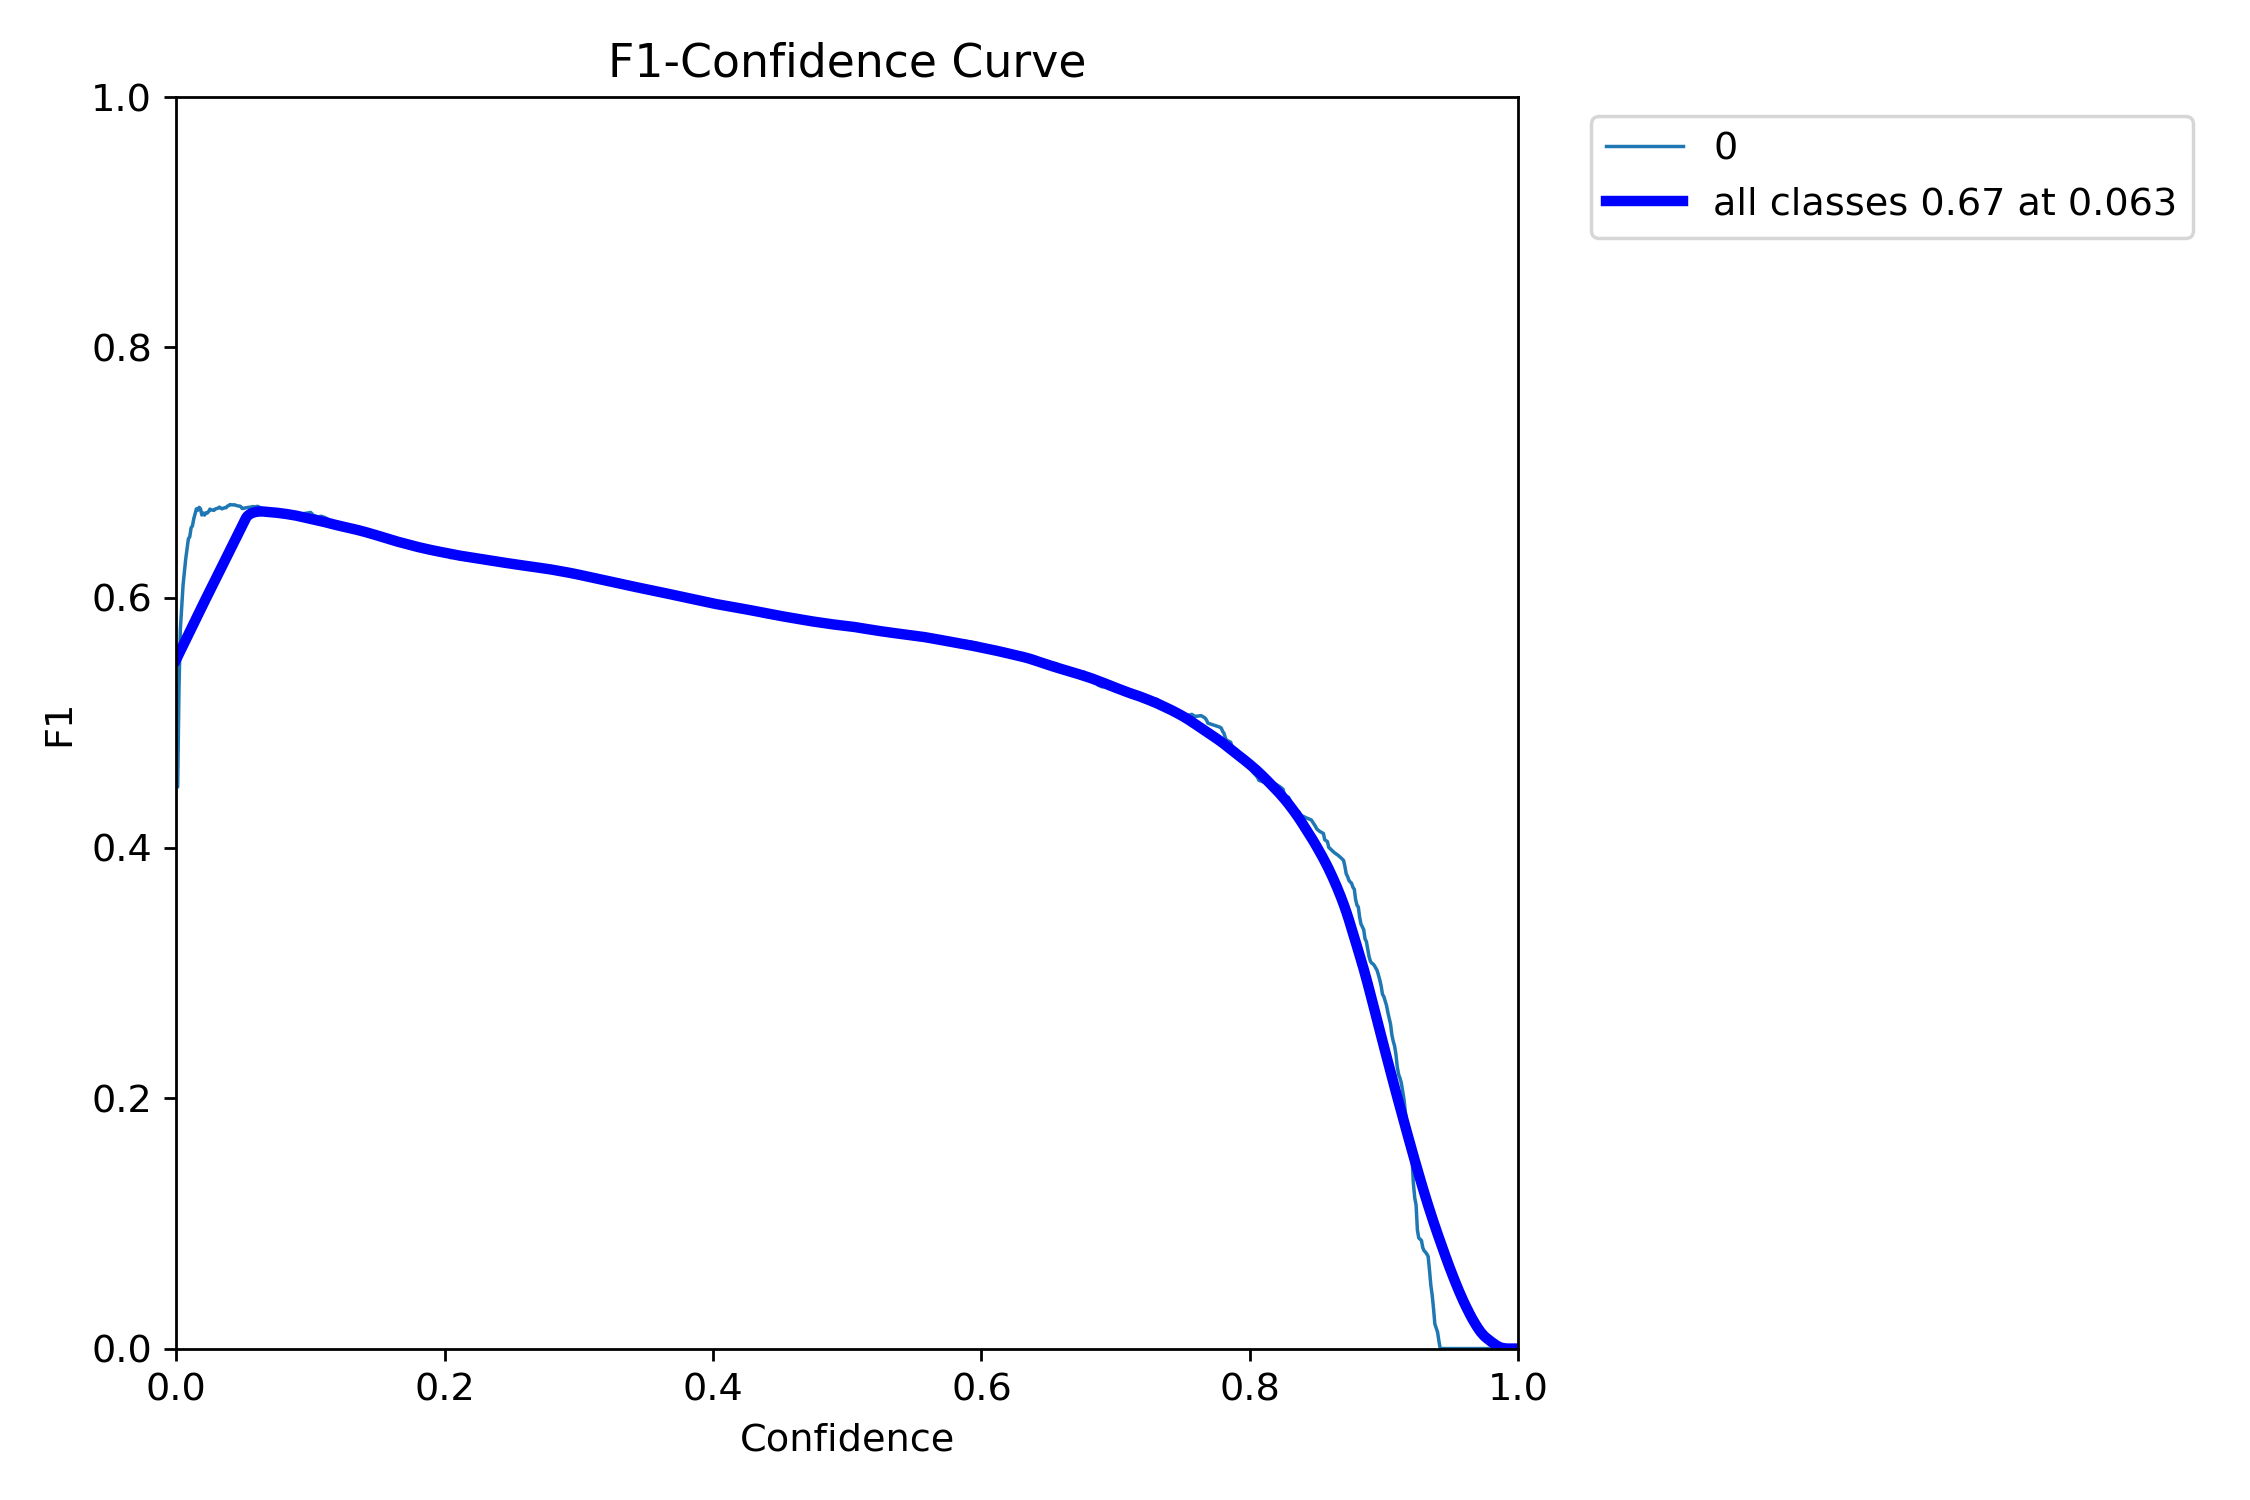
\includegraphics[width=0.9\textwidth]{./img/F1_curve-yolov11s.png}
    \caption{F1-Score per YOLOv11s}
    \label{fig:yolov11s-f1-score}
\end{figure}

\begin{figure}[H]
    \centering
    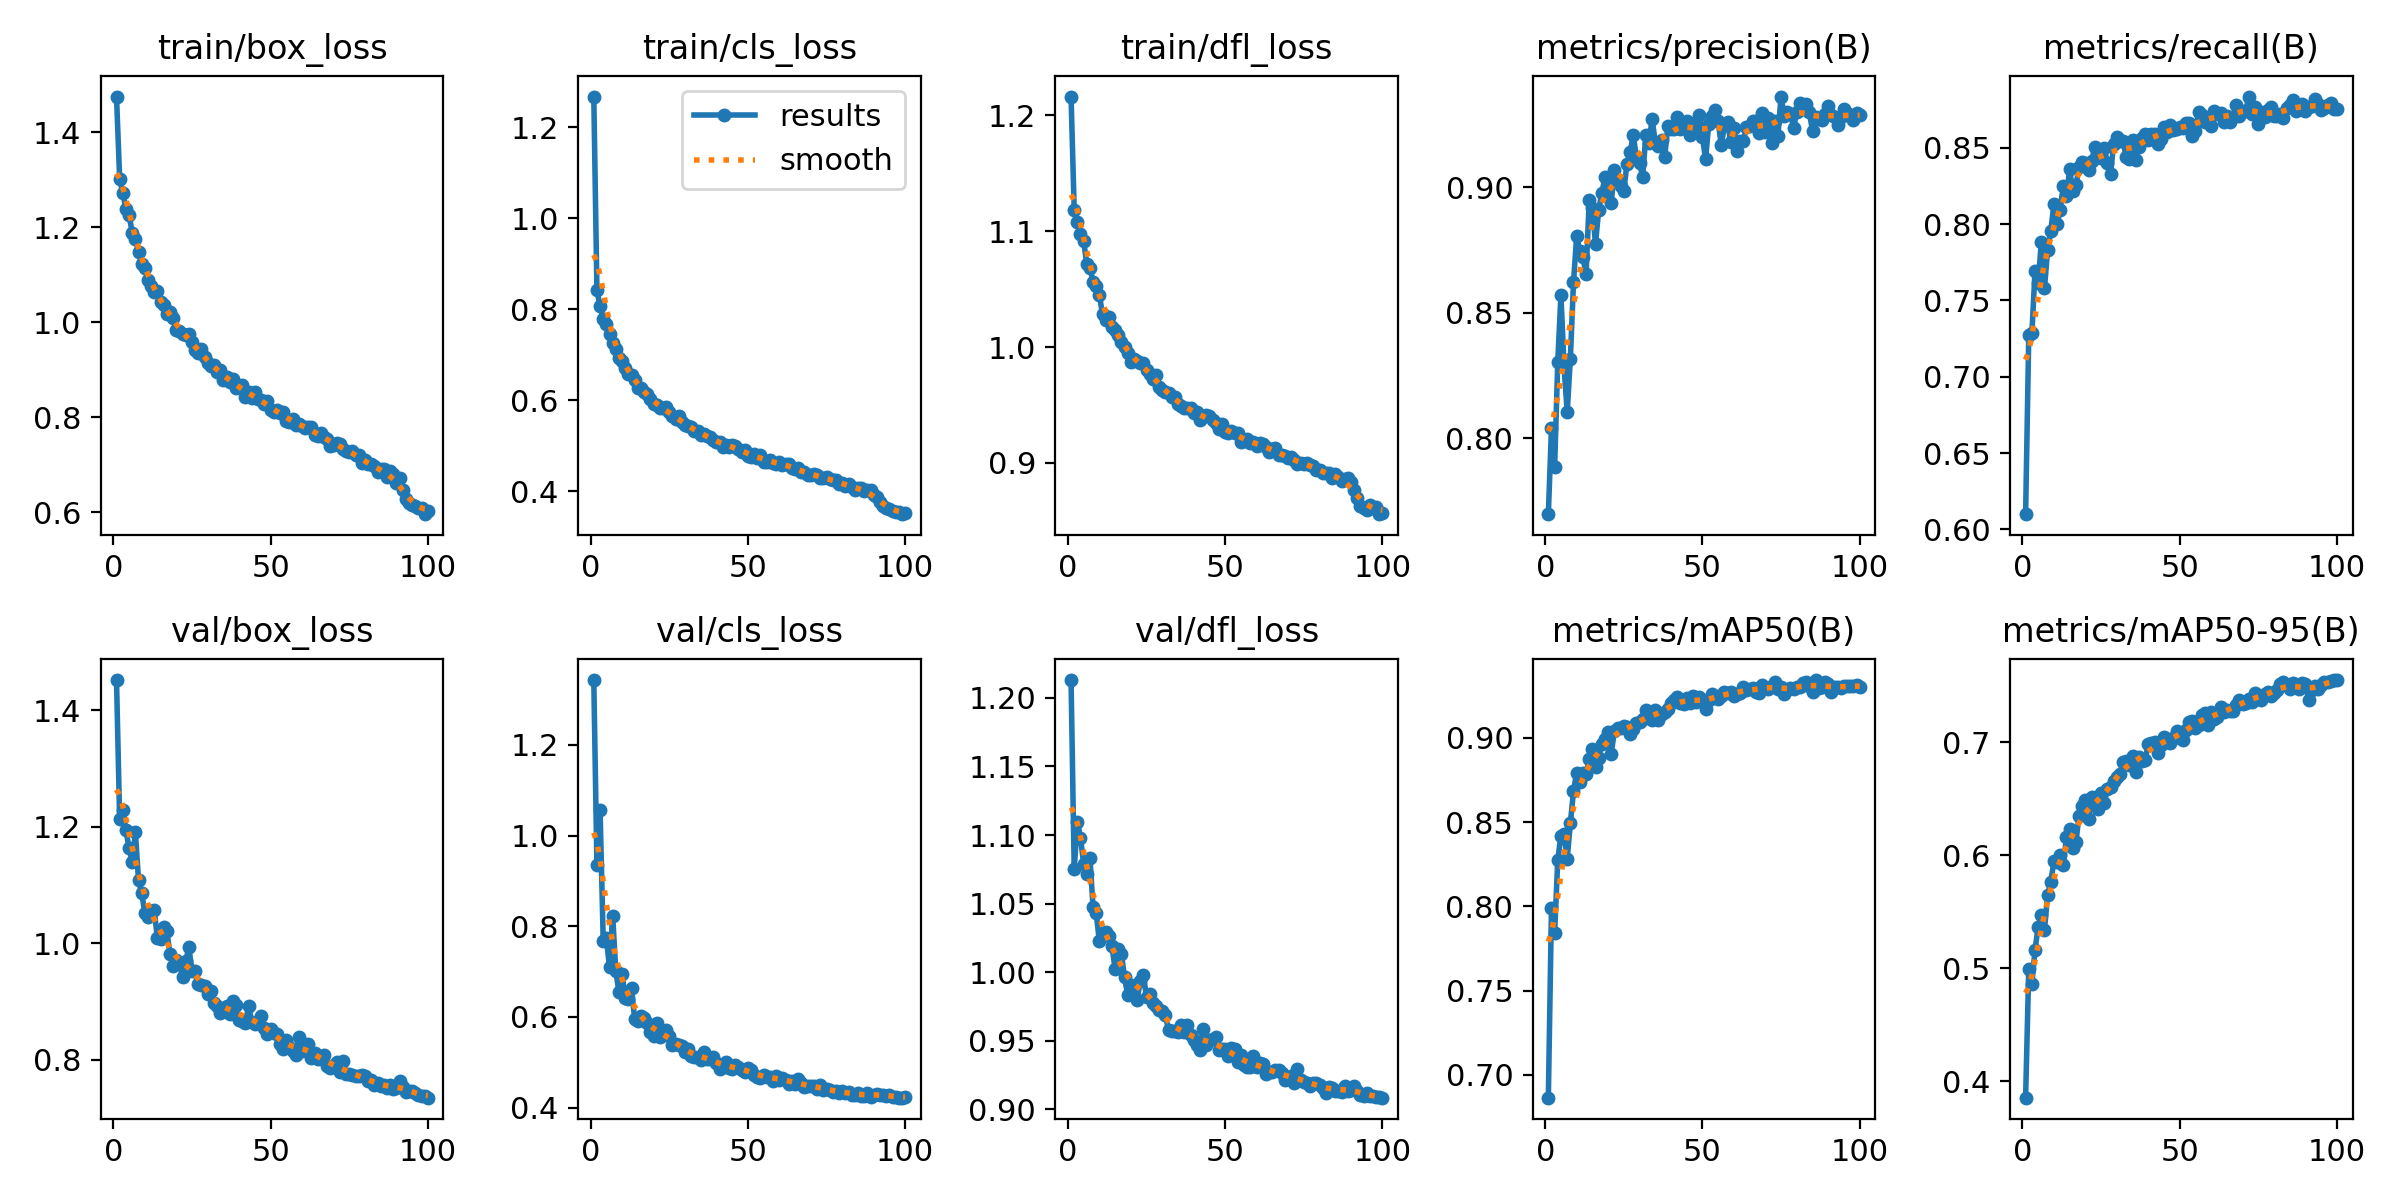
\includegraphics[width=1.1\textwidth]{./img/results-yolov11s.png}
    \caption{Risultati completi per YOLOv11s}
    \label{fig:yolov11s-results}
\end{figure}


\subsubsection{Analisi dei risultati}
Analizzando i dati presentati nelle tabelle, emerge un quadro interessante per i modelli YOLO, tutti addestrati per 100 epoche. Nel dettaglio:

\begin{itemize}
    \item \textbf{YOLOv8m} \\
    Questo modello si distingue per la sua \textbf{Precisione (0.8965)} particolarmente alta. Ciò significa che quasi il 90\% delle volte in cui rileva un oggetto e lo etichetta come "umano", la sua predizione è corretta. È un risultato notevole per evitare falsi positivi. Anche le metriche di \textbf{mAP (mAP50: 0.6555, mAP50-95: 0.3276)} sono le migliori del gruppo YOLO, indicando una buona capacità di rilevamento complessiva. Tuttavia, il suo punto debole, comune a tutti i modelli YOLO in questo contesto, è la \textbf{Recall (0.5368)}. Questo valore suggerisce che, pur essendo molto preciso nelle sue rilevazioni, riesce a identificare solo poco più della metà degli umani effettivamente presenti nel test set.

    \item \textbf{YOLOv11s} \\
    Questo modello mostra un comportamento simile al precedente, con una \textbf{Precisione (0.8035)} comunque elevata. La sua \textbf{Recall (0.5594)}, sebbene leggermente superiore a quella della versione \textit{nano}, rimane un aspetto critico. Le sue metriche di \textbf{mAP (mAP50: 0.6463, mAP50-95: 0.3333)} sono molto competitive, quasi alla pari con il modello più performante del gruppo. Questo modello rappresenta un buon equilibrio tra le versioni più piccole e quelle più grandi di YOLO, ma la sua tendenza a mancare un numero significativo di umani potrebbe essere un limite in applicazioni dove è cruciale non perdere nessuna rilevazione.

    \item \textbf{YOLOv10n} \\
    La versione \textit{nano} di YOLOv10 è progettata per essere estremamente leggera e veloce, ideale per ambienti con risorse limitate. Le sue metriche riflettono questo compromesso: pur avendo una \textbf{Precisione (0.8437)} ancora molto buona, la sua \textbf{Recall (0.4830)} è la più bassa tra i modelli YOLO testati. Questo indica non individua quasi la metà degli umani presenti nel test set. Anche le sue metriche di \textbf{mAP (mAP50: 0.5871, mAP50-95: 0.2981)} sono le più basse. È una scelta valida solo se la velocità è l'unica priorità e si può tollerare di perdere molte rilevazioni, accettando un compromesso significativo sull'accuratezza complessiva.
\end{itemize}
I modelli YOLO, pur eccellendo in precisione e mantenendo la loro intrinseca velocità, mantengono una recall medio-bassa. Sembrano essere più cauti, rilevano solo gli oggetti di cui il modello pare essere molto sicuro, ignorando quelli più difficili da individuare.

\subsection{Performance del modello Faster R-CNN (Resnet50)}
Di seguito, viene presentata una tabella riassuntiva delle performance ottenute dal modello Faster R-CNN con backbone Resnet50 sul test set acquisito.

\begin{table}[h!]
\centering
\label{tab:fasterrcnn_metrics_performance}
\begin{tabular}{|l|c|c|c|}
\hline
\textbf{Modello} & \textbf{Precisione} & \textbf{Recall} & \textbf{F1-Score} \\
\hline
Faster R-CNN (ResNet50) & 0.7956 & 0.7435 & 0.7687 \\
\hline
\end{tabular}
\caption{Risultati del modello Faster RCNN con backbone Resnet50}
\end{table}

\subsubsection{Grafici dei risultati sul train/val set}
\begin{figure}[H]
    \centering
    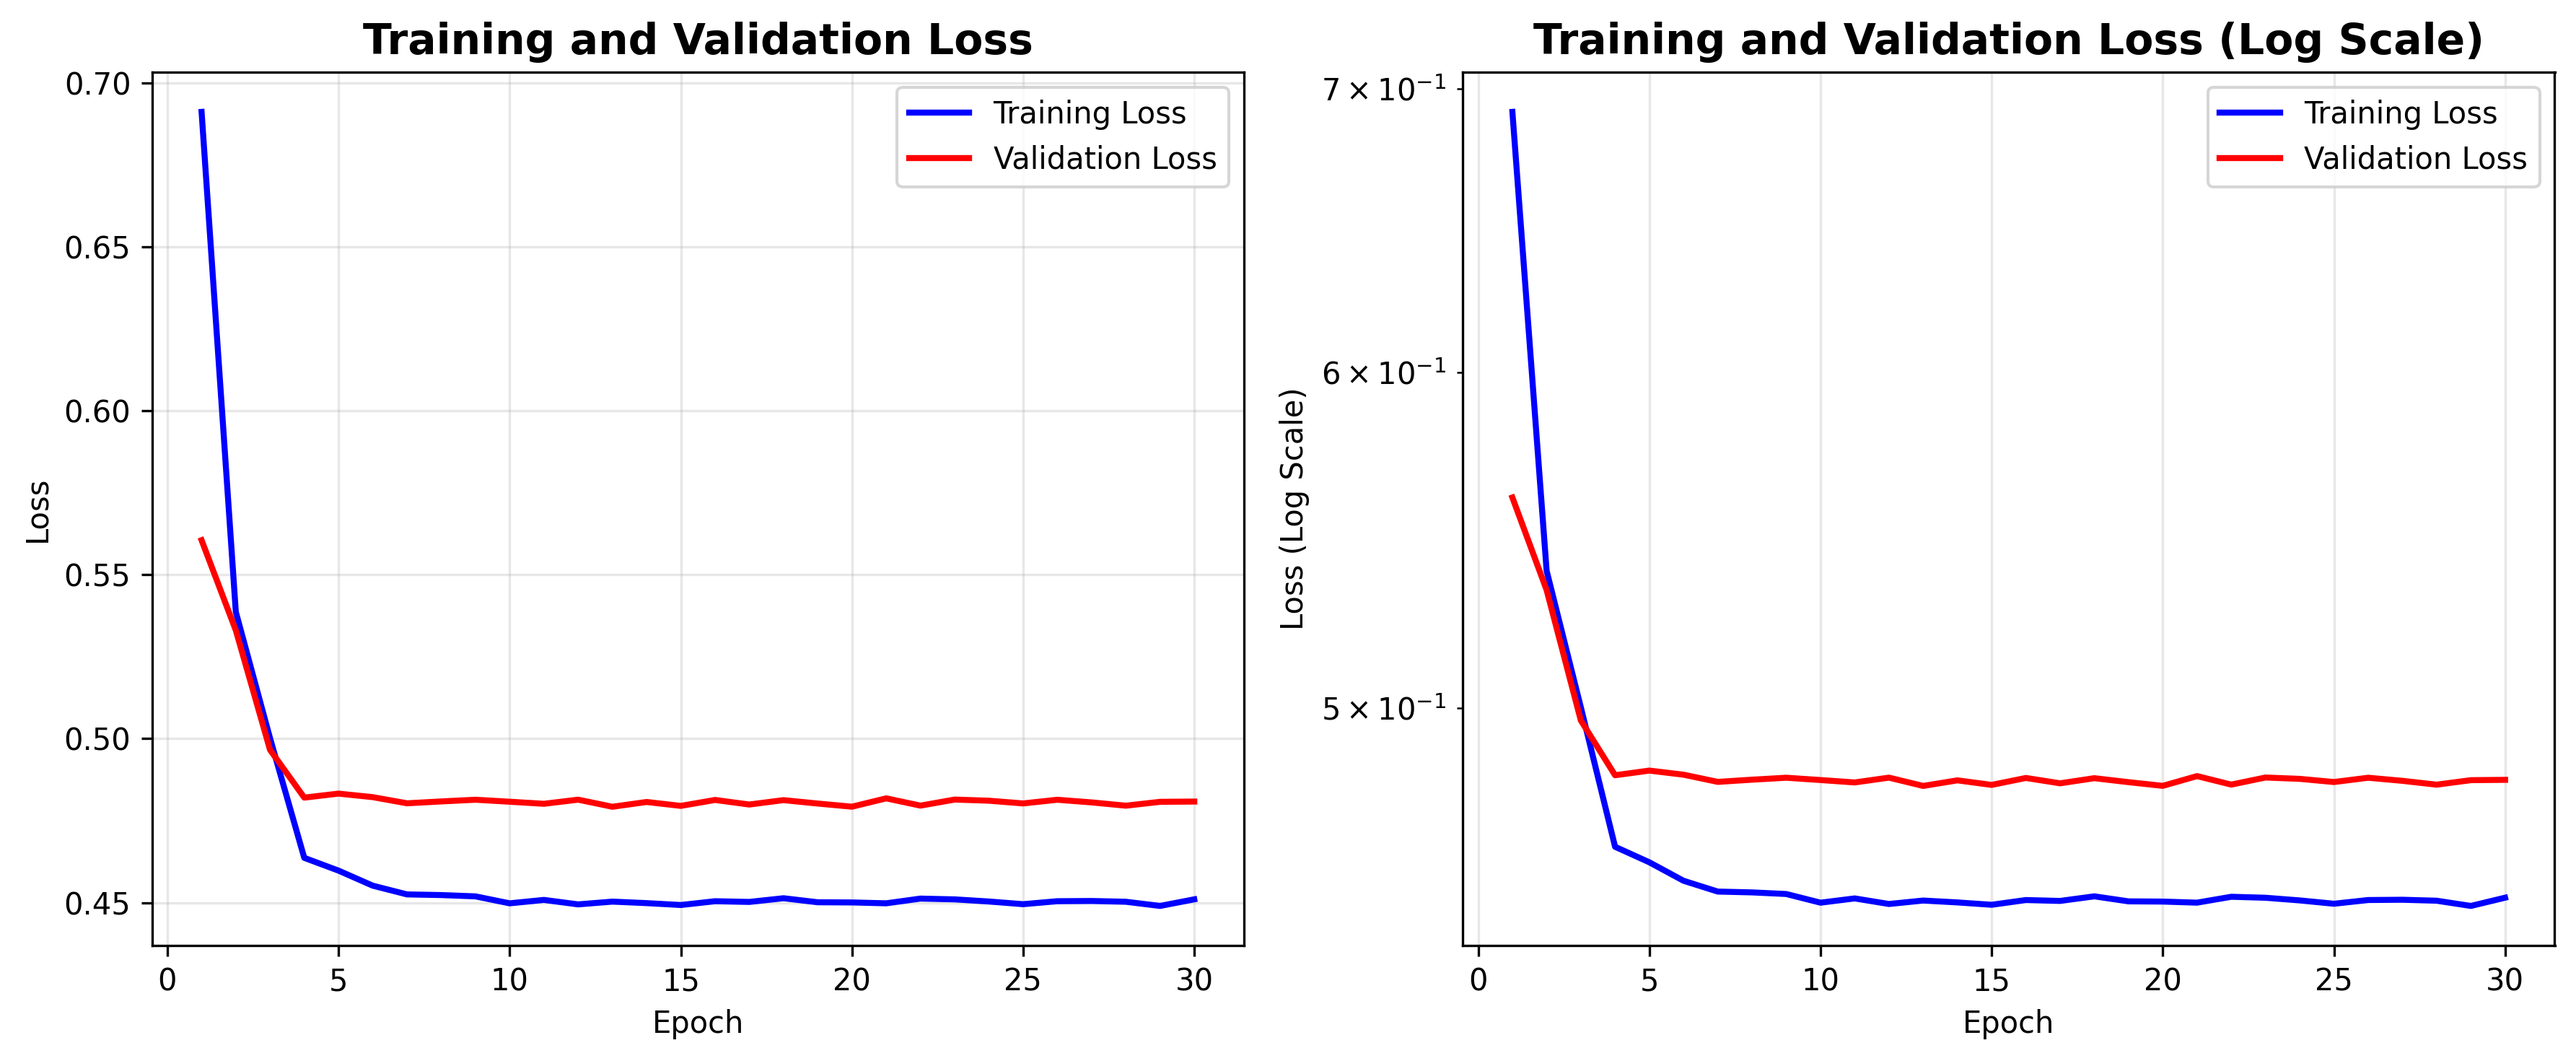
\includegraphics[width=1.00\textwidth]{./img/training_curves-resnet50.png}
    \caption{Curve di Training e Validation Loss per ResNet50}
    \label{fig:resnet50-training-curve}
\end{figure}

\subsubsection{Analisi dei risultati}
Il modello Faster R-CNN, equipaggiato con una backbone Resnet50, è stato addestrato per \textbf{30 epoche}. Pur essendo stato addestrato per un numero di epoche inferiore rispetto ai modelli YOLO, dimostra una performance notevole, soprattutto in termini di recall. \\
La sua precisione (\textbf{0.7956}) indica che quasi l'80\% delle volte in cui il modello rileva un oggetto come umano/pedone, la sua predizione è corretta. Bisogna, però, spostare l'attenzione verso la sua recall (\textbf{0.7435}). Questo valore, significativamente più alto rispetto a quello dei modelli YOLO, indica che Faster R-CNN è stato in grado di identificare circa il 74\% di tutti gli esseri umani effettivamente presenti nel test set. In applicazioni dove è cruciale non perdere nessuna rilevazione (ad esempio nella sorveglianza per la sicurezza o nella guida autonoma per la rilevazione di pedoni), una recall elevata è spesso preferibile.
L'F1-Score (0.7687), che bilancia precisione e recall, conferma l'equilibrio complessivo delle prestazioni del modello. I conteggi dettagliati ci danno un'idea più precisa: con \textbf{432 True Positives}, il modello ha rilevato correttamente un gran numero di umani. I \textbf{149 False Negatives} sono gli umani che il modello non è riuscito a rilevare. Questo quadro suggerisce che Faster R-CNN è più "aggressivo" nel trovare gli oggetti, a costo di qualche falso positivo in più, ma con il grande vantaggio di mancare meno soggetti.

\subsection{Link ai video del test set con annotazioni e ground truth}
Di seguito sarà possibile trovare i link diretti ai tre video acquisiti e utilizzati come test set. In ordine abbiamo: \textbf{IMG\_0555}, \textbf{IMG\_0559}, \textbf{IMG\_0564}. La predizione su questi video è stata fatta con YOLOv11s che ha avuto una performance migliore rispetto gli altri modelli della famiglia, e Faster R-CNN.\\
Questo è l'elenco ai video originali:
\begin{itemize}
    \item \href{https://drive.google.com/file/d/1z2SZrV0Oo12ZmZHmEnvc6FI6S2xBEjoE/view}{IMG\_0555}
    \item \href{https://drive.google.com/file/d/1FsokvyyQTtCPPU-ZIuCIpo1K5gemVwOx/view}{IMG\_0559}
    \item \href{https://drive.google.com/file/d/1L-C9DcVM4l_B8eLbezqnkduJdwJBZnd3/view}{IMG\_0564}
\end{itemize}
Qui di seguito la predizione dei risultati YOLOv11s:
\begin{itemize}
    \item \href{https://drive.google.com/file/d/1d7B1pMO5ctPi2unE_4nkdvajYZBqxDTj/view}{IMG\_0555}
    \item \href{https://drive.google.com/file/d/1D5YNEHx2KaIldo9vBqM_gRzD07-hArh5/view}{IMG\_0559}
    \item \href{https://drive.google.com/file/d/1njPmy47J4beGyqhlNW3y3yMPaNR4EntA/view}{IMG\_0564}
\end{itemize}
Ed infine i risultati di Faster R-CNN con ResNet50:
\begin{itemize}
    \item \href{https://drive.google.com/file/d/1xUAzZqYaYcdar1p-CkyW6TPmXwx6kMgs/view}{IMG\_0555}
    \item \href{https://drive.google.com/file/d/1dW8WLCrrsxh71S9F2NQbzeKWljWRUzQn/view}{IMG\_0559}
    \item \href{https://drive.google.com/file/d/1XUTXkQL84rpisBOrjzlyYpyvCGkHcwg2/view}{IMG\_0564}
\end{itemize}

\subsection{Considerazioni complessive e impatto dei fattori esterni}
I risultati ottenuti si presentano promettenti. Tuttavia, si ritiene possibile che vi siano margini di miglioramento. I risultati potrebbero essere influenzati dalla differenza di angolazione delle riprese tra il set di training e quello di test. La differenza di angolazione delle riprese tra il training set e il test set è un fattore significativo. I modelli tendono a performare meglio su dati simili a quelli su cui sono stati addestrati. Inoltre, il ridimensionamento dei video potrebbe aver introdotto un deterioramento delle caratteristiche originali e della qualità iniziale, incidendo sulle performance.


\section{Conclusione}

In conclusione, i risultati ottenuti evidenziano come tutti i modelli analizzati siano stati in grado di rilevare con successo la presenza di persone nelle immagini, sebbene con differenze significative nelle rispettive prestazioni. La famiglia \textbf{YOLO}, nelle sue versioni \textbf{v8m}, \textbf{v10n} e \textbf{v11s}, ha dimostrato un’elevata efficacia in contesti real-time, in particolare grazie ad un alto livello di \textbf{precisione} (fino a circa \textbf{0.8965} con YOLOv8m), utile a contenere il numero di falsi positivi. Tuttavia, la \textbf{recall}, generalmente inferiore (attorno al 50--55\%), suggerisce la mancata rilevazione di alcuni soggetti, soprattutto quelli meno evidenti.\\
Il modello \textbf{YOLOv8m} si è rivelato il più accurato in termini assoluti, mentre \textbf{YOLOv11s} ha offerto un buon compromesso tra accuratezza e efficienza computazionale, con un bilanciamento efficace tra precisione e recall. \textbf{YOLOv10n}, pur essendo molto efficiente dal punto di vista computazionale, ha mostrato le prestazioni più basse, specialmente nella capacità di rilevamento, risultando più adatto a scenari embedded o con risorse limitate.\\
Risulta diverso l’approccio \textit{two-stage} adottato con \textbf{Faster R-CNN} e backbone \textbf{ResNet50} il quale ha permesso di raggiungere una \textbf{recall} sensibilmente più alta (circa \textbf{0.74}), evidenziando la capacità del modello di individuare la maggior parte dei soggetti presenti nelle immagini. Il compromesso è rappresentato da una precisione leggermente inferiore, ma comunque accettabile, e da un maggior costo computazionale.\\
La scelta dei modelli dipende fortemente dal contesto applicativo:
\begin{itemize}
    \item i modelli \textbf{YOLO}, per la loro architettura single-stage, sono ideali per applicazioni real-time come sorveglianza, robotica o guida autonoma;
    \item \textbf{Faster R-CNN}, invece, è indicato in contesti in cui è fondamentale non perdere alcuna rilevazione, anche a costo di maggiori risorse computazionali.
\end{itemize}
Nel complesso, il sistema sviluppato ha confermato l'\textbf{attuabilità e l'efficacia} nell'impiego di tecnologie di Object Detection avanzate per il riconoscimento di pedoni in ambienti reali. L’utilizzo di un dataset acquisito manualmente ha permesso di testare i modelli in condizioni meno controllate rispetto ai benchmark standard, confermando la capacità dei modelli più recenti di adattarsi a contesti concreti.\vspace{1em}\\
Un ulteriore aspetto affrontato in questo lavoro è stato il \textbf{conteggio delle persone} (\textit{people counting}) nei video, funzione di rilievo in ambiti di sorveglianza e analisi del comportamento. Tale attività è stata realizzata a partire dai risultati dell'object detection, combinando le bounding box generate nei singoli frame. Sebbene la soluzione implementata non includa ancora un sistema avanzato di tracking multi-oggetto (come DeepSORT), il metodo di conteggio frame-by-frame ha fornito una prima valutazione dell'affidabilità dei modelli anche in contesto dinamico. Il risultato ha confermato che la \textbf{recall} è il parametro più critico ai fini del conteggio accurato, poiché ogni persona non rilevata comporta una sottostima sistematica.\\
Pertanto, i modelli con una recall più elevata, come \textbf{Faster R-CNN}, risultano più adatti per applicazioni dove è fondamentale evitare mancate rilevazioni, come il conteggio affidabile di flussi pedonali in ambienti reali.

\vspace{1em}
\subsection{Lezioni apprese}

Nel corso di questo progetto, sono emerse diverse considerazioni che hanno contribuito a rafforzare la comprensione pratica dei modelli di Object Detection e delle loro implicazioni nel mondo reale:

\begin{itemize}
    \item \textbf{Importanza della qualità e varietà dei dati:} la fase di raccolta manuale del dataset ha evidenziato quanto sia fondamentale disporre di immagini realistiche, differenti per angolazione, qualità e contesto ambientale. L’assenza di varietà nei dati di addestramento può compromettere significativamente la generalizzazione dei modelli, portandoli in uno stato di overfitting.

    \item \textbf{Trade-off tra accuratezza e prestazioni computazionali:} il confronto tra modelli YOLO e Faster R-CNN ha permesso di osservare direttamente come scelte architetturali diverse influenzino la velocità, la precisione e la capacità di rilevamento. In particolare, YOLO si è rivelato più adatto a contesti real-time, mentre Faster R-CNN ha eccelso nella recall, elemento cruciale per il people counting.

    \item \textbf{Criticità della recall per il conteggio:} nell’implementazione del people counting basato su Object Detection, si è notato come una bassa recall sia correlata a una sottostima del numero di persone rilevate. Ciò ha messo in luce la necessità di bilanciare meglio le metriche di valutazione in funzione dell’applicazione.

    \item \textbf{Limiti dell’assenza di tracking:} l’adozione di una soluzione frame-by-frame, priva di tracking, ha mostrato i suoi limiti nei video dinamici, in cui la stessa persona può essere conteggiata più volte o, al contrario, non rilevata in frame successivi. Questo evidenzia il ruolo fondamentale che può avere un modulo di tracking multi-oggetto (es. DeepSORT) nei sistemi di conteggio affidabili.

    \item \textbf{Apprendimento sull’intero ciclo di sviluppo:} l’esperienza maturata ha fornito una panoramica completa del workflow di un progetto di Machine Learning: dalla definizione del problema, alla raccolta e annotazione dei dati, passando per l’addestramento, la valutazione e l’impiego di tecniche di interpretazione dei risultati. Questo ha permesso di consolidare le conoscenze teoriche con un forte approccio applicativo.

\end{itemize}
In sintesi, questo progetto non solo ha permesso di mettere in pratica tecniche all'avanguardia per l’Object Detection, ma ha anche fornito una visione critica sull’importanza del contesto applicativo e delle scelte progettuali, stimolando lo sviluppo di soluzioni più complete e robuste per sfide reali di Computer Vision.

\subsection{Possibili miglioramenti}

Sulla base dell’analisi condotta, si propongono i seguenti possibili sviluppi futuri:
\begin{itemize}
    \item \textbf{Espansione del dataset e numero di epoche}: includere immagini con angolazioni, risoluzioni e scenari differenti per migliorare la generalizzazione del modello. Inoltre, sarebbe interessante aumentare il numero di epoche durante l'apprendimento per vedere come questo migliora le prestazioni. 
    
    \item \textbf{Data Augmentation mirata}: introdurre trasformazioni prospettiche, modifiche di scala e simulazioni di condizioni reali (blur, rumore, oscuramento) per rendere il training più robusto.
    
    \item \textbf{Ottimizzazione dei parametri di inferenza}: calibrare le soglie di confidenza e le strategie di NMS (dove presenti) in funzione del contesto operativo.
    
    \item \textbf{Esplorazione di architetture avanzate}: sperimentare modelli YOLO più grandi o tecniche ibride, come DETR o modelli Transformer-based.
    
    \item \textbf{Introduzione del tracking temporale}: integrare algoritmi di tracking (es. SORT o DeepSORT) per migliorare la continuità della rilevazione nei video.
    
    \item \textbf{Ottimizzazione per ambienti embedded}: valutare tecniche di quantizzazione, pruning e accelerazione hardware per un deployment efficiente su dispositivi edge.
\end{itemize}
\vspace{0.5em}
In definitiva, questo lavoro ha fornito un confronto approfondito tra approcci \textit{single-stage} e \textit{two-stage}, mettendo in evidenza vantaggi e limiti di ciascuno. I risultati ottenuti costituiscono una solida base per applicazioni reali e futuri miglioramenti, orientati verso sistemi di rilevamento sempre più \textbf{affidabili}, \textbf{veloci} e \textbf{adattabili} a diversi scenari della Computer Vision moderna.
\newpage
\begin{thebibliography}{9}

\bibitem{MOTSynth}
Matteo Fabbri et al. 
\textit{MOTSynth: How Can Synthetic Data Help Pedestrian Detection and Tracking?
},
ICCV 2021.

\bibitem{Roboflow}
Denise Cilia, Eleonora Giuffrida, Valeria Platania:
\textit{New Dataset For Machine Learning Project},
\href{https://app.roboflow.com/test-hqhgt/new-dataset-for-ml-project/5}{Link}

\bibitem{ResNet50}
He, K., Zhang, X., Ren, S., Sun, J. (2016)
\textit{Deep Residual Learning for Image Recognition},
In Proceedings of the IEEE Conference on Computer Vision and Pattern Recognition (CVPR)

\bibitem{FasterRCNN}
Ren, S., He, K., Girshick, R., Sun, J. (2015)
\textit{Faster R-CNN: Towards Real-Time Object Detection with Region Proposal Networks}
NIPS'15: Proceedings of the 29th International Conference on Neural Information Processing Systems - Volume 1

\bibitem{YOLOv11}
Khanam, R. Hussain, M. (2024) 
\textit{YOLOv11: An Overview of the Key Architectural Enhancements.}

\bibitem{YOLO}
Redmon, J. et al. (2016)
\textit{You Only Look Once: Unified, Real-Time Object Detection.}

\end{thebibliography}

\end{document}


